
%% bare_conf.tex
%% V1.4a
%% 2014/09/17
%% by Michael Shell
%% See:
%% http://www.michaelshell.org/
%% for current contact information.
%%
%% This is a skeleton file demonstrating the use of IEEEtran.cls
%% (requires IEEEtran.cls version 1.8a or later) with an IEEE
%% conference paper.
%%
%% Support sites:
%% http://www.michaelshell.org/tex/ieeetran/
%% http://www.ctan.org/tex-archive/macros/latex/contrib/IEEEtran/
%% and
%% http://www.ieee.org/

%%*************************************************************************
%% Legal Notice:
%% This code is offered as-is without any warranty either expressed or
%% implied; without even the implied warranty of MERCHANTABILITY or
%% FITNESS FOR A PARTICULAR PURPOSE! 
%% User assumes all risk.
%% In no event shall IEEE or any contributor to this code be liable for
%% any damages or losses, including, but not limited to, incidental,
%% consequential, or any other damages, resulting from the use or misuse
%% of any information contained here.
%%
%% All comments are the opinions of their respective authors and are not
%% necessarily endorsed by the IEEE.
%%
%% This work is distributed under the LaTeX Project Public License (LPPL)
%% ( http://www.latex-project.org/ ) version 1.3, and may be freely used,
%% distributed and modified. A copy of the LPPL, version 1.3, is included
%% in the base LaTeX documentation of all distributions of LaTeX released
%% 2003/12/01 or later.
%% Retain all contribution notices and credits.
%% ** Modified files should be clearly indicated as such, including  **
%% ** renaming them and changing author support contact information. **
%%
%% File list of work: IEEEtran.cls, IEEEtran_HOWTO.pdf, bare_adv.tex,
%%                    bare_conf.tex, bare_jrnl.tex, bare_conf_compsoc.tex,
%%                    bare_jrnl_compsoc.tex, bare_jrnl_transmag.tex
%%*************************************************************************


% *** Authors should verify (and, if needed, correct) their LaTeX system  ***
% *** with the testflow diagnostic prior to trusting their LaTeX platform ***
% *** with production work. IEEE's font choices and paper sizes can       ***
% *** trigger bugs that do not appear when using other class files.       ***                          ***
% The testflow support page is at:
% http://www.michaelshell.org/tex/testflow/



\documentclass[conference]{IEEEtran}
%\documentclass[10pt]{IEEEtran}
% Some Computer Society conferences also require the compsoc mode option,
% but others use the standard conference format.
%
% If IEEEtran.cls has not been installed into the LaTeX system files,
% manually specify the path to it like:
% \documentclass[conference]{../sty/IEEEtran}

% Some very useful LaTeX packages include:
% (uncomment the ones you want to load)


% *** MISC UTILITY PACKAGES ***
%
%\usepackage{ifpdf}
% Heiko Oberdiek's ifpdf.sty is very useful if you need conditional
% compilation based on whether the output is pdf or dvi.
% usage:
% \ifpdf
%   % pdf code
% \else
%   % dvi code
% \fi
% The latest version of ifpdf.sty can be obtained from:
% http://www.ctan.org/tex-archive/macros/latex/contrib/oberdiek/
% Also, note that IEEEtran.cls V1.7 and later provides a builtin
% \ifCLASSINFOpdf conditional that works the same way.
% When switching from latex to pdflatex and vice-versa, the compiler may
% have to be run twice to clear warning/error messages.

% *** CITATION PACKAGES ***
%
%\usepackage{cite}
% cite.sty was written by Donald Arseneau
% V1.6 and later of IEEEtran pre-defines the format of the cite.sty package
% \cite{} output to follow that of IEEE. Loading the cite package will
% result in citation numbers being automatically sorted and properly
% "compressed/ranged". e.g., [1], [9], [2], [7], [5], [6] without using
% cite.sty will become [1], [2], [5]--[7], [9] using cite.sty. cite.sty's
% \cite will automatically add leading space, if needed. Use cite.sty's
% noadjust option (cite.sty V3.8 and later) if you want to turn this off
% such as if a citation ever needs to be enclosed in parenthesis.
% cite.sty is already installed on most LaTeX systems. Be sure and use
% version 5.0 (2009-03-20) and later if using hyperref.sty.
% The latest version can be obtained at:
% http://www.ctan.org/tex-archive/macros/latex/contrib/cite/
% The documentation is contained in the cite.sty file itself.

% *** GRAPHICS RELATED PACKAGES ***
%
\ifCLASSINFOpdf
  % \usepackage[pdftex]{graphicx}
  % declare the path(s) where your graphic files are
  % \graphicspath{{../pdf/}{../jpeg/}}
  % and their extensions so you won't have to specify these with
  % every instance of \includegraphics
  % \DeclareGraphicsExtensions{.pdf,.jpeg,.png}
\else
  % or other class option (dvipsone, dvipdf, if not using dvips). graphicx
  % will default to the driver specified in the system graphics.cfg if no
  % driver is specified.
  % \usepackage[dvips]{graphicx}
  % declare the path(s) where your graphic files are
  % \graphicspath{{../eps/}}
  % and their extensions so you won't have to specify these with
  % every instance of \includegraphics
  % \DeclareGraphicsExtensions{.eps}
\fi
% graphicx was written by David Carlisle and Sebastian Rahtz. It is
% required if you want graphics, photos, etc. graphicx.sty is already
% installed on most LaTeX systems. The latest version and documentation
% can be obtained at: 
% http://www.ctan.org/tex-archive/macros/latex/required/graphics/
% Another good source of documentation is "Using Imported Graphics in
% LaTeX2e" by Keith Reckdahl which can be found at:
% http://www.ctan.org/tex-archive/info/epslatex/
%
% latex, and pdflatex in dvi mode, support graphics in encapsulated
% postscript (.eps) format. pdflatex in pdf mode supports graphics
% in .pdf, .jpeg, .png and .mps (metapost) formats. Users should ensure
% that all non-photo figures use a vector format (.eps, .pdf, .mps) and
% not a bitmapped formats (.jpeg, .png). IEEE frowns on bitmapped formats
% which can result in "jaggedy"/blurry rendering of lines and letters as
% well as large increases in file sizes.
%
% You can find documentation about the pdfTeX application at:
% http://www.tug.org/applications/pdftex





% *** MATH PACKAGES ***
%
%\usepackage[cmex10]{amsmath}
% A popular package from the American Mathematical Society that provides
% many useful and powerful commands for dealing with mathematics. If using
% it, be sure to load this package with the cmex10 option to ensure that
% only type 1 fonts will utilized at all point sizes. Without this option,
% it is possible that some math symbols, particularly those within
% footnotes, will be rendered in bitmap form which will result in a
% document that can not be IEEE Xplore compliant!
%
% Also, note that the amsmath package sets \interdisplaylinepenalty to 10000
% thus preventing page breaks from occurring within multiline equations. Use:
%\interdisplaylinepenalty=2500
% after loading amsmath to restore such page breaks as IEEEtran.cls normally
% does. amsmath.sty is already installed on most LaTeX systems. The latest
% version and documentation can be obtained at:
% http://www.ctan.org/tex-archive/macros/latex/required/amslatex/math/





% *** SPECIALIZED LIST PACKAGES ***
%
%\usepackage{algorithmic}
% algorithmic.sty was written by Peter Williams and Rogerio Brito.
% This package provides an algorithmic environment fo describing algorithms.
% You can use the algorithmic environment in-text or within a figure
% environment to provide for a floating algorithm. Do NOT use the algorithm
% floating environment provided by algorithm.sty (by the same authors) or
% algorithm2e.sty (by Christophe Fiorio) as IEEE does not use dedicated
% algorithm float types and packages that provide these will not provide
% correct IEEE style captions. The latest version and documentation of
% algorithmic.sty can be obtained at:
% http://www.ctan.org/tex-archive/macros/latex/contrib/algorithms/
% There is also a support site at:
% http://algorithms.berlios.de/index.html
% Also of interest may be the (relatively newer and more customizable)
% algorithmicx.sty package by Szasz Janos:
% http://www.ctan.org/tex-archive/macros/latex/contrib/algorithmicx/




% *** ALIGNMENT PACKAGES ***
%
%\usepackage{array}
% Frank Mittelbach's and David Carlisle's array.sty patches and improves
% the standard LaTeX2e array and tabular environments to provide better
% appearance and additional user controls. As the default LaTeX2e table
% generation code is lacking to the point of almost being broken with
% respect to the quality of the end results, all users are strongly
% advised to use an enhanced (at the very least that provided by array.sty)
% set of table tools. array.sty is already installed on most systems. The
% latest version and documentation can be obtained at:
% http://www.ctan.org/tex-archive/macros/latex/required/tools/


% IEEEtran contains the IEEEeqnarray family of commands that can be used to
% generate multiline equations as well as matrices, tables, etc., of high
% quality.




% *** SUBFIGURE PACKAGES ***
%\ifCLASSOPTIONcompsoc
%  \usepackage[caption=false,font=normalsize,labelfont=sf,textfont=sf]{subfig}
%\else
%  \usepackage[caption=false,font=footnotesize]{subfig}
%\fi
% subfig.sty, written by Steven Douglas Cochran, is the modern replacement
% for subfigure.sty, the latter of which is no longer maintained and is
% incompatible with some LaTeX packages including fixltx2e. However,
% subfig.sty requires and automatically loads Axel Sommerfeldt's caption.sty
% which will override IEEEtran.cls' handling of captions and this will result
% in non-IEEE style figure/table captions. To prevent this problem, be sure
% and invoke subfig.sty's "caption=false" package option (available since
% subfig.sty version 1.3, 2005/06/28) as this is will preserve IEEEtran.cls
% handling of captions.
% Note that the Computer Society format requires a larger sans serif font
% than the serif footnote size font used in traditional IEEE formatting
% and thus the need to invoke different subfig.sty package options depending
% on whether compsoc mode has been enabled.
%
% The latest version and documentation of subfig.sty can be obtained at:
% http://www.ctan.org/tex-archive/macros/latex/contrib/subfig/




% *** FLOAT PACKAGES ***
%
%\usepackage{fixltx2e}
% fixltx2e, the successor to the earlier fix2col.sty, was written by
% Frank Mittelbach and David Carlisle. This package corrects a few problems
% in the LaTeX2e kernel, the most notable of which is that in current
% LaTeX2e releases, the ordering of single and double column floats is not
% guaranteed to be preserved. Thus, an unpatched LaTeX2e can allow a
% single column figure to be placed prior to an earlier double column
% figure. The latest version and documentation can be found at:
% http://www.ctan.org/tex-archive/macros/latex/base/


%\usepackage{stfloats}
% stfloats.sty was written by Sigitas Tolusis. This package gives LaTeX2e
% the ability to do double column floats at the bottom of the page as well
% as the top. (e.g., "\begin{figure*}[!b]" is not normally possible in
% LaTeX2e). It also provides a command:
%\fnbelowfloat
% to enable the placement of footnotes below bottom floats (the standard
% LaTeX2e kernel puts them above bottom floats). This is an invasive package
% which rewrites many portions of the LaTeX2e float routines. It may not work
% with other packages that modify the LaTeX2e float routines. The latest
% version and documentation can be obtained at:
% http://www.ctan.org/tex-archive/macros/latex/contrib/sttools/
% Do not use the stfloats baselinefloat ability as IEEE does not allow
% \baselineskip to stretch. Authors submitting work to the IEEE should note
% that IEEE rarely uses double column equations and that authors should try
% to avoid such use. Do not be tempted to use the cuted.sty or midfloat.sty
% packages (also by Sigitas Tolusis) as IEEE does not format its papers in
% such ways.
% Do not attempt to use stfloats with fixltx2e as they are incompatible.
% Instead, use Morten Hogholm'a dblfloatfix which combines the features
% of both fixltx2e and stfloats:
%
% \usepackage{dblfloatfix}
% The latest version can be found at:
% http://www.ctan.org/tex-archive/macros/latex/contrib/dblfloatfix/




% *** PDF, URL AND HYPERLINK PACKAGES ***
%
%\usepackage{url}
% url.sty was written by Donald Arseneau. It provides better support for
% handling and breaking URLs. url.sty is already installed on most LaTeX
% systems. The latest version and documentation can be obtained at:
% http://www.ctan.org/tex-archive/macros/latex/contrib/url/
% Basically, \url{my_url_here}.




% *** Do not adjust lengths that control margins, column widths, etc. ***
% *** Do not use packages that alter fonts (such as pslatex).         ***
% There should be no need to do such things with IEEEtran.cls V1.6 and later.
% (Unless specifically asked to do so by the journal or conference you plan
% to submit to, of course. )

\usepackage[dvipsnames]{xcolor}
\usepackage{amsmath}
\usepackage{amssymb}
\usepackage{xspace}
\usepackage{graphicx}
\usepackage{latexsym}
\usepackage{listings}
\usepackage{multirow}
\usepackage{suffix}
\usepackage{url}
\usepackage{mathptmx}
\usepackage{mathrsfs}
\usepackage{comment}
\usepackage{enumerate}
\usepackage{txfonts}
\usepackage{hyperref}
\usepackage{fancybox}
\usepackage{space}
\usepackage{color}      % use if color is used in text

% correct bad hyphenation here
\hyphenation{op-tical net-works semi-conduc-tor}

\begin{document}
%
% paper title
% Titles are generally capitalized except for words such as a, an, and, as,
% at, but, by, for, in, nor, of, on, or, the, to and up, which are usually
% not capitalized unless they are the first or last word of the title.
% Linebreaks \\ can be used within to get better formatting as desired.
% Do not put math or special symbols in the title.
\title{\LARGE Core Higher-Order Session Processes:\\ Tractable Equivalences and Relative Expressiveness}

% author names and affiliations
% use a multiple column layout for up to three different
% affiliations
\author{
\IEEEauthorblockN{
Dimitrios Kouzapas
}
\IEEEauthorblockA{
Imperial College London	
}
\and
\IEEEauthorblockN{
Jorge A. P\'{e}rez
}
\IEEEauthorblockA{
University of Groningen
}
\and 
\IEEEauthorblockN{
Nobuko Yoshida
}
\IEEEauthorblockA{
Imperial College London	
}
}

\maketitle

%%%%%%%%%%%%%%%%%%%%%%%%%%%%%%%%%%%%%%%%%%%%%%%%%%%%%%%%%%%%%%%%%%%%%%%%%%%%%%%%%%%%%%%%%%%%%%%%%%%%
% Contents
% --------

% 1.  Formating
% 2.  Maths - Theorems
% 3.  The pi Calculus
% 4.  Session Syntax
% 5.  Subject Reduction
% 6.  Global Session Types
% 7.  Global Session Types Equivalence
% 8.  Projection
% 9.  Local Session Types
% 10. Behavioural Theory
% 11. Typed Transitions - Reductions
% 12. Typed Relations
% 13. Confluence Determinacy
% 14. Mapping
% 15. pi Constructs
% 16. LN Transform
% 17. General Types Processes Names Sessions ETC
% 18. newtheorem - newenvironment
% 19. Misc
%%%%%%%%%%%%%%%%%%%%%%%%%%%%%%%%%%%%%%%%%%%%%%%%%%%%%%%%%%%%%%%%%%%%%%%%%%%%%%%%%%%%%%%%%%%%%%%%%%%%


%%%%%%%%%%%%%%%%%%%%%%%%%%%%%%%%%%%%%%%%%%%%%%%%%%%%%%%%%%%%%%%%%%%%%%%%%%%%%%%%%%%%%%%%%%%%%%%%%%%%
%                                       FORMATING
%%%%%%%%%%%%%%%%%%%%%%%%%%%%%%%%%%%%%%%%%%%%%%%%%%%%%%%%%%%%%%%%%%%%%%%%%%%%%%%%%%%%%%%%%%%%%%%%%%%%

% Symbols
\newcommand{\semicolon}{:}
%\newcommand{\colon}{;}
\newcommand{\lrangle}[1]{\langle #1 \rangle}
\newcommand{\blrangle}[1]{\big\langle #1 \big\rangle}

%Tags
\newcommand{\parenthtext}[1]{(\textrm{\small #1})}
\newcommand{\brtext}[1]{[\textrm{\small #1}]}
\newcommand{\textinmath}[1]{\textrm{#1}}
\newcommand{\srule}[1]{\parenthtext{#1}}
\newcommand{\strule}[1]{\textrm{#1}}
\newcommand{\stypes}[1]{{\footnotesize \parenthtext{#1}}}
\newcommand{\ltsrule}[1]{{\footnotesize \lrangle{\textrm{#1}}}}
\newcommand{\eltsrule}[1]{{\footnotesize [\textrm{#1}]}}
\newcommand{\trule}[1]{{\footnotesize\brtext{#1}}}
\newcommand{\orule}[1]{{\scriptsize{\brtext{#1}}}}
\newcommand{\mrule}[1]{{\footnotesize{\parenthtext{#1}}}}

\newcommand{\iftag}{{\textrm{if }}}

% General
\newcommand{\noi}{\noindent}
\newcommand{\Hline}{\rule{\linewidth}{.5pt}}
\newcommand{\Hlinefig}{\rule{\linewidth}{.5pt}\vspace{-4mm}}
\newcommand{\myparagraph}[1]{\noindent{\textbf{#1}\ }}
\newcommand{\jparagraph}[1]{\paragraph{\textbf{#1}}}

%%%%%%%%%%%%%%%%%%%%%%%%%%%%%%%%%%%%%%%%%%%%%%%%%%%%%%%%%%%%%%%%%%%%%%%%%%%%%%%%%%%%%%%%%%%%%%%%%%%%
%                                       MATHS - THEOREMS
%%%%%%%%%%%%%%%%%%%%%%%%%%%%%%%%%%%%%%%%%%%%%%%%%%%%%%%%%%%%%%%%%%%%%%%%%%%%%%%%%%%%%%%%%%%%%%%%%%%%

%\newtheorem{notation}[definition]{Notation}

% BNF form
\newcommand{\bnfis}{\;\;::=\;\;}
\newcommand{\bnfbar}{\;\;\;|\;\;\;}
\newcommand{\sbnfbar}{\;\;|\;\;}

% Proof
\newcommand{\Case}[1]{\noi {\bf Case: }#1\\}
\newcommand{\proofend}{\qed}
%\newcommand{\proofend}{}
\newcommand{\Proof}{\noi {\bf Proof: }}

% Logic
\newcommand{\LogAnd}{\texttt{ and }}
\newcommand{\LogOr}{\texttt{ or }}

% Induction

\newcommand{\basic}{\noi {\bf Basic Step:}\\}
\newcommand{\inductive}{\noi {\bf Inductive Hypothesis:}\\}
\newcommand{\induction}{\noi {\bf Induction Step:}\\}

% Tree

\newcommand{\tree}[2]{
\ensuremath{\displaystyle
		\frac
		{
			%%\raisebox{0.0mm}{$\displaystyle{#1}$}
			#1
			%\vspace{0mm}
		}{
			%\vspace{2mm}
			#2
			%\raisebox{-0.4mm}{$\displaystyle{#2}$}
		}
	}
}


%\newcommand{\tree}[2]{
%\begin{prooftree}
%	#1
%	\justifies
%	#2
%\end{prooftree}
%}

\newcommand{\treeusing}[3]{
\begin{prooftree}
	#1
	\justifies
	#2
	\using
	#3
\end{prooftree}}

% Vectors
\newcommand{\vect}[1]{\tilde{#1}}
\newcommand{\mytilde}[1]{\widetilde{#1}}

% Functions - Set theory
\newcommand{\set}[1]{\{#1\}}
\newcommand{\es}{\emptyset}
\newcommand{\maxset}[1]{\max(#1)}
\newcommand{\setbar}{\ \ |\ \ }
\newcommand{\tuple}[2]{(#1, #2)}
\newcommand{\suchthat}{\cdot}
\newcommand{\powerset}[1]{\mathcal{P}(#1)}
\newcommand{\product}{\times}

\newcommand{\eval}{\downarrow}

\newcommand{\setsubtr}[2]{#1 \backslash #2}

\newcommand{\func}[2]{#1(#2)}
\newcommand{\dom}[1]{\mathtt{dom}(#1)}
\newcommand{\codom}[1]{\mathtt{codom}(#1)}

\newcommand{\funcbr}[2]{#1\lrangle{#2}}

\newcommand{\entails}{\text{implies}}


%%%%%%%%%%%%%%%%%%%%%%%%%%%%%%%%%%%%%%%%%%%%%%%%%%%%%%%%%%%%%%%%%%%%%%%%%%%%%%%%%%%%%%%%%%%%%%%%%%%%
%                                        pi - CALCULUS
%%%%%%%%%%%%%%%%%%%%%%%%%%%%%%%%%%%%%%%%%%%%%%%%%%%%%%%%%%%%%%%%%%%%%%%%%%%%%%%%%%%%%%%%%%%%%%%%%%%%

% Free-Bound notation
\newcommand{\freev}[1]{\lrangle{#1}}
\newcommand{\boundv}[1]{(#1)}

% General pi calculus Syntax
\newcommand{\send}[1]{\overline{#1}}
\newcommand{\ol}[1]{\overline{#1}}
\newcommand{\receive}[1]{#1.}
\newcommand{\inact}{\mathbf{0}}
\newcommand{\If}{\sessionfont{if}\ }
\newcommand{\Then}{\sessionfont{then}\ }
\newcommand{\Else}{\sessionfont{else}\ }
\newcommand{\ifthen}[2]{\If #1\ \Then #2\ }
\newcommand{\ifthenelse}[3]{\ifthen{#1}{#2} \Else #3}
\newcommand{\Par}{\;|\;}
\newcommand{\news}[1]{(\nu\, #1)}
\newcommand{\newsp}[2]{(\nu\, #1)(#2)}
\newcommand{\varp}[1]{#1}
%\newcommand{\rvar}[1]{\mathcal{#1}}
\newcommand{\rvar}[1]{#1}
%\newcommand{\rec}[2]{\mu #1. #2}
\newcommand{\recp}[2]{\mu \rvar{#1}. #2}

\newcommand{\Def}{\sessionfont{def}\ }

\newcommand{\defeq}{\stackrel{\Def}{=}}

\newcommand{\repl}{\ast\,}
\newcommand{\parcomp}[2]{\prod_{#1}{#2}}

% Free-Bound-Names sets
\newcommand{\bn}[1]{\mathtt{bn}(#1)}
\newcommand{\fn}[1]{\mathtt{fn}(#1)}
\newcommand{\ofn}[1]{\mathsf{ofn}(#1)}
\newcommand{\fv}[1]{\mathtt{fv}(#1)}
\newcommand{\bv}[1]{\mathtt{bv}(#1)}
\newcommand{\fs}[1]{\mathtt{fs}(#1)}
\newcommand{\fpv}[1]{\mathtt{fpv}(#1)}
\newcommand{\nam}[1]{\mathtt{n}(#1)}

%Subject - Object
\newcommand{\subj}[1]{\mathtt{subj}(#1)}
\newcommand{\obj}[1]{\mathtt{obj}(#1)}

% Relations
\newcommand{\relfont}[1]{\mathcal{#1}}
\newcommand{\rel}[3]{#1\ \relfont{#2}\ #3}

\newcommand{\scong}{\equiv}
\newcommand{\acong}{\scong_{\alpha}}
\newcommand{\wb}{\approx}
\newcommand{\fwb}{\approx^C}
\newcommand{\hwb}{\approx^H}
\newcommand{\swb}{\approx^{s}}
\newcommand{\wbc}{\approx}
\newcommand{\WB}{\approx}

\newcommand{\red}{\longrightarrow}
\newcommand{\Red}{\rightarrow\!\!\!\!\!\rightarrow}
\newcommand{\Redleft}{\leftarrow\!\!\!\!\!\leftarrow}

%\newcommand{\subst}[2]{\set{#1/#2 }}
\def\subst#1#2{\{\raisebox{.5ex}{\small$#1$}\! / \mbox{\small$#2$}\}}

% Context
\newcommand{\hole}{-}
\newcommand{\context}[2]{#1[#2]}
\newcommand{\Ccontext}[1]{\C[#1]}

% Expression Context
\newcommand{\Econtext}[1]{\E[#1]}

% Barbs
\newcommand{\barb}[1]{\downarrow_{#1}}
\newcommand{\Barb}[1]{\Downarrow_{#1}}
\newcommand{\nbarb}[1]{\not\downarrow_{#1}}
\newcommand{\nBarb}[1]{\not\Downarrow_{#1}}

% General
%\newcommand{\ESP}{\ensuremath{\mathbf{ESP}}}
\newcommand{\ESP}{\text{ESP}}
\newcommand{\ESPsel}{\ESP^+}

%%%%%%%%%%%%%%%%%%%%%%%%%%%%%%%%%%%%%%%%%%%%%%%%%%%%%%%%%%%%%%%%%%%%%%%%%%%%%%%%%%%%%%%%%%%%%%%%%%%%
%                                        SESSION SYNTAX
%%%%%%%%%%%%%%%%%%%%%%%%%%%%%%%%%%%%%%%%%%%%%%%%%%%%%%%%%%%%%%%%%%%%%%%%%%%%%%%%%%%%%%%%%%%%%%%%%%%%

% Session font
\newcommand{\sessionfont}[1]{\mathtt{#1}}
\newcommand{\vart}[1]{\mathsf{#1}}

% General Session symbols
\newcommand{\ssep}{;}
\newcommand{\shsep}{.}
\newcommand{\outses}{!}
\newcommand{\inpses}{?}
\newcommand{\selses}{\triangleleft}
\newcommand{\brases}{\triangleright}
\newcommand{\dual}[1]{\overline{#1}}
\newcommand{\cat}{\cdot}

\newcommand{\allstypes}{\mathcal{S}}

% Binary Session Syntax


\newcommand{\bacc}[2]{#1 \boundv{#2} \shsep}
\newcommand{\breq}[2]{\send{#1} \freev{#2} \shsep}
\newcommand{\bareq}[2]{\send{#1} \freev{#2}}

\newcommand{\breqt}[3]{\send{#1} \boundv{#2:#3} \shsep}
\newcommand{\bacct}[3]{#1 \boundv{#2:#3} \shsep}

\newcommand{\bout}[2]{#1 \outses \freev{#2} \shsep}
\newcommand{\bbout}[2]{#1 \outses \blrangle{#2} \shsep}
\newcommand{\binp}[2]{#1 \inpses \boundv{#2} \shsep}
\newcommand{\bsel}[2]{#1 \selses #2 \shsep}

%\newcommand{\bout}[2]{#1 \outses \freev{#2} \ssep}
%\newcommand{\bbout}[2]{#1 \outses \blrangle{#2} \ssep}
%\newcommand{\binp}[2]{#1 \inpses \boundv{#2} \ssep}
%\newcommand{\bsel}[2]{#1 \selses #2 \ssep}
\newcommand{\bbra}[2]{#1 \brases \set{#2}}
\newcommand{\bbras}[2]{#1 \brases #2}
\newcommand{\bbraP}[1]{#1 \brases \lPi}

% Multiparty Session syntax

\newcommand{\role}[1]{[#1]}

\newcommand{\srole}[2]{#1\role{#2}}
\newcommand{\sqrole}[2]{#1^{[]}\role{#2}}

\newcommand{\fromto}[2]{\role{#1} \role{#2}}
\newcommand{\sfromto}[3]{#1\fromto{#2}{#3}}

\newcommand{\sout}[3]{\srole{#1}{#2} \outses \freev{#3} \ssep}
\newcommand{\sinp}[3]{\srole{#1}{#2} \inpses \boundv{#3} \ssep}
\newcommand{\sdel}[4]{\srole{#1}{#2} \outses \freev{\srole{#3}{#4}} \ssep}
\newcommand{\ssel}[3]{\srole{#1}{#2} \selses #3 \ssep}
\newcommand{\sbra}[3]{\srole{#1}{#2} \brases \set{#3}}
\newcommand{\sbras}[3]{\srole{#1}{#2} \brases #3}
\newcommand{\sbraP}[2]{\srole{#1}{#2} \brases \lPi}

\newcommand{\acc}[3]{#1 \role{#2} \boundv{#3} \shsep}
\newcommand{\req}[3]{\send{#1} \role{#2} \boundv{#3} \shsep}
\newcommand{\areq}[3]{\send{#1} \role{#2} \freev{#3}}

\newcommand{\out}[4]{\sfromto{#1}{#2}{#3} \outses \freev{#4} \ssep}
\newcommand{\inp}[4]{\sfromto{#1}{#2}{#3} \inpses \boundv{#4} \ssep}
\newcommand{\del}[5]{\sfromto{#1}{#2}{#3} \outses \freev{\srole{#4}{#5}} \ssep}
\newcommand{\sel}[4]{\sfromto{#1}{#2}{#3} \selses #4 \ssep}
\newcommand{\bra}[4]{\sfromto{#1}{#2}{#3} \brases \set{#4}}
\newcommand{\bras}[4]{\sfromto{#1}{#2}{#3} \brases #4}
\newcommand{\braP}[3]{\sfromto{#1}{#2}{#3} \brases \lPi}

% Arrive construct
\newcommand{\arrivetext}{\mathtt{arrive}}
\newcommand{\arrive}[1]{\arrivetext\ #1}
\newcommand{\arrivem}[2]{\arrivetext\ #1\ #2}

% Typecase construct
\newcommand{\typecasetext}{\mathtt{typecase}}
\newcommand{\oftext}{\mathtt{of}}
\newcommand{\typecase}[2]{\typecasetext\ #1\ \oftext\ \set{#2}}

% IO symbols
\newcommand{\inputsym}{\mathtt{i}}
\newcommand{\outputsym}{\mathtt{o}}

%%%%%%%%%%%%%%%%%%%%%%%%%%%%%%%%%%%%%%%%%%%%%%%%%%%%%%%%%%%%%%%%%%%%%%%%%%%%%%%%%%%%%%%%%%%%%%%%%%%%
%                                      SUBJECT REDUCTION
%%%%%%%%%%%%%%%%%%%%%%%%%%%%%%%%%%%%%%%%%%%%%%%%%%%%%%%%%%%%%%%%%%%%%%%%%%%%%%%%%%%%%%%%%%%%%%%%%%%%

% typing reduction
\newcommand{\typingred}{\red}
\newcommand{\typingRed}{\Red}

\newcommand{\wellconf}[1]{\mathtt{wc}(#1)}
\newcommand{\cohses}[2]{\mathtt{co}(#1(#2))}
\newcommand{\coherent}[1]{\mathtt{co}(#1)}
\newcommand{\fcoherent}[1]{\mathtt{fco}(#1)}

%%%%%%%%%%%%%%%%%%%%%%%%%%%%%%%%%%%%%%%%%%%%%%%%%%%%%%%%%%%%%%%%%%%%%%%%%%%%%%%%%%%%%%%%%%%%%%%%%%%%
%                                      SESSION ENDPOINTS
%%%%%%%%%%%%%%%%%%%%%%%%%%%%%%%%%%%%%%%%%%%%%%%%%%%%%%%%%%%%%%%%%%%%%%%%%%%%%%%%%%%%%%%%%%%%%%%%%%%%

% Asynchronous syntax
%\newcommand{\mareq}[4]{\newsp{\srole{#2}{#3}, \dots, \srole{#2}{#4}}{\send{#1}[#3] \freev{#2} \Par \dots \Par \send{#1}[#4]\freev{#2}}}

%\newcommand{\areqs}[3]{\send{#1}[\set{#2}] \freev{#3}}

% Queues
\newcommand{\emp}{\epsilon}
\newcommand{\squeue}[3]{\srole{#1}{#2}:#3}
\newcommand{\srqueue}[4]{\srole{#1}{#2}[\inputsym: #3, \outputsym: #4]}
\newcommand{\srqueuei}[3]{\srole{#1}{#2}[\inputsym: #3]}
\newcommand{\srqueueo}[3]{\srole{#1}{#2}[\outputsym: #3]}
\newcommand{\srqueueio}[4]{\srole{#1}{#2}[\inputsym: #3, \outputsym: #4]}
\newcommand{\sgqueue}[2]{\srole{#1}:#2}

% Shared Names Queues
\newcommand{\shqueue}[2]{#1[#2]}
%\newcommand{\shqueuet}[3]{#1[#2, #3]}

% IO Queues
\newcommand{\squeueio}[3]{#1[\inputsym: #2, \outputsym: #3]}
\newcommand{\squeuei}[2]{#1[\inputsym: #2]}
\newcommand{\squeueo}[2]{#1[\outputsym: #2]}

\newcommand{\squeuetio}[4]{#1[#2, \inputsym: #3, \outputsym: #4]}
\newcommand{\squeueto}[3]{#1[#2, \outputsym: #3]}
\newcommand{\squeueti}[3]{#1[#2, \inputsym: #3]}
\newcommand{\squeuet}[2]{#1[#2]}

% Queue Values

\newcommand{\queuev}[2]{\role{#1}(#2)}
\newcommand{\queuel}[2]{\role{#1} #2}
\newcommand{\queues}[3]{\role{#1}(\srole{#2}{#3})}

%%%%%%%%%%%%%%%%%%%%%%%%%%%%%%%%%%%%%%%%%%%%%%%%%%%%%%%%%%%%%%%%%%%%%%%%%%%%%%%%%%%%%%%%%%%%%%%%%%%%
%                                        GLOBAL SESSION TYPES
%%%%%%%%%%%%%%%%%%%%%%%%%%%%%%%%%%%%%%%%%%%%%%%%%%%%%%%%%%%%%%%%%%%%%%%%%%%%%%%%%%%%%%%%%%%%%%%%%%%%

\newcommand{\gtfont}[1]{\mathtt{#1}}
\newcommand{\gsep}{.}

\newcommand{\globaltype}[1]{\lrangle{#1}}
\newcommand{\parties}[1]{\mathtt{\p}(#1)}
\newcommand{\roles}[1]{\mathtt{roles}(#1)}

\newcommand{\fromtogt}[2]{#1 \rightarrow #2 \semicolon}

\newcommand{\valuegt}[3]{\fromtogt{#1}{#2} \lrangle{#3} \gsep}
\newcommand{\selgt}[3]{\fromtogt{#1}{#2} \set{#3}}
\newcommand{\selgtG}[2]{\fromtogt{#1}{#2} \lGi}
\newcommand{\recgt}[2]{\mu \vart{#1}. #2}
\newcommand{\vargt}[1]{\vart{#1}}
\newcommand{\inactgt}{\gtfont{end}}

%%%%%%%%%%%%%%%%%%%%%%%%%%%%%%%%%%%%%%%%%%%%%%%%%%%%%%%%%%%%%%%%%%%%%%%%%%%%%%%%%%%%%%%%%%%%%%%%%%%%
%                              GLOBAL SESSION TYPES EQUIVALENCE
%%%%%%%%%%%%%%%%%%%%%%%%%%%%%%%%%%%%%%%%%%%%%%%%%%%%%%%%%%%%%%%%%%%%%%%%%%%%%%%%%%%%%%%%%%%%%%%%%%%%

\newcommand{\projset}[1]{\mathtt{proj}(#1)}
\newcommand{\aprojset}[1]{\mathtt{aproj}\ #1 }
\newcommand{\gcong}{\equiv}
\newcommand{\govcong}{\cong_g}
\newcommand{\gperm}{\simeq}

%%%%%%%%%%%%%%%%%%%%%%%%%%%%%%%%%%%%%%%%%%%%%%%%%%%%%%%%%%%%%%%%%%%%%%%%%%%%%%%%%%%%%%%%%%%%%%%%%%%%
%                                        PROJECTION
%%%%%%%%%%%%%%%%%%%%%%%%%%%%%%%%%%%%%%%%%%%%%%%%%%%%%%%%%%%%%%%%%%%%%%%%%%%%%%%%%%%%%%%%%%%%%%%%%%%%

\newcommand{\projsymb}{\lceil}
\newcommand{\proj}[2]{#1 \projsymb #2}

%%%%%%%%%%%%%%%%%%%%%%%%%%%%%%%%%%%%%%%%%%%%%%%%%%%%%%%%%%%%%%%%%%%%%%%%%%%%%%%%%%%%%%%%%%%%%%%%%%%%
%                                        LOCAL SESSION TYPES
%%%%%%%%%%%%%%%%%%%%%%%%%%%%%%%%%%%%%%%%%%%%%%%%%%%%%%%%%%%%%%%%%%%%%%%%%%%%%%%%%%%%%%%%%%%%%%%%%%%%

\newcommand{\tfont}[1]{\mathtt{#1}}
\newcommand{\tsep}{;}

\newcommand{\chtype}[1]{\lrangle{#1}}
\newcommand{\chtypei}[1]{\inputsym \lrangle{#1}}
\newcommand{\chtypeo}[1]{\outputsym \lrangle{#1}}
\newcommand{\chtypeio}[1]{\inputsym \outputsym \lrangle{#1}}

\newcommand{\outtype}{\outses}
\newcommand{\inptype}{\inpses}
\newcommand{\seltype}{\selses}
\newcommand{\bratype}{\brases}

\newcommand{\trec}[2]{\mu\vart{#1}.#2}
\newcommand{\tvar}[1]{\vart{#1}}
%\newcommand{\settype}[1]{\set{#1}}
\newcommand{\tset}[1]{\set{#1}}
\newcommand{\tinact}{\tfont{end}}

%\newcommand{\sminus}[1]{#1^-}
\newcommand{\sminus}[1]{#1^{\text{--}}}

\newcommand{\subt}{\leq}
\newcommand{\supt}{\geq}

% Multiparty Local Session Types
\newcommand{\tout}[2]{\role{#1} \outtype \lrangle{#2} \tsep}
\newcommand{\tinp}[2]{\role{#1} \inptype (#2) \tsep}
\newcommand{\tsel}[2]{\role{#1} \seltype \set{#2}}
\newcommand{\tsels}[2]{\role{#1} \seltype #2}
\newcommand{\tselT}[1]{\role{#1} \seltype \lTi}
\newcommand{\tbra}[2]{\role{#1} \bratype \set{#2}}
\newcommand{\tbras}[2]{\role{#1} \bratype #2}
\newcommand{\tbraT}[1]{\role{#1} \bratype \lTi}

% Binary Session Types
\newcommand{\btout}[1]{\outtype \lrangle{#1} \tsep}
\newcommand{\bbtout}[1]{\outtype \big\langle{#1}\big\rangle \tsep}
\newcommand{\btinp}[1]{\inptype (#1) \tsep}
\newcommand{\bbtinp}[1]{\inptype \big({#1}\big) \tsep}
\newcommand{\btsel}[1]{\oplus \set{#1}}
\newcommand{\btselS}{\oplus \lSi}
\newcommand{\btbra}[1]{\& \set{#1}}
\newcommand{\btbraS}{\& \lSi}

% Queue Typing

\newcommand{\mtout}[2]{\role{#1} \outtype \lrangle{#2}}
\newcommand{\mtinp}[2]{\role{#1} \inptype (#2)}
\newcommand{\mtsel}[2]{\role{#1} \seltype #2}
\newcommand{\mtbra}[2]{\role{#1} \bratype #2}


% Binary Queue Typing

\newcommand{\bmtout}[1]{\outtype \lrangle{#1}}
\newcommand{\bmtinp}[1]{\inptype (#1)}
\newcommand{\bmtsel}[1]{\seltype #1}
\newcommand{\bmtbra}[1]{\bratype #1}

% Message concatanation
\newcommand{\mcat}{\;*\;}
\newcommand{\icat}{\;\circ\;}


%%%%%%%%%%%%%%%%%%%%%%%%%%%%%%%%%%%%%%%%%%%%%%%%%%%%%%%%%%%%%%%%%%%%%%%%%%%%%%%%%%%%%%%%%%%%%%%%%%%%
%                                        TYPED PROCESSES
%%%%%%%%%%%%%%%%%%%%%%%%%%%%%%%%%%%%%%%%%%%%%%%%%%%%%%%%%%%%%%%%%%%%%%%%%%%%%%%%%%%%%%%%%%%%%%%%%%%%

\newcommand{\Ga}{\Gamma}
\newcommand{\De}{\Delta}
\newcommand{\proves}{\vdash}
\newcommand{\hastype}{\triangleright}

\newcommand{\Decat}[1]{\De \cat #1}
\newcommand{\Gacat}[1]{\Ga \cat #1}

\newcommand{\tcat}{\circ}

\newcommand{\typed}[1]{#1:}
\newcommand{\typedrole}[2]{\typed{\srole{#1}{#2}}}
%\newcommand{\typedqrole}[2]{\typed{\srole{#1^{[]}}{#2}}}

\newcommand{\typedprocess}[3]{#1 \proves #2 \hastype #3}

\newcommand{\Eproves}[3]{#1 \proves \typed{#2} #3}
\newcommand{\Gproves}[2]{\Eproves{\Ga}{#1}{#2}}

\newcommand{\tprocess}[3]{#1 \proves #2 \hastype #3}
\newcommand{\Gtprocess}[2]{\tprocess{\Ga}{#1}{#2}}
\newcommand{\Gptprocess}[2]{\tprocess{\Ga'}{#1}{#2}}

\newcommand{\noGtprocess}[2]{#1 \hastype #2}

%%%%%%%%%%%%%%%%%%%%%%%%%%%%%%%%%%%%%%%%%%%%%%%%%%%%%%%%%%%%%%%%%%%%%%%%%%%%%%%%%%%%%%%%%%%%%%%%%%%%
%                                    MULTIPARTY TYPED THEORY
%%%%%%%%%%%%%%%%%%%%%%%%%%%%%%%%%%%%%%%%%%%%%%%%%%%%%%%%%%%%%%%%%%%%%%%%%%%%%%%%%%%%%%%%%%%%%%%%%%%%

\newcommand{\globalenv}[1]{\set{#1}}
%\newcommand{\globalenvI}{\set{\typed{s_i} \G_i}_{i \in I}}
\newcommand{\globalenvI}{E}
\newcommand{\globalenvJ}{\set{\typed{s_j} \G_j}_{j \in J}}

\newcommand{\Gltprocess}[4]{\tprocess{#1}{#2}{#3, #4}}

\newcommand{\geI}{\globalenvI}
\newcommand{\geJ}{\globalenvJ}

\newcommand{\Stprocess}[3]{\tprocess{\geI, #1}{#2}{#3}}
\newcommand{\SGtprocess}[2]{\Gtprocess{#1}{#2, \globalenvI}}
\newcommand{\SJGtprocess}[2]{\globalenvJ, \Gtprocess{#1}{#2}}

\newcommand{\Observer}[2]{\mathsf{Observer}(#1, #2)}
\newcommand{\ObserverG}[1]{\mathsf{Observer}(\globalenvI, #1)}

\newcommand{\Obs}{\ensuremath{\mathsf{Obs}}}

%%%%%%%%%%%%%%%%%%%%%%%%%%%%%%%%%%%%%%%%%%%%%%%%%%%%%%%%%%%%%%%%%%%%%%%%%%%%%%%%%%%%%%%%%%%%%%%%%%%%
%                                        BEHAVIOURAL THEORY
%%%%%%%%%%%%%%%%%%%%%%%%%%%%%%%%%%%%%%%%%%%%%%%%%%%%%%%%%%%%%%%%%%%%%%%%%%%%%%%%%%%%%%%%%%%%%%%%%%%%

\newcommand{\fromtolts}[2]{\fromto{#1}{#2}}

\newcommand{\outlts}{\outses}
\newcommand{\inplts}{\inpses}
\newcommand{\sellts}{\oplus}
\newcommand{\bralts}{\&}

% Multiparty Labels
\newcommand{\actreq}[3]{\send{#1} \role{#2} \boundv{#3}}
%\newcommand{\actbreq}[3]{\send{#1} \role{#2} \boundv{#3}}

\newcommand{\actreqs}[3]{\send{#1} \role{\set{#2}} \boundv{#3}}
%\newcommand{\actbreqs}[3]{\send{#1} \role{\set{#2}} \boundv{#3}}

\newcommand{\actacc}[3]{#1 \role{#2} \boundv{#3}}
\newcommand{\actaccs}[3]{#1 \role{\set{#2}} \boundv{#3}}

\newcommand{\actout}[4]{#1 \fromtolts{#2}{#3} \outlts \freev{#4}}
\newcommand{\actqout}[4]{#1^{[]} \fromtolts{#2}{#3} \outlts \freev{#4}}
\newcommand{\actbout}[4]{#1 \fromtolts{#2}{#3} \outlts \boundv{#4}}

\newcommand{\actdel}[5]{#1 \fromtolts{#2}{#3} \outlts \freev{\srole{#4}{#5}}}
\newcommand{\actbdel}[5]{#1 \fromtolts{#2}{#3} \outlts \boundv{\srole{#4}{#5}}}
\newcommand{\actqdel}[5]{#1^{[]} \fromtolts{#2}{#3} \outlts \boundv{\srole{#4}{#5}}}

\newcommand{\actinp}[4]{#1 \fromtolts{#2}{#3} \inplts \freev{#4}}
\newcommand{\actqinp}[4]{#1^{[]} \fromtolts{#2}{#3} \inplts \freev{#4}}

\newcommand{\actsel}[4]{#1 \fromtolts{#2}{#3} \sellts #4}
\newcommand{\actqsel}[4]{#1^{[]} \fromtolts{#2}{#3} \sellts #4}

\newcommand{\actbra}[4]{#1 \fromtolts{#2}{#3} \bralts #4}
\newcommand{\actqbra}[4]{#1^{[]} \fromtolts{#2}{#3} \bralts #4}

\newcommand{\actval}[4]{#1: #2 \rightarrow #3:#4}
\newcommand{\actgsel}[4]{#1: #2 \rightarrow #3:#4}

% Binary Labels
\newcommand{\bactreq}[2]{\send{#1} \freev{#2}}
\newcommand{\bactbreq}[2]{\send{#1} \boundv{#2}}
\newcommand{\bactacc}[2]{#1 \freev{#2}}

\newcommand{\bactout}[2]{#1 \outlts \freev{#2}}
\newcommand{\bactbout}[2]{#1\outlts \boundv{#2}}
\newcommand{\bactinp}[2]{#1 \inplts \freev{#2}}
\newcommand{\bactsel}[2]{#1 \sellts #2}
\newcommand{\bactbra}[2]{#1 \bralts #2}

% Labelled transition relations
\newcommand{\by}[1]{\stackrel{#1}{\longrightarrow}}
\newcommand{\By}[1]{\stackrel{#1}{\Longrightarrow}}

\newcommand{\hby}[1]{\stackrel{#1}{\longmapsto}}
\newcommand{\Hby}[1]{\stackrel{#1}{\Longmapsto}}


% Session barbs
\newcommand{\barbreq}[1]{\barb{#1}}
%\newcommand{\barbacc}[2]{\barb{#1\role{\set{#2}}}}
\newcommand{\barbout}[3]{\barb{\sfromto{#1}{#2}{#3}}}
%\newcommand{\barbinp}[3]{\barb{#1\fromto{#2}{#3}\inpses}}

\newcommand{\Barbreq}[2]{\Barb{\send{#1}\role{#2}}}
%\newcommand{\Barbacc}[2]{\Barb{#1\role{\set{#2}}}}
%\newcommand{\Barbout}[3]{\Barb{\sfromto{#1}{#2}{#3}\outses}}
\newcommand{\Barbout}[3]{\Barb{\sfromto{#1}{#2}{#3}}}
%\newcommand{\Barbinp}[3]{\Barb{#1\fromto{#2}{#3}\inpses}}

% Binary Session barbs
\newcommand{\bbarbreq}[1]{\barb{#1}}
%\newcommand{\bbarbacc}[1]{\barb{#1}}
\newcommand{\bbarbout}[1]{\barb{#1}}
%\newcommand{\bbarbinp}[1]{\barb{#1\inpses}}

\newcommand{\bBarbreq}[1]{\Barb{\send{#1}}}
%\newcommand{\bBarbacc}[2]{\Barb{#1}}
\newcommand{\bBarbout}[1]{\Barb{#1\outses}}
%\newcommand{\bBarbinp}[1]{\Barb{#1\inpses}}

\newcommand{\comp}{\asymp}
\newcommand{\coh}{\asymp}
\newcommand{\bistyp}{\rightleftharpoons}

\newcommand{\typingbeh}{\leftrightarrow}

\newcommand{\bufrel}{\succ}

\newcommand{\ordercup}{\bowtie}

%%%%%%%%%%%%%%%%%%%%%%%%%%%%%%%%%%%%%%%%%%%%%%%%%%%%%%%%%%%%%%%%%%%%%%%%%%%%%%%%%%%%%%%%%%%%%%%%%%%%
%                                TYPED TRANSITIONS - REDUCTIONS
%%%%%%%%%%%%%%%%%%%%%%%%%%%%%%%%%%%%%%%%%%%%%%%%%%%%%%%%%%%%%%%%%%%%%%%%%%%%%%%%%%%%%%%%%%%%%%%%%%%%

% Environment Transitions
\newcommand{\envtrans}[1]{\by{#1}}
\newcommand{\envTrans}[1]{\by{#1}}
\newcommand{\typedtrans}[1]{\by{#1}}
\newcommand{\typedTrans}[1]{\By{#1}}
\newcommand{\typedred}{\red}
\newcommand{\typedRed}{\Red}

% Typed Environment Transitions - Binary case
\newcommand{\benv}[2]{(#1, #2)}
\newcommand{\bGenv}[1]{\benv{\Ga}{#1}}
\newcommand{\bGDenv}{\envtyp{\Ga}{\De}}

\newcommand{\envby}[5]{\benv{#1}{#2} \envtrans{#3} \benv{#4}{#5}}
\newcommand{\Genvby}[3]{\envby{\Ga}{#1}{#2}{\Ga}{#3}}

% Typed Environment Transitions - Multiparty case

\newcommand{\env}[3]{(#1, #2, #3)}
\newcommand{\Genv}[2]{\env{\globalenvI}{#1}{#2}}
\newcommand{\GGenv}[1]{\env{\globalenvI}{\Ga}{#1}}
\newcommand{\GGDenv}{\env{\globalenvI}{\Ga}{\De}}

% Typed Process Transitions - Binary case

\newcommand{\ftby}[7]{\tprocess{#1}{#2}{#3} \typedtrans{#4} \tprocess{#5}{#6}{#7}}
\newcommand{\ftBy}[7]{\tprocess{#1}{#2}{#3} \typedTrans{#4} \tprocess{#5}{#6}{#7}}

\newcommand{\tpby}[6]{\tprocess{#1}{#2}{#3} \typedtrans{#4} \noGtprocess{#5}{#6}}
\newcommand{\tpBy}[6]{\tprocess{#1}{#2}{#3} \typedTrans{#4} \noGtprocess{#5}{#6}}
\newcommand{\Gtpby}[5]{\Gtprocess{#1}{#2} \typedtrans{#3} \noGtprocess{#4}{#5}}
\newcommand{\GtpBy}[5]{\Gtprocess{#1}{#2} \typedTrans{#3} \noGtprocess{#4}{#5}}

\newcommand{\GGtpby}[5]{\tprocess{\globalenvI, \Ga}{#1}{#2} \typedtrans{#3} \noGtprocess{#4}{#5}}
\newcommand{\GGtpBy}[5]{\tprocess{\globalenvI, \Ga}{#1}{#2} \typedTrans{#3} \noGtprocess{#4}{#5}}

% Typed Reductions - Binary case

\newcommand{\ftpred}[6]{\tprocess{#1}{#2}{#3} \typedred \tprocess{#4}{#5}{#6}}
\newcommand{\ftpRed}[6]{\tprocess{#1}{#2}{#3} \typedRed \tprocess{#4}{#5}{#6}}

\newcommand{\tpred}[5]{\tprocess{#1}{#2}{#3} \typedred \noGtprocess{#4}{#5}}
\newcommand{\tpRed}[5]{\tprocess{#1}{#2}{#3} \typedRed \noGtprocess{#4}{#5}}
\newcommand{\Gtpred}[4]{\Gtprocess{#1}{#2} \typedred \noGtprocess{#3}{#4}}
\newcommand{\GtpRed}[4]{\Gtprocess{#1}{#2} \typedRed \noGtprocess{#3}{#4}}

% Observer Reductions

\newcommand{\obsred}{\red_{obs}}
\newcommand{\obsRed}{\Red_{obs}}


%%%%%%%%%%%%%%%%%%%%%%%%%%%%%%%%%%%%%%%%%%%%%%%%%%%%%%%%%%%%%%%%%%%%%%%%%%%%%%%%%%%%%%%%%%%%%%%%%%%%
%                                    TYPED RELATIONS
%%%%%%%%%%%%%%%%%%%%%%%%%%%%%%%%%%%%%%%%%%%%%%%%%%%%%%%%%%%%%%%%%%%%%%%%%%%%%%%%%%%%%%%%%%%%%%%%%%%%

% Typed Relations
\newcommand{\fulltrel}[7]{\rel{\typedprocess{#1}{#2}{#3}}{#4}{\typedprocess{#5}{#6}{#7}}}
\newcommand{\treld}[6]{\rel{\typedprocess{#1}{#2}{#3}}{#4}{\noGtypedprocess{#5}{#6}}}
\newcommand{\trel}[5]{\rel{#1 \proves #2}{#3}{\noGtypedprocess{#4}{#5}}}

\newcommand{\tcong}{\cong}
\newcommand{\twb}{\approx}
\newcommand{\govwb}{\approx_g}
\newcommand{\tequiv}{\approx}

%%%%%%%%%%%%%%%%%%%%%%%%%%%%%%%%%%%%%%%%%%%%%%%%%%%%%%%%%%%%%%%%%%%%%%%%%%%%%%%%%%%%%%%%%%%%%%%%%%%%
%                                    CONFIGURATION THEORY
%%%%%%%%%%%%%%%%%%%%%%%%%%%%%%%%%%%%%%%%%%%%%%%%%%%%%%%%%%%%%%%%%%%%%%%%%%%%%%%%%%%%%%%%%%%%%%%%%%%%

\newcommand{\confpair}[2]{(#1, #2)}
\newcommand{\uptoconfpair}[2]{[#1, #2]}


%%%%%%%%%%%%%%%%%%%%%%%%%%%%%%%%%%%%%%%%%%%%%%%%%%%%%%%%%%%%%%%%%%%%%%%%%%%%%%%%%%%%%%%%%%%%%%%%%%%%
%                                   CONFLUENCE DETERMINACY
%%%%%%%%%%%%%%%%%%%%%%%%%%%%%%%%%%%%%%%%%%%%%%%%%%%%%%%%%%%%%%%%%%%%%%%%%%%%%%%%%%%%%%%%%%%%%%%%%%%%

\newcommand{\sesstrans}[1]{\stackrel{#1}{\longrightarrow_{s}}}
\newcommand{\sessTrans}[1]{\stackrel{#1}{\Longrightarrow_{s}}}

\newcommand{\fulltypedsesstrans}[7]{\typedprocess{#1}{#2}{#3} \sesstrans{#4} \typedprocess{#5}{#6}{#7}}
\newcommand{\fulltypedsessTrans}[7]{\typedprocess{#1}{#2}{#3} \sessTrans{#4} \typedprocess{#5}{#6}{#7}}

\newcommand{\typedsesstrans}[6]{\typedprocess{#1}{#2}{#3} \sesstrans{#4} \noGtypedprocess{#5}{#6}}
\newcommand{\typedsessTrans}[6]{\typedprocess{#1}{#2}{#3} \sessTrans{#4} \noGtypedprocess{#5}{#6}}
\newcommand{\Gtypedsesstrans}[5]{\Gtypedprocess{#1}{#2} \sesstrans{#3} \noGtypedprocess{#4}{#5}}
\newcommand{\GtypedsessTrans}[5]{\Gtypedprocess{#1}{#2} \sessTrans{#3} \noGtypedprocess{#4}{#5}}

% Actions
\newcommand{\confact}[2]{#1 \lfloor #2}

%%%%%%%%%%%%%%%%%%%%%%%%%%%%%%%%%%%%%%%%%%%%%%%%%%%%%%%%%%%%%%%%%%%%%%%%%%%%%%%%%%%%%%%%%%%%%%%%%%%%
%                                    MAPPING AND ENCODINGS
%%%%%%%%%%%%%%%%%%%%%%%%%%%%%%%%%%%%%%%%%%%%%%%%%%%%%%%%%%%%%%%%%%%%%%%%%%%%%%%%%%%%%%%%%%%%%%%%%%%%

\newcommand{\map}[1]{[\!\![#1]\!\!]}
\newcommand{\umap}[1]{[\!\![#1]\!\!]^u}
\newcommand{\pmap}[2]{\ensuremath{[\!\![#1]\!\!]^#2}}
\newcommand{\pmapp}[3]{\ensuremath{[\!\![#1]\!\!]^#2_#3}}
\newcommand{\auxmap}[2]{\ensuremath{\{\!\{#1\}\!\}^#2}}
\newcommand{\tauxmap}[2]{\ensuremath{\{\!|#1|\!\}^#2}}
\newcommand{\auxmapp}[3]{\ensuremath{\big\lfloor\!\!\big\lfloor#1\big\rfloor\!\!\big\rfloor^#2_#3}}
\newcommand{\tmap}[2]{\ensuremath{(\!\!\langle#1\rangle\!\!)^{#2}}}
\newcommand{\vtmap}[2]{{\ensuremath{\big\lfloor #1\big\rfloor^{#2}}}}
\newcommand{\mapt}[1]{\ensuremath{(\!\!\langle#1\rangle\!\!)}}
\newcommand{\mapa}[1]{\ensuremath{\{\!\!\{#1\}\!\!\}}}
\newcommand{\namemap}[2]{#1\map{#2}}

\newcommand{\enc}[2]{\big\langle\map{#1}, \mapt{#2}\big\rangle}
\newcommand{\enco}[1]{\big\langle #1\big\rangle}
\newcommand{\encod}[3]{\lrangle{\map{#1}^{#3}, \mapt{#2}^{#3}}}
\newcommand{\fencod}[4]{\lrangle{\map{#1}^{#3}_{#4} \, , \, \mapt{#2}^{#3}}}

\newcommand{\calc}[5]{\lrangle{#1, #2, #3, #4, #5}}
\newcommand{\tyl}[1]{\ensuremath{\mathcal{#1}}}

%%%%%%%%%%%%%%%%%%%%%%%%%%%%%%%%%%%%%%%%%%%%%%%%%%%%%%%%%%%%%%%%%%%%%%%%%%%%%%%%%%%%%%%%%%%%%%%%%%%%
%                                    PI CONSTRUCTS
%%%%%%%%%%%%%%%%%%%%%%%%%%%%%%%%%%%%%%%%%%%%%%%%%%%%%%%%%%%%%%%%%%%%%%%%%%%%%%%%%%%%%%%%%%%%%%%%%%%%

\newcommand{\constrtype}[1]{\mathtt{#1}}


\newcommand{\Let}{\constrtype{let}\ }
\newcommand{\In}{\constrtype{in}\ }
\newcommand{\To}{\constrtype{to}\ }
\newcommand{\new}{\constrtype{new}\ }
\newcommand{\from}{\constrtype{from}\ }
\newcommand{\select}{\constrtype{select}\ }
\newcommand{\register}{\constrtype{register}\ }
\newcommand{\Update}{\constrtype{update}\ }

\newcommand{\selectfrom}[2]{\select #1\ \from #2\ \In}
\newcommand{\registerto}[2]{\register #1\ \To #2\ \In}

\newcommand{\newselector}[1]{\new \constrtype{sel}\ #1\ \In}
\newcommand{\newselectorT}[2]{\new \constrtype{sel}\lrangle{#2}\ #1\ \In}
\newcommand{\selecttype}[1]{\dual{\constrtype{sel}}\lrangle{#1}}
\newcommand{\sselecttype}[1]{\constrtype{sel}\lrangle{#1}}

\newcommand{\update}[3]{\Update(#1, #2, #3)\ \In}

\newcommand{\newenv}[1]{\new \mathtt{env}\ #1\ \In\ }
\newcommand{\Letin}[2]{\Let #1 = #2\ \In}

\newcommand{\selqueue}[2]{#1\lrangle{#2}}

%%%%%%%%%%%%%%%%%%%%%%%%%%%%%%%%%%%%%%%%%%%%%%%%%%%%%%%%%%%%%%%%%%%%%%%%%%%%%%%%%%%%%%%%%%%%%%%%%%%%
%                                    DUALITY
%%%%%%%%%%%%%%%%%%%%%%%%%%%%%%%%%%%%%%%%%%%%%%%%%%%%%%%%%%%%%%%%%%%%%%%%%%%%%%%%%%%%%%%%%%%%%%%%%%%%
\newcommand{\dualof}{\ \mathsf{dual}\ }


%%%%%%%%%%%%%%%%%%%%%%%%%%%%%%%%%%%%%%%%%%%%%%%%%%%%%%%%%%%%%%%%%%%%%%%%%%%%%%%%%%%%%%%%%%%%%%%%%%%%
%                                        lambda - CALCULUS
%%%%%%%%%%%%%%%%%%%%%%%%%%%%%%%%%%%%%%%%%%%%%%%%%%%%%%%%%%%%%%%%%%%%%%%%%%%%%%%%%%%%%%%%%%%%%%%%%%%%

\newcommand{\labs}[2]{\lambda #1. #2}

%%%%%%%%%%%%%%%%%%%%%%%%%%%%%%%%%%%%%%%%%%%%%%%%%%%%%%%%%%%%%%%%%%%%%%%%%%%%%%%%%%%%%%%%%%%%%%%%%%%%
%                                    HIGHER ORDER SESSION PI
%%%%%%%%%%%%%%%%%%%%%%%%%%%%%%%%%%%%%%%%%%%%%%%%%%%%%%%%%%%%%%%%%%%%%%%%%%%%%%%%%%%%%%%%%%%%%%%%%%%%
%\newcommand{\pHOp}{\ensuremath{\mathsf{HO}\pi_{\mathsf{p}}}\xspace}
%\newcommand{\pHOpnr}{\ensuremath{\mathsf{HO}\pi^{-\mu}_{\mathsf{p}}}\xspace}
\newcommand{\HOp}{\ensuremath{\mathsf{HO}\pi}\xspace}
%\newcommand{\sessp}{\ensuremath{\mathtt{SE}\pi}\xspace}
\newcommand{\sessp}{\ensuremath{\pi}\xspace}
\newcommand{\haskp}{\ensuremath{\pi^{\lambda}}\xspace}
\newcommand{\pHOp}{\ensuremath{\mathsf{HO}\tilde{\pi}}\xspace}
%\newcommand{\psesp}{\ensuremath{\mathtt{sess}\pi_{\mathsf{p}}}\xspace}
%\newcommand{\psespnr}{\ensuremath{\mathtt{sess}\pi^{-\mu}_{\mathsf{p}}}\xspace}
%\newcommand{\sespnr}{\ensuremath{\mathtt{sess}\pi^{-\mu}}\xspace}
\newcommand{\HO}{\ensuremath{\mathsf{HO}}\xspace}
\newcommand{\HOpp}{\ensuremath{\mathsf{HO\pi^{+}}}\xspace}
\newcommand{\PHOp}{\ensuremath{\mathsf{HO}\,{\widetilde{\pi}}}\xspace}
\newcommand{\PHOpp}{\ensuremath{\mathsf{HO}\,{\widetilde{\pi}}^{\,+}}\xspace}
\newcommand{\PHO}{\ensuremath{\vec{\mathsf{HO}}}\xspace}
\newcommand{\Psessp}{\ensuremath{\vec{\pi}}\xspace}


\newcommand{\CAL}{\ensuremath{\mathsf{C}}\xspace}

\newcommand{\pol}{\mathsf{p}}


\newcommand{\ST}{\mathsf{ST}}


%\newcommand{\pHO}{\mathsf{pure\ HO}}

%\newcommand{\HOp}{\HO^+}
%\newcommand{\pHOp}{\pHO^+}
%\newcommand{\ppi}{\mathsf{pure\ session\ }\pi}
%\newcommand{\spi}{\mathsf{session\ }\pi}

\newcommand{\Proc}{\ensuremath{\diamond}}


%\newcommand{\appl}[2]{#1\lrangle{#2}}
\newcommand{\appl}[2]{#1\, {#2}}
%\newcommand{\abs}[2]{(#1)#2}
\newcommand{\abs}[2]{\lambda #1.\,#2}

\newcommand{\lollipop}{\multimap}
\newcommand{\sharedop}{\rightarrow}
\newcommand{\logicop}{\multimapdot}

\newcommand{\lhot}[1]{#1\!\! \lollipop\!\! \diamond}
\newcommand{\shot}[1]{#1\!\! \sharedop\!\! \diamond}
\newcommand{\hot}[1]{#1 \logicop \diamond}

%\newcommand{\absmap}[1]{}
\newcommand{\vmap}[1]{|\!|#1|\!|}
\newcommand{\smap}[1]{(\!|\!|#1|\!|\!)^s}
\newcommand{\svmap}[1]{(\!|\!|#1|\!|\!)^{s\rightarrow v}}
\newcommand{\amap}[1]{\mathcal{A}\map{#1}}
\newcommand{\absmap}[2]{\mathcal{A}\map{#1}^{#2}}



%%%%% triggers

\newcommand{\hotrigger}[2]{\binp{#1}{x} \newsp{s}{\appl{x}{s} \Par \bout{\dual{s}}{#2} \inact}}
\newcommand{\fotrigger}[5]{\binp{#1}{#2} \newsp{#3}{\map{#4}^{#3} \Par \bout{\dual{#3}}{#5} \inact}}
%\newcommand{\fotrigger}[2]{\binp{#1}{X} \appl{X}{#2}}

%%%%%% Typed relations

\newcommand{\horel}[6]{#1; #2 \proves #3 #4 #5 \proves #6}
%\newcommand{\horel}[6]{#1; \es; #2 \proves #3 #4 #5 \proves #6}

\newcommand{\mhorel}[7]{
	\begin{array}{rcll}
		#1; \es; #2 &#4& #5 \proves& #3\\
			&#4& #6 & #7
	\end{array}
}

%%%%%%%%%%%%%%%%%%%%%%%%%%%%%%%%%%%%%%%%%%%%%%%%%%%%%%%%%%%%%%%%%%%%%%%%%%%%%%%%%%%%%%%%%%%%%%%%%%%%
%                                    LN TRANSFORM
%%%%%%%%%%%%%%%%%%%%%%%%%%%%%%%%%%%%%%%%%%%%%%%%%%%%%%%%%%%%%%%%%%%%%%%%%%%%%%%%%%%%%%%%%%%%%%%%%%%%

\newcommand{\Loop}{\mathsf{Loop}}
\newcommand{\CodeBlocks}{\mathsf{CodeBlocks}}

\newcommand{\lnmap}[1]{\namemap{LN}{#1}}
\newcommand{\lnrmap}[1]{\namemap{LNR}{#1}}
\newcommand{\lnblockmap}[1]{\namemap{\mathcal{B}}{#1}}
\newcommand{\lnnonblockmap}[2]{\map{#1, #2}}

\newcommand{\mapenv}[2]{\map{#1}_{#2}}

%%%%%%%%%%%%%%%%%%%%%%%%%%%%%%%%%%%%%%%%%%%%%%%%%%%%%%%%%%%%%%%%%%%%%%%%%%%%%%%%%%%%%%%%%%%%%%%%%%%%
%                                        GENERAL TYPES
%%%%%%%%%%%%%%%%%%%%%%%%%%%%%%%%%%%%%%%%%%%%%%%%%%%%%%%%%%%%%%%%%%%%%%%%%%%%%%%%%%%%%%%%%%%%%%%%%%%%

% Values
\newcommand{\true}{\sessionfont{tt}}
\newcommand{\false}{\sessionfont{ff}}

% Typed
\newcommand{\bool}{\sessionfont{bool}}
\newcommand{\nat}{\sessionfont{nat}}



%%%%%%%%%%%%%%%%%%%%%%%%%%%%%%%%%%%%%%%%%%%%%%%%%%%%%%%%%%%%%%%%%%%%%%%%%%%%%%%%%%%%%%%%%%%%%%%%%%%%
%                                        PROCESSES NAMES SESSIONS ETC
%%%%%%%%%%%%%%%%%%%%%%%%%%%%%%%%%%%%%%%%%%%%%%%%%%%%%%%%%%%%%%%%%%%%%%%%%%%%%%%%%%%%%%%%%%%%%%%%%%%%

% Processes
\newcommand{\PP}{\ensuremath{P}}
\newcommand{\Q}{\ensuremath{Q}}
\newcommand{\R}{\ensuremath{R}}
\newcommand{\OP}{\ensuremath{\mathsf{O}}}

% Global environments
\newcommand{\En}{\ensuremath{En}}

% Session channels
\newcommand{\s}{\ensuremath{s}}
\newcommand{\ds}{\ensuremath{\dual{s}}}
%\newcommand{\Ms}[2]{\ensuremath{s}\role{#1}\role{#2}}

%Dummy channels
\newcommand{\sd}{\mathtt{sd}}
\newcommand{\shd}{\mathtt{shd}}

% Names
\newcommand{\Ia}{\ensuremath{a}}
\newcommand{\Iu}{\ensuremath{u}}

% Variables, values, expressions
\newcommand{\x}{\ensuremath{x}}
\newcommand{\y}{\ensuremath{y}}
\newcommand{\ks}{\ensuremath{k}}
\newcommand{\cc}{\ensuremath{c}}
\newcommand{\va}{\ensuremath{v}}
\newcommand{\e}{\ensuremath{e}}
\newcommand{\n}{\ensuremath{n}}

% Process Variables

\newcommand{\X}{\varp{X}}
\newcommand{\Y}{\varp{Y}}

% Roles
\newcommand{\p}{\ensuremath{\mathtt{p}}}
\newcommand{\q}{\ensuremath{\mathtt{q}}}
\newcommand{\A}{\ensuremath{A}}

% Types
\newcommand{\G}{\ensuremath{G}}
\newcommand{\gG}{\globaltype{\G}}
\newcommand{\U}{\ensuremath{U}}
\newcommand{\So}{\ensuremath{S}}
\newcommand{\T}{\ensuremath{T}}

% Queue Types
\newcommand{\M}{\ensuremath{M}}
\newcommand{\I}{\ensuremath{M_\inputsym}}
\newcommand{\Om}{\ensuremath{M_\outputsym}}
\newcommand{\Typ}{\ensuremath{\mathsf{T}}}

% Queues values
\newcommand{\h}{\ensuremath{h}}

%barbs
\newcommand{\m}{\ensuremath{\mu}}

% Contexts
\newcommand{\C}{\ensuremath{{\Bbb C}}}
\newcommand{\E}{\ensuremath{E}}

% Congruence completness - Definibility
\newcommand{\TT}{\ensuremath{T}}
\newcommand{\suc}{\textrm{succ}}
\newcommand{\fail}{\textrm{fail}}


% Set selection labels
\newcommand{\lPi}{\set{l_i:\PP_i}_{i \in I}}
\newcommand{\lGi}{\set{l_i:\G_i}_{i \in I}}
\newcommand{\lTi}{\set{l_i:\T_i}_{i \in I}}
\newcommand{\lSi}{\set{l_i:\So_i}_{i \in I}}

% Selector proof

\newcommand{\SEL}{P_\mathit{Sel}}
\newcommand{\DSEL}{P_\mathit{DSel}}
\newcommand{\Sel}{\mathsf{Sel}}
\newcommand{\IfSel}{\mathsf{IfSel}}
\newcommand{\DSel}{\mathsf{DSel}}
\newcommand{\PSel}{\mathsf{PermSel}}
\newcommand{\PIfSel}{\mathsf{PermIfSel}}
\newcommand{\PDSel}{\mathsf{PermDSel}}

%%%%%%%%%%%%%%%%%%%%%%%%%%%%%%%%%%%%%%%%%%%%%%%%%%%%%%%%%%%%%%%%%%%%%%%%%%%%%%%%%%%%%%%%%%%%%%%%%%%%
%                                        ENVIRONMENTS
%%%%%%%%%%%%%%%%%%%%%%%%%%%%%%%%%%%%%%%%%%%%%%%%%%%%%%%%%%%%%%%%%%%%%%%%%%%%%%%%%%%%%%%%%%%%%%%%%%%%
\newtheorem{fact}{Fact}[section]
\newtheorem{notation}{Notation}

%\newenvironment{notation}{\paragraph{{\bf Notation}}}{}

%\newtheorem{proposition}[fact]{{\bf\em Proposition}}
%\newtheorem{example}[fact]{{\bf\em Example}}
%\newtheorem{lemma}[fact]{{\bf\em Lemma}}
%\newtheorem{corollary}[fact]{{\bf\em Corollary}}
%\newtheorem{definition}[fact]{{\bf\em Definition}}
%\newtheorem{theorem}[fact]{{\bf\em Theorem}}
%\newtheorem{remark}[fact]{{\bf\em Remark}}

\newcommand{\nonhosyntax}[1]{\colorbox{lightgray}{\ensuremath{#1}}}

\newenvironment{mytheorem}{%\vspace{-3pt}
	\begin{theorem}
}{%\vspace{-4pt}
	\end{theorem}
}

\newenvironment{myproposition}{
	\begin{proposition}%\vspace{-3pt}
}{%\vspace{-4pt}
	\end{proposition}
}

\newenvironment{mycorollary}{
	\begin{corollary}%\vspace{-3pt}
}{%\vspace{-4pt}
	\end{corollary}
}

\newenvironment{mylemma}{
	\begin{lemma}%\vspace{-3pt}
}{%\vspace{-4pt}
	\end{lemma}
}


\newenvironment{mydefinition}{%\vspace{-3pt}
	\begin{definition}
}{%\vspace{-3pt}
	\end{definition}
}

%\newenvironment{proof}{
%	{\em Proof.}
%}{}


%\newcommand{\qed}{\ensuremath{\square}}





%%%%%%%%%%%%%%%%%%%%%%%%%%%%%%%%%%%%%%%%%%%%%%%%%%%%%%%%%%%%%%%%%%%%%%%%%%%%%%%%%%%%%%%%%%%%%%%%%%%%
%                                        MISC
%%%%%%%%%%%%%%%%%%%%%%%%%%%%%%%%%%%%%%%%%%%%%%%%%%%%%%%%%%%%%%%%%%%%%%%%%%%%%%%%%%%%%%%%%%%%%%%%%%%%
\newcommand{\Appendix}[1]{Appendix \ref{#1}}

\newcommand{\dimcom}[1]{{\bf Comment: #1 \\}}

\newcommand{\hintcom}[1]{{\bf Hint: #1 \\}}

\newif\ifny\nyfalse
%\nytrue
\newcommand{\NY}[1]
{\ifny{\color{purple}{#1}}\else{#1}\fi}

\newcommand{\KH}[1]
{\ifny{\color{brown}{#1}}\else{#1}\fi}

\newif\ifdm\dmtrue
%\dmfalse
\newcommand{\dk}[1]
{\ifdm{\color{blue}{#1}}\else{#1}\fi}

\newif\ifrhu\rhutrue
%\rhufalse
\newcommand{\rh}[1]
{\ifdm{\color{red}{#1}}\else{#1}\fi}

\newif\ifjp\jptrue
%\jpfalse
\newcommand{\jp}[1]
{\ifjp{\color{red}{#1}}\else{#1}\fi}

\newif\ifjp\jptrue
%\jpfalse
\newcommand{\jpc}[1]
{\ifjp{\color{red}{#1}}\else{#1}\fi}

\newcommand{\ENCan}[1]{\langle #1 \rangle}
\newcommand{\NI}{\noindent}


\newcommand{\syntaxvspace}{\\[1mm]}

\newcommand{\TO}[2]{#1\to #2}
\newcommand{\GS}[3]{\TO{#1}{#2}\colon \!\ENCan{#3}}

\newcommand{\ASET}[1]{\{#1\}}
\newcommand{\participant}[1]{\mathtt{#1}}
\newcommand{\CODE}[1]{{\tt #1}}

\newcommand{\AT}[2]{#1 \! : \! #2}


\newcommand{\myrm}{}


\newcommand{\secref}[1]{\S\,\ref{#1}}
\newcommand{\defref}[1]{Def.~\ref{#1}}
\newcommand{\notref}[1]{Not.~\ref{#1}}
\newcommand{\defsref}[1]{Defs.~\ref{#1}}
\newcommand{\figref}[1]{Fig.~\ref{#1}}
\newcommand{\thmref}[1]{Thm.~\ref{#1}}
\newcommand{\thmsref}[1]{Thms.~\ref{#1}}
\newcommand{\exref}[1]{Ex.~\ref{#1}}
\newcommand{\propref}[1]{Prop.~\ref{#1}}
\newcommand{\propsref}[1]{Props.~\ref{#1}}
\newcommand{\appref}[1]{App.~\ref{#1}}
\newcommand{\lemref}[1]{Lem.~\ref{#1}}



\newcommand{\stytra}[6]{\ensuremath{#1; #3 \proves #4 \hby{#2} #5 \proves #6 }}
\newcommand{\stytraarg}[7]{\ensuremath{#1; #3 \proves_{#7} #4 \hby{#2} #5 \proves_{#7} #6 }}
\newcommand{\stytraargi}[8]{\ensuremath{#1; #3 \proves_{#7} #4 \hby{#2}_{#8} #5 \proves_{#7} #6 }}
\newcommand{\wtytra}[6]{\ensuremath{#1; #3 \proves #4 \Hby{#2}  #5 \proves #6}}
\newcommand{\wtytraarg}[7]{\ensuremath{#1; #3 \proves_{#7} #4 \Hby{#2}  #5 \proves_{#7} #6 }}
\newcommand{\wtytraargi}[8]{\ensuremath{#1; #3 \proves_{#7} #4 \Hby{#2}_{#8}  #5 \proves_{#7} #6 }}
\newcommand{\wbb}[6]{\ensuremath{#1; #3 \proves #4 \wb #5 \proves #6 }}
\newcommand{\wbbarg}[7]{\ensuremath{#1; #3 \proves_{#7} #4 \wb_{#7} #5 \proves_{#7} #6 }}

\newcommand{\minussh}{\ensuremath{\mathsf{-sh}}\xspace}

\definecolor{lightgray}{gray}{0.75}

\newcommand\greybox[1]{%
  \vskip\baselineskip%
  \par\noindent\colorbox{lightgray}{%
    \begin{minipage}{\textwidth}#1\end{minipage}%
  }%
  \vskip\baselineskip%
}

%\newcommand{\myparagraph}[1]{\paragraph{\bf #1}}

\newcommand{\mapchar}[2]{\ensuremath{[\!\!(#1)\!\!]^{#2}}}
\newcommand{\omapchar}[1]{\ensuremath{[\!\!(#1)\!\!]_{\mathsf{c}}}}

\newcommand{\trigger}[3]{#1 \leftarrow\!\!\!\!\!\!\!\leftarrow #2:#3 }
\newcommand{\htrigger}[2]{#1 \Leftarrow #2}
\newcommand{\ftrigger}[3]{#1 \Leftarrow \AT{#2}{#3}}

\newcommand{\btau}{\tau_{\beta}}
\newcommand{\stau}{\tau_{s}}
\newcommand{\dtau}{\tau_{d}}



%\newcommand{\HOpp}{\ensuremath{\mathsf{HO\pi^{+}}}\xspace}
%\newcommand{\PHOp}{\ensuremath{\mathsf{HO}{\vec{\pi}}}\xspace}
%\newcommand{\PHOpp}{\ensuremath{\mathsf{HO}{\vec{\pi}}^{+}}\xspace}



\pagestyle{plain}

% As a general rule, do not put math, special symbols or citations
% in the abstract
\begin{abstract}
% !TEX root = main.tex
\begin{abstract}
\noi \textbf{\abstractname} \ 
%In \emph{higher-order process calculi} exchanged values may contain processes;
%these languages integrate elements from the $\lambda$-calculus and 
%the $\pi$-calculus to specify and reason about mobile code.
%In the setting of structured communications as delineated by \emph{session types},
This work proposes %efficient 
tractable
bisimulations 
for the higher-order $\pi$-calculus with session primitives (\HOp) and 
offers a complete 
study of the expressivity of its most significant subcalculi.
%fully exploring features of  session communications. 
First we develop three typed bisimulations, which are shown to 
coincide with contextual equivalence.
These characterisations  
demonstrate that observing 
only a specific finite set of higher-order values (which inhabit session types) suffices 
to reason about \HOp. 
Next, we identify \HO, 
a minimal, second-order  subcalculus of \HOp in which 
%does {\em not} equip with 
higher-order applications, name-passing
and recursion are absent.
We show that 
%two fully abstract encodings:
\HO can encode the $n$-order \HOp, 
%fully abstractly; 
and 
that
the first-order session $\pi$-calculus can encode 
\HOp. %, fully abstractly.  
Both encodings are fully abstract.
We also 
prove that 
%then prove a  non-encodability result from 
the session $\pi$-calculus
with passing of shared names 
cannot be encoded 
into \HOp without shared names. 
Our results highlight how the expressiveness of \HO
results into more effective 
%reduces a burden of 
reasoning about typed
process equivalences for 
higher-order % name-passing 
processes. 
%separate the expressivity of higher-order session calculi
%and 
%make it more difficult to reason about process equivalences. 
%First, we identify a core higher-order,
%session-typed calculus and develop its characterisations of typed
%contextual equivalences as labeled bisimilarities.  Second, we
%formalize (non) encodability results between session calculi with
%either name-passing or process-passing mechanisms. Our results
%clarify the relationship between name- and process-passing in terms of
%high-level communication structures based on types.


%In calculi for \emph{higher-order} concurrency, values exchanged as communication objects may include processes. Based on process passing, this paradigm is in contrast with the \emph{first-order} (or name passing) concurrency of the $\pi$-calculus. %based on name passing. 
%%The higher-order paradigm is sometimes consideredBy combining mechanisms for functional and concurrent computation, these languages offer a unified account of different forms of interaction. 
%Although previous works have related calculi for higher-order and first-order concurrency, little is known about the nature of this relationship when interactions are disciplined by \emph{types for structured communications}. Here we tackle this challenge from the perspective of \emph{session types}, focusing on \emph{typed behavioral equivalences} and issues of \emph{relative expressiveness}. First, we identify a core higher-order, session-typed calculus and develop for it  characterizations of typed contextual equivalences as labeled bisimilarities. 
%Second, we formalize (non) encodability results between session calculi with either name-passing or process-passing mechanisms. 
%Our results clarify the relationship between name- and process-passing in terms of high-level communication structures based on types. 
\end{abstract}
\end{abstract}

\pagestyle{plain}

% no keywords

% For peer review papers, you can put extra information on the cover
% page as needed:
% \ifCLASSOPTIONpeerreview
% \begin{center} \bfseries EDICS Category: 3-BBND \end{center}
% \fi
%
% For peerreview papers, this IEEEtran command inserts a page break and
% creates the second title. It will be ignored for other modes.
\IEEEpeerreviewmaketitle

\section{Introduction}
\label{sec:intro}
% !TEX root = main.tex
%\myparagraph{Key points}
%\begin{enumerate}[1.]
%%	\item	Session $\pi$ calculus with process passing. DONE
%%	\item	Identify session $\pi$ and process passing subcalculi and their polyadic variants. DONE
%%	\item	Bisimulation theory for higher-order session semantics. DONE
%%	\item	New triggered bisimulation, related to J\&R's. DONE
%%	\item   Elementary values key to characterizations of behavioral equivalence. DONE
%	\item	Types provide techniques to prove completeness without matching. \jp{TBD}
%	\item	We are interested in encodings with properties a la Gorla. 
%                We extended them to typed setting. \jp{TBD}
%%	\item	Encode name-passing to pure process abstraction calculus, with name abstractions. DONE
%%	\item	Type of the recursion encoding uses non tail recursive type $\trec{t}{\btinp{t} \tinact}$. DONE
%%	\item	Encode higher-order semantics to first order semantics. DONE
%%	\item	Negative result. Cannot encode shared names using only shared names.
%%	\item   Extensions with higher-order abstractions and polyadicity also explored. DONE
%\end{enumerate}

%\smallskip 
%
%\myparagraph{Important things to explain}
%Explain our \HO is very small without containg name passing 
%\[ 
%\abs{x}.P \quad \appl{x}{u}
%\]

%Explain we input only characteristic processes.  
%
%\[
%\lambda x.\mapchar{S}{x}
%\]

%\subsection{Higher-Order Session Calculi}
\noi 
By combining features from the $\lambda$-calculus and the $\pi$-calculus, 
in \emph{higher-order process calculi} exchanged values may contain  processes. 
In this paper, we consider higher-order calculi with \emph{session primitives},
thus enabling the specification of reciprocal exchanges (protocols) 
for higher-order mobile processes, 
which can be verified via type-checking using \emph{session types}~\cite{honda.vasconcelos.kubo:language-primitives}.
%These calculi allow us to specify   
%session protocols in which higher-order values 
%(mobile code) can be exchanged in a type-safe manner. 
%; 
%governed by session types, 
%such protocols cleanly distinguish between 
%linear and unrestricted behaviors in 
%%directed %point-to-point 
%communications.
The study of higher-order concurrency has received significant attention, 
from typed and untyped perspectives (see, e.g.,~\cite{ThomsenB:plachoasgcfhop,SangiorgiD:expmpa,San96int,JeffreyR05,mostrous_phd,DBLP:journals/iandc/LanesePSS11,DBLP:conf/icalp/LanesePSS10,DBLP:conf/esop/KoutavasH11,XuActa2012}).
%in particular via  comparisons with the first-order mobility of the $\pi$-calculus~\cite{MilnerR:calmp1}. 
Although models of session-typed 
communications with features of higher-order concurrency exist~\cite{tlca07,DBLP:journals/jfp/GayV10},
their  \emph{tractable behavioral equivalences} and \emph{relative expressiveness}
remain little understood. 
%for higher-order session calculi. 
%these two issues 
%have been throughly studied
%%are well-understood 
%for higher-order languages without sessions \cite{},
%but not for higher-order process calculi with sessions.
%This is unfortunate, given the wide applicability of session-based concurrency; indeed,
%session types are expressive enough to describe complex 
%communication structures found in practical protocols,  expressible, e.g., via recursive session types.
%Clarifying the status of typed equivalences and relative expressiveness for session languages
Clarifying their status is not only useful for, 
e.g.,~justifying non-trivial mobile protocol
optimisations, but also for transferring key reasoning techniques
between (higher-order) session calculi. Our discovery 
is that linearity of session types plays a vital role to 
offer new equalities and fully abstract encodability, 
which to our best knowledge have not been proposed before.   

The main higher-order language in our work, denoted \HOp,
extends the higher-order $\pi$-calculus~\cite{SangiorgiD:expmpa} with session primitives:
it contains constructs for 
%session establishment
synchronisation on shared names, 
recursion, 
name abstractions (i.e., functions from name identifiers  to processes, 
\jpc{denoted}
$\lambda x.P$) and applications 
\jpc{(denoted $(\lambda x.P)a$)};
and session communication (value passing and
labeled choice using linear names). 
We study two significant subcalculi of \HOp, 
\jpc{which}
restrict to higher- and first-order mobility:
the \HO-calculus, which is \HOp without recursion and name passing, and 
the session \sessp-calculus \jpc{(here denoted \sessp)}, which is \HOp without abstractions and applications.  
While \sessp is 
in essence the calculus in~\cite{honda.vasconcelos.kubo:language-primitives}, 
this paper shows that \HO  is a new core calculus 
for higher-order session concurrency.

In the first part of the paper, we address tractable behavioral equivalences
for \HOp.
A well-studied behavioral equivalence in the higher-order setting 
is \emph{context bisimilarity}~\cite{San96H},
a labelled characterisation of reduction-closed, barbed congruence, 
which offers an appropriate discriminative power at the price of heavy universal quantifications in output clauses.
Obtaining alternative characterisations 
is thus a recurring issue 
in the study of higher-order calculi. 
Our approach 
shows that protocol specifications given by session types are 
important to  limit 
the behavior of higher-order session processes. 
Exploiting elementary processes inhabiting session types, 
this limitation is formally enforced by 
a refined (typed) labelled transition system (LTS)
that narrows down the spectrum of allowed process behaviors, 
thus enabling tractable reasoning techniques. 
Two tractable characterisations of bisimilarity 
are shown to coincide with contextual bisimilarity.
Remarkably session type structures enable to provide 
a coincidence without name-matching operators in the calculi.

We then move on to 
%in the second part of the paper we 
assess the expressivity 
 of \HOp, \HO, and \sessp as delineated by typing. 
We establish strong correspondences between 
these calculi  via type-preserving, fully abstract encodings up to 
behavioural equalities. While encoding \HOp 
into the $\pi$-calculus preserving session types 
(extending  known  results for untyped processes) is 
%\jpc{already}
significant, 
our main contribution is 
encoding \HOp into \HO, where name-passing is absent.  

We illustrate the essence of encoding name passing into \HO: 
to encode name output, we ``pack''
the name to be passed around into a suitable abstraction; 
upon reception, the receiver must ``unpack'' this object following a precise protocol; our encoding 
\jpc{of name passing}
in \HO is given as:
\begin{center}
\begin{tabular}{rcll}
  $\map{\bout{a}{b} P}$	&$=$&	$\bout{a}{ \abs{z}{\,\binp{z}{x} (\appl{x}{b})} } \map{P}$ \\
  $\map{\binp{a}{x} Q}$	&$=$&	$\binp{a}{y} \newsp{s}{\appl{y}{s} \Par \bout{\dual{s}}{\abs{x}{\map{Q}}} \inact}$
\end{tabular}
\end{center}
\noi where $a,b$ are names; $s$ and $\dual{s}$ are 
dual session end-points;
%$\lambda x.P$ is a name abstraction of $P$; $\appl{x}{a}$ is a name application; 
$\bout{a}{V} P$ and 
$\binp{a}{x} P$ denote an input and output at $a$;   
and $\newsp{s}P$ is hiding. 
A (deterministic) reduction between session endpoints 
($s$ and $\dual{s}$) gurantees to correctly unpack name $b$.
\dk{Encoding a recursive process $\recp{X}{P}$ is challenging, since 
the linearity of session names in $P$ must be preserved.
We encode recursion with non-tail recursive session types,  
for which we apply recent advances on the theory of session duality~\cite{DBLP:journals/corr/abs-1202-2086,TGC14}.}

We further extend our encodability results to 
\HOp with \emph{higher-order} abstractions (denoted by \HOpp) 
and to \HOp with polyadic name passing and abstraction (\pHOp); and to
their super-calculus  (\PHOpp) (equivalent to the calculus in~\cite{tlca07}). 
%Here again the usage information given by session types is essential to define encodings
%and to state their semantic correspondences.
% Building upon established notions for (untyped) processes~(e.g.,~\cite{DBLP:journals/iandc/Gorla10}), 
% we
%define a notion of \emph{precise encoding} that 
%requires the translation of both process and types, and 
%focuses on process mappings that preserve (session) typing. 
%Thus, our encodings only relate source and target 
%processes 
%with  
%proper communication structures (given by session types).
A further result shows that 
shared names
%as required in the session establishment phase,
strictly add expressive power 
to session calculi. 
Fig.~\ref{fig:express} summarises %our expressivity 
these results. %including the three extensions of \HOp. 

\begin{figure}[t]
%\insertgraphics{diag.pdf}
\centering
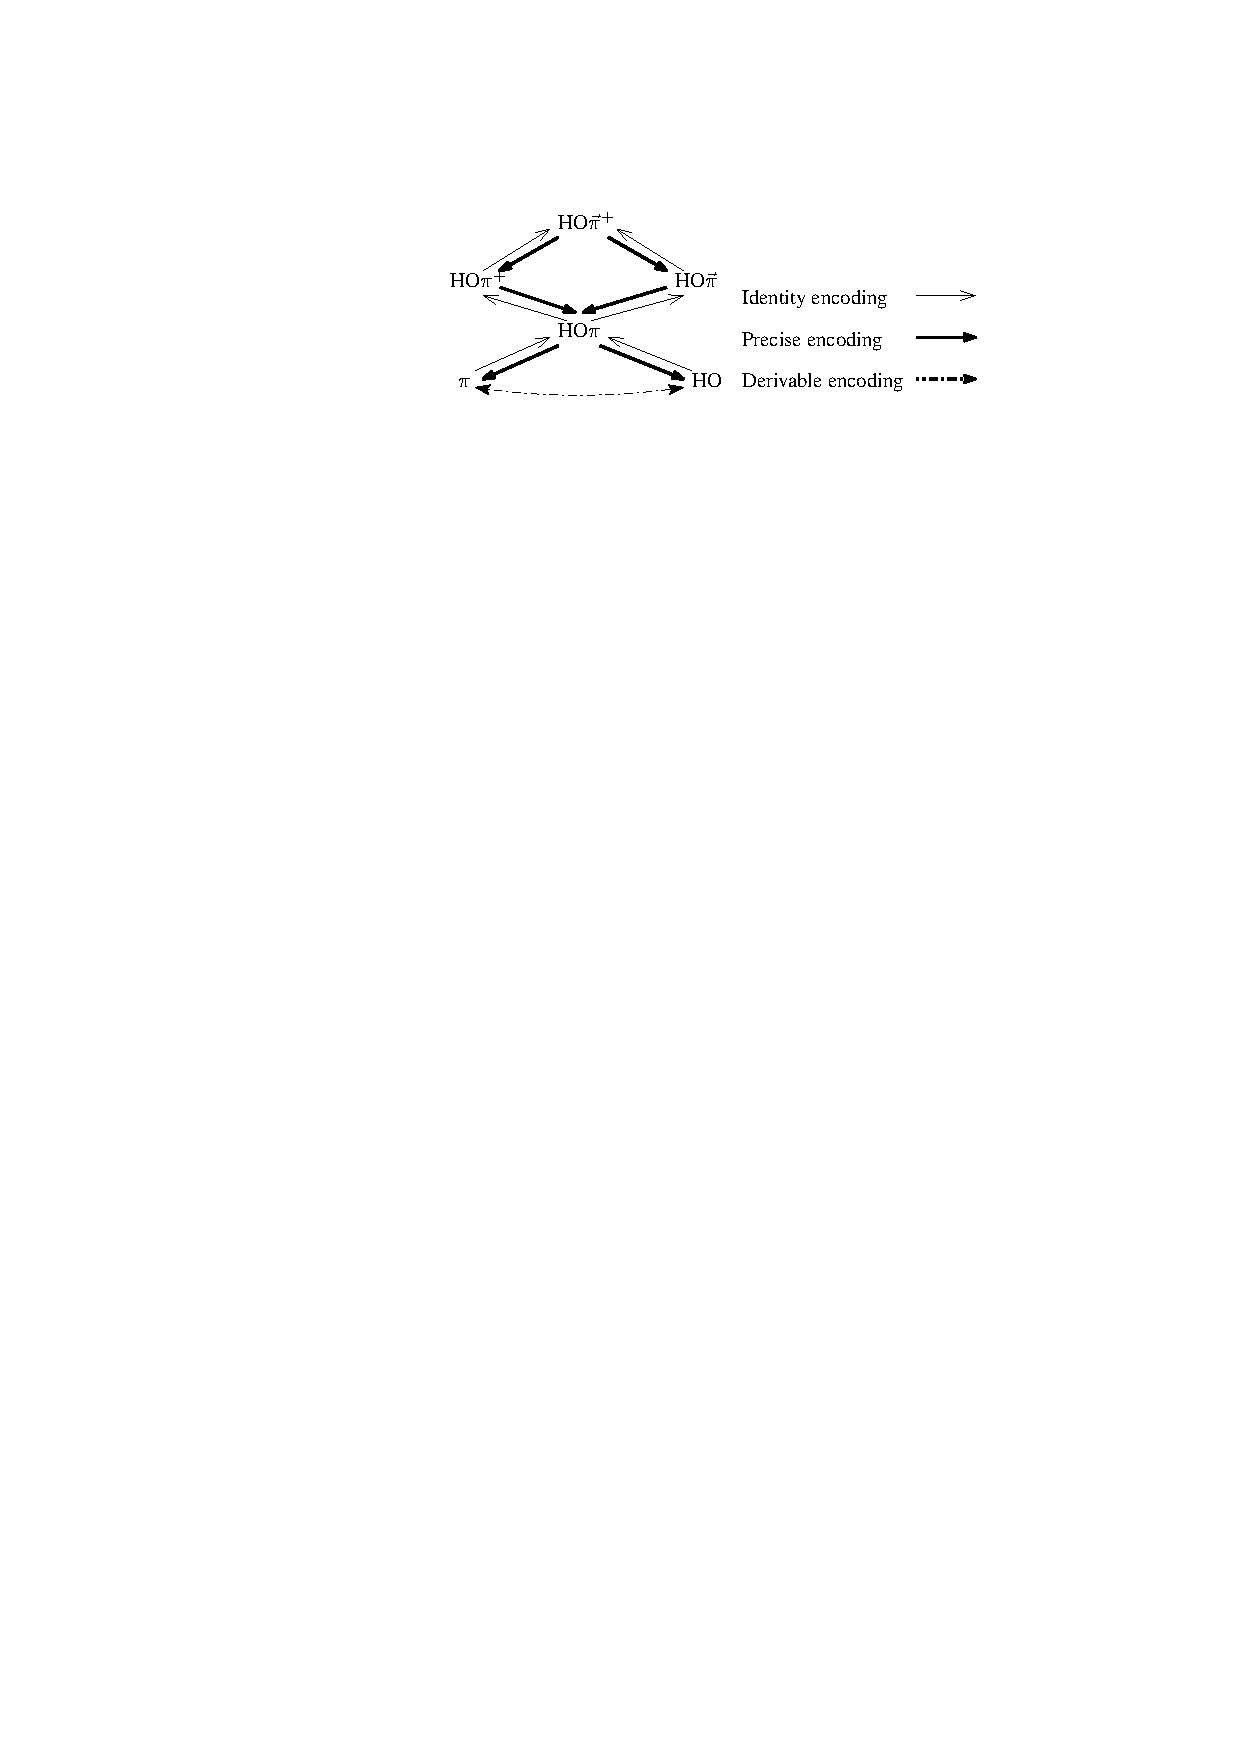
\includegraphics[scale=1]{diag.pdf}
\vspace{2mm}
%%ADD~FIGURE!
%	\centering
%	\begin{subfigure}[b]{0.45\linewidth}
%		\centering
%		\begin{tikzpicture}
%
%			\node	(PHOpp)	at	(0, 0.8)		{\PHOpp};
%			\node	(HOpp)	at	(-1.5, 0.4)	{\HOpp};
%			\node	(PHOp)	at	(1.5, 0.4)	{\PHOp};
%			\node	(HOp)	at	(0, 0)		{$\mathsf{HO}{\pi}^{~}$};
%			\node	(HO)	at	(-1.5, -0.4)	{$\mathsf{HO}{~}^{~}$};
%			\node	(sessp)	at	(1.5, -0.4)	{$~~\pi^{~}$};
%
%			\draw[<-]	(PHOpp) -- (HOpp);	%(0, 1.25) -- (-2, 1);
%			\draw[<-]	(PHOpp) -- (PHOp);	%(0, 1.25) -- (2, 1);
%
%			\draw[<-]	(HOpp) -- (HOp);	%(2, 0.5) -- (0, 0.25);
%			\draw[<-]	(PHOp) -- (HOp);	%(-2, 0.5) -- (0, 0.25);
%
%			\draw[<-]	(HOp) -- (HO);		%(0, -0.25) -- (-2, -0.5);
%			\draw[<-]	(HOp) -- (sessp);	%(0, -0.25) -- (2, -0.5);
%
%%				\node	(PHOpp)	at	(0, 0.8)		{\PHOpp};
%%				\node	(HOpp)	at	(-2, 0.4)	{\HOpp};
%%				\node	(PHOp)	at	(2, 0.4)	{\PHOp};
%%				\node	(HOp)	at	(0, 0)		{$\mathsf{HO}{\pi}^{~}$};
%%				\node	(HO)	at	(-2, -0.4)	{$\mathsf{HO}{~}^{~}$};
%%				\node	(sessp)	at	(2, -0.4)	{$~~\pi^{~}$};
%%
%%				\draw[->]	(PHOpp) -- (HOpp);	%(0, 1.25) -- (-2, 1);
%%				\draw[->]	(PHOpp) -- (PHOp);	%(0, 1.25) -- (2, 1);
%%
%%				\draw[->]	(HOpp) -- (HOp);	%(2, 0.5) -- (0, 0.25);
%%				\draw[->]	(PHOp) -- (HOp);	%(-2, 0.5) -- (0, 0.25);
%%
%%				\draw[->]	(HOp) -- (HO);		%(0, -0.25) -- (-2, -0.5);
%%				\draw[->]	(HOp) -- (sessp);	%(0, -0.25) -- (2, -0.5);
%		\end{tikzpicture}
%	\end{subfigure}
%%	\hfill
%	\begin{subfigure}[b]{0.5\linewidth}
%		\small
%		The arrow start calculus wrt arrow tip calculus:
%		\begin{itemize}
%			\item	is a sub-calculus.
%			\item	encodes.
%		\end{itemize}
%		Arrow properties are transitive.
%	\end{subfigure}
%\\
	\caption{Summary of Expressiveness Results. \label{fig:express}}
\Hlinefig
\end{figure}

\smallskip

\myparagraph{Outline / Contributions.} This paper 
is structured as follows:
\begin{enumerate}[$\bullet$]
\item \S\,\ref{sec:overview} overviews key ideas of our tractable bisimulations.
\item \S\,\ref{sec:calculus} presents the higher-order session calculus \HOp and its 
subcalculi \HO and \sessp.  Then, \S\,\ref{sec:types} gives the session type system
and states type soundness for \HOp and its variants.
\item \S\,\ref{sec:behavioural} 
develops \emph{higher-order} and \emph{characteristic} bisimilarities, our two
tractable characterisations of contextual equivalence which 
alleviate the issues of context bisimilarity~\cite{San96H}. These 
relations are shown to coincide in \HOp (Thm.~\ref{the:coincidence}).
\item \S\,\ref{s:expr} defines \emph{typed encodins} by extending encodability criteria 
proposed for
untyped processes~(e.g.~\cite{DBLP:journals/iandc/Gorla10,DBLP:conf/icalp/LanesePSS10}).
\item \S\,\ref{sec:positive} %and \S\,\ref{sec:negative}
gives encodings of \HOp into \HO and of \HOp into \sessp.
These encodings 
are shown to be \emph{precise} (Thms.~\ref{f:enc:hopitoho} and \ref{f:enc:hotopi}).
Mutual encodings between \sessp and \HO are derivable; 
all these calculi are thus equally expressive.
Exploiting determinacy and typed equivalences,
we also prove the non-encodability of shared names
into linear names (Thm.~\ref{t:negative}).

\item \S\,\ref{sec:extension} studies extensions of \HOp. We show that 
both \HOpp (the extension with higher-order applications) 
and \pHOp (the extension with polyadicity) are encodable in \HOp in a precise way
(Thms.~\ref{f:enc:hopiptohopi} and \ref{f:enc:phopiptohopi}).
These results connect our work with existing models of 
higher-order sessions~\cite{tlca07}.

\item \S\,\ref{sec:relwork} concludes with related works. An appendix summarises the typing system. 
\end{enumerate}
\noi
The paper is self-contained. 
{\bf\em Omitted definitions, additional related work, and  proofs 
%can be found
are 
in~\cite{KouzapasPY15}.} 



\section{Related Work}
\label{sec:relwork}
% !TEX root = main.tex
\myparagraph{Expressiveness.}
There is a vast literature on expressiveness studies for process calculi. 
For space reasons here we concentrate on closely related work; 
see~\cite{KouzapasPY15} for more detailed comparisons with other literature. 
%To formalise claims of (relative) expressiveness,
%%early works appealed to different definitions of encoding \cite{Palamidessi03}.
%%Later on, 
%abstract frameworks which define encodings and their 
%associated syntactic and semantic criteria 
%have been developed; 
%two proposals are~\cite{DBLP:journals/iandc/Gorla10,DBLP:journals/tcs/FuL10}. 
%These frameworks are applicable to different calculi, and 
%have shown useful to clarify known results and to derive new ones.
%Our formulation of (precise) typed encoding (\defref{def:goodenc}) 
%builds upon existing proposals (including~\cite{Palamidessi03,DBLP:journals/iandc/Gorla10,DBLP:conf/icalp/LanesePSS10})
%in order to account for the session type systems
%associated to \HOp and its variants/extensions.
%
%\myparagraph{Expressiveness of \emph{Higher-Order} Calculi.}
%Due to the close relationship between
%higher-order process calculi and functional calculi, works devoted to
%encoding (variants of) the $\lambda$-calculus into (variants of) the
%$\pi$-calculus~ (e.g.,~\cite{San92,DBLP:journals/tcs/Fu99}) are broadly related.
The encoding of process-passing into name-passing is well-known~\cite{SangiorgiD:expmpa};
an encoding in the reverse direction 
is given in~\cite{SaWabook} for an asynchronous, localised $\pi$-calculus
(only the output capability of names can be sent around).  The
work~\cite{San96int} studies hierarchies for calculi with
\emph{internal} first-order mobility and with higher-order mobility
without name-passing (like \HO). The
hierarchies are %based on expressivity: formally 
defined according to
the order of types needed in typing. 
%, they describe different ``degrees of mobility''.  
Via type-preserving fully abstract encodings, it is shown that 
name- and process-passing calculi with equal order of types have the
same expressiveness.  With respect to these previous results, our
approach based on session types has important consequences and
allows us to derive new results.  
Our study stresses the 
view of ``encodings as protocols'', namely session protocols which
enforce clean linear and shared disciplines for names, a distinction
not explored in~\cite{SangiorgiD:expmpa,DBLP:journals/tcs/Sangiorgi01}. In
turn, this distinction is central in proper definitions
of trigger processes, which are key to encodings
(\defref{d:enc:hopitopi}) and behavioural equivalences
(\defref{d:hbw} and~\ref{d:fwb}).  More interestingly, we showed that
$\HO$ suffices to encode  the session
calculus with name passing ($\sessp$) but also $\HOp$ and its extension with
higher-order applications ($\HOpp$). 
Thus, %using session types
all these session calculi are equally expressive with fully
abstract encodings.  To our knowledge, these are the first
expressivity results of this kind.

\jpc{Building upon~\cite{ThomsenB:plachoasgcfhop},
the work~\cite{XuActa2012} studies 
the (non)encodability of the $\pi$-calculus into 
a higher-order $\pi$-calculus with a powerful 
name relabelling operator, which is 
shown to be essential in encoding name-passing}. %, following \cite{Tho90}.
A core higher-order calculus is studied in~\cite{DBLP:journals/iandc/LanesePSS11}: 
it lacks restriction,  name passing, output prefix %(communication is asynchronous), 
and constructs for infinite behaviour. 
This calculus  has 
a simple notion of bisimilarity which coincides with 
%reduction-closed, barbed congruence.
contextual equivalence.
%be Turing complete, while 
%have a decidable notion of (strong) bisimilarity that coincides with barbed congruence. 
\jpc{
The absence of restriction plays a key role in the characterisations in~\cite{DBLP:journals/iandc/LanesePSS11};
hence, our characterisation of contextual equivalence for \HO (which has restriction)
cannot be derived from that in~\cite{DBLP:journals/iandc/LanesePSS11}. 
} 

%Our work is closely related in spirit to the expressiveness studies in~\cite{DBLP:conf/icalp/LanesePSS10,DBLP:conf/wsfm/XuYL13}.
In~\cite{DBLP:conf/icalp/LanesePSS10}
the core calculus in~\cite{DBLP:journals/iandc/LanesePSS11} is extended with restriction,
synchronous communication, and polyadicity. It is shown that 
synchronous communication can encode asynchronous communication, % (as in the first-order setting),
and that process passing polyadicity induces a hierarchy in expressive power.
Encodability criteria does not include full abstraction.
 % (unlike the first-order setting).
%A further extension with process abstractions of order one
%(functions from processes to processes)
% is shown to strictly add expressive power with respect to passing of processes only.
\jpc{The paper~\cite{DBLP:conf/wsfm/XuYL13} 
complements~\cite{DBLP:conf/icalp/LanesePSS10} 
by studying the expressivity %of second-order abstractions.
%with replication ($!P$).  
%The work \cite{DBLP:conf/wsfm/XuYL13} focuses  
%%name and process abstractions are distinguished and contrasted, also 
%on expressiveness of the hirarchy of polyadic abstraction parameters. 
%(the same kind of polyadicity present in \pHOp)
%By adapting the encodings in~\cite{DBLP:conf/icalp/LanesePSS10} 
%Polyadicity 
of 
second-order process abstractions.
Polyadicity is shown to induce an expressiveness hierarchy; 
also,
by adapting the encoding in~\cite{SangiorgiD:expmpa},
process abstractions are encoded into name abstractions.
In contrast, we 
give a fully abstract encoding of
 \PHOpp into \HO that preserves session types; this improves~\cite{DBLP:conf/icalp/LanesePSS10,DBLP:conf/wsfm/XuYL13}   
by enforcing linearity disciplines on process behaviour.
Also, the focus of~\cite{DBLP:conf/icalp/LanesePSS10,DBLP:conf/wsfm/XuYL13} is on 
the expressiveness of untyped, higher-order processes; they
%Moreover,~\cite{DBLP:conf/icalp/LanesePSS10,DBLP:conf/wsfm/XuYL13}
do not address 
tractable equivalences for processes  (such as 
$\hwb$ and $\fwb$) which only require observation of finite %number of 
%higher-order 
values,  
whose formulations rely on session types.}
%therefore, our work complements their  results. 
% by clarifying the status of typeful %, resource-aware 
%structured communications. % in trigger-based representations of process passing, both in encodings and  equivalences.

\myparagraph{Session Typed Processes.}
The works~\cite{DemangeonH11,Dardha:2012:STR:2370776.2370794} 
study encodings of binary session calculi into a linearly typed $\pi$-calculus. 
While~\cite{DemangeonH11}~gives a precise encoding of \sessp into a linear calculus 
(an extension of \cite{BHY}),  
the work~\cite{Dardha:2012:STR:2370776.2370794} 
gives operational correspondence (without full abstraction, cf.~\defref{def:sep}-4)
for the first- and higher-order 
$\pi$-calculi into \cite{LinearPi}. 
They investigate embeddability of two different typing systems;
by the result of \cite{DemangeonH11}, 
\HOpp is encodable  into the linearly typed $\pi$-calculi.     

The syntax of $\HOp$ is a subset of that in~\cite{tlca07,MostrousY15}.
The work~\cite{tlca07} develops a full higher-order session calculus
with process abstractions and applications; it admits the type 
$U=U_1 \rightarrow U_2 \dots U_n \rightarrow \Proc$ and its linear type 
$U^1$
which corresponds to $\shot{\tilde{U}}$ and $\lhot{\tilde{U}}$ in 
a super-calculus of $\HOpp$ and $\PHOp$. 
%in~\cite{MostrousY15} in the asynchronous setting.
%The session type
%system considered is influenced by the type systems for $\lambda$-calculi and
%uses type syntax of the form $U_1 \rightarrow U_2 \dots U_n \rightarrow \Proc$
%for shared values and $(U_1 \rightarrow U_2 \dots U_n \rightarrow \Proc)^{1}$
%for linear values.
%Such a type is expressed in $\HOpp$
%terms using the type $\shot{U}$ (respectively, $\lhot{U}$)
%with $U$ being a nested higher-order type; and 
%the $\HOp$ uses only types of the form
%$\shot{C}$ and $\lhot{C}$ with $C$ being a first-order channel type.
Our results show that
the calculus in~\cite{tlca07} is not only expressed but 
also reasoned in 
$\HO$ (with limited form of arrow types, $\shot{C}$ and $\lhot{C}$), via precise encodings. \dk{None of the above works proposes tractable 
bisimulations for higher-order processes.}  

\myparagraph{Typed Behavioural Equivalences.}
\NY{This work follows 
the 
%principles for
session type behavioural semantics in 
\cite{KYHH2015,KY2015,DBLP:journals/iandc/PerezCPT14}
where a bisimulation is defined on a LTS 
that assumes a session typed
observer.
%The bisimilarity is characterised by the corresponding
%reduction-closed, barbed congruence using techniques derived from~\cite{Hennessy07}.
Our theory for higher-order session types 
differentiates from 
the work in~\cite{KYHH2015,KY2015}, which 
considers the first-order
binary and multiparty session types, respectively.
The work \cite{DBLP:journals/iandc/PerezCPT14} gives a behavioural theory 
for a 
logically motivated
language of binary sessions 
without shared names.}
%Determinacy properties (confluence, $\tau$-inertness) are proven.

%The theory for higher-order session type quivalences is more challenging than
%their corresponding first-order bisimulation theory.
Our approach %for the higher-order 
to typed equivalences
builds upon techniques by Sangiorgi~\cite{SangiorgiD:expmpa,San96H}
and Jeffrey and Rathke~\cite{JeffreyR05}.
The work %Sangiorgi as part of his Ph.D.~research
%\cite{San96H,SangiorgiD:expmpa}
\cite{SangiorgiD:expmpa}
introduced the first fully-abstract encoding from the higher-order 
$\pi$-calculus into the $\pi$-calculus. 
Sangiorgi's encoding is based on the idea of a replicated input-guarded process 
(a trigger process). We use a similar 
replicated triggered process 
to encode \HOp into \sessp (\defref{d:enc:hopitopi}).
 Operational correspondence for
the triggered encoding is shown using a context bisimulation
with first-order labels.
%Although contextual bisimilarity has a satisfactory discriminative power,
%its use is hindered by the universal quantification on output clauses.
To deal with the issue of context biimilarity, 
Sangiorgi proposes \emph{normal bisimilarity}, 
a tractable  equivalence without universal quantification. 
To prove that context and normal bisimilarities coincide,~\cite{SangiorgiD:expmpa} uses 
triggered processes.
%The encoding also motivates the definition of a form of
Triggered bisimulation is also defined on first-order labels
where the context bisimulation is restricted to arbitrary
trigger substitution. %rather than arbitrary process substitutions.
This
characterisation of context bisimilarity  was refined in~\cite{JeffreyR05} for
calculi with recursive types, not addressed in~\cite{San96H,SangiorgiD:expmpa} and
relevant in our work (cf. \defref{d:enc:hopitoho}).
The
bisimulation in~\cite{JeffreyR05}
is based on an LTS which is extended with trigger meta-notation.
%for a full higher-order $\pi$-calculus that allows
%higher-order applications.
As in~\cite{San96H,SangiorgiD:expmpa}, 
the LTS in~\cite{JeffreyR05}
observes first-order triggered values instead of
higher-order values, offering a more direct characterisation of contextual equivalence
and lifting the restriction to finite types.
We briefly contrast 
the approach in~\cite{JeffreyR05} and ours based on 
\dk{higher-order ($\hwb$) and} characteristic ($\fwb$) bisimilarities:
\begin{enumerate}[$\bullet$]
%\begin{enumerate}[i.]
\item 
The LTS in~\cite{JeffreyR05} is enriched with extra labels for triggers;
an output action transition emits a trigger and introduces a parallel replicated trigger.
Our 
approach retains usual labels/transitions; in  case of output,
%our bisimilarities 
$\hwb$ and $\fwb$
introduce a parallel
non-replicated trigger.
\item Higher-order input in~\cite{JeffreyR05} involves 
the input of a trigger which reduces after substitution.
Rather than a trigger name, %our bisimulations  
$\hwb$ and $\fwb$
decree the input of a triggered value $\abs{z}\binp{t}{x} \appl{x}{z}$.
\item Unlike~\cite{JeffreyR05}, 
%our 
$\fwb$ treats  
first- and higher-order values uniformly. In the latter case, 
since the typed LTS distinguishes between linear and shared values, 
replicated closures are used only for shared values.

\item In~\cite{JeffreyR05} a matching construct is
crucial to prove completeness of bisimilarity,
while our calculi lack matching. 
%Contrarily 
\jpc{In contrast,} 
we use the characteristic
process interaction with the environment, exploiting 
session type structures, i.e., instead of matching 
a name is embedded into a process and then observe its behaviour.

%In~\cite{JeffreyR05}  a matching construct 
%is crucial to prove completeness of bisimilarity.
%Since our language lacks matching,
%we use session type information to obtain the simplest value that 
%enables interaction with the environment.

\end{enumerate}

%There are similarities and differences between of the characteristic bisimulation
%and the bisimulation as defined by Jeffrey and Rathke
%(below we use the meta-notation adopted in~\cite{JeffreyR05}):
%%
%\begin{enumerate}[i)]
%	\item	The output of a higher-order value $\abs{x}{Q}$ on name
%		$n$ in Jeffrey\&Rathke approach requires the output of
%		a fresh trigger name $t$ (notation $\tau_t$)
%		on name $n$ 
%		and then the introduction of a replicated triggered process
%		(notation $(t \Leftarrow (x) Q)$)
%		in the context of the acting process:
%		%
%		\[
%			P \by{\news{t} \bactout{n}{\tau_{t}}} P' \Par (t \Leftarrow (x) Q) \by{\bactinp{t}{v}} P' \Par \appl{(x) Q}{v} \Par (t \Leftarrow (x) Q) 
%		\]
%		%
%		In the characteristic bisimulation approach we only observe
%		an output of a value that can be either first- or higher-order:
%		%
%		\[
%			P \hby{\bactout{n}{V}} P' 
%		\]
%		%
%		with $V = \abs{x}{Q}$ or $V = m$.
%		A non-replicated triggered process appears in
%		the parallel context of the acting process when
%		we compare two processes for behavioural equality
%		(cf.~characteristic bisimulation \defref{d:fwb}),
%		$P' \Par \htrigger{t}{\abs{x}{Q}}$.
%		In fact using the LTS in
%		\defref{d:tlts} we can get:
%		%
%		\begin{eqnarray*}
%			P' \Par \htrigger{t}{\abs{x}{Q}}
%			&\by{\abs{z}{\binp{z}{y} \repl{} \binp{t}{x} \appl{y}{x}}}&
%			P' \Par \newsp{s}{\binp{s}{y} \repl{} \binp{t}{x} \appl{y}{x} \Par \bout{s}{\abs{x}{Q}} \inact}\\
%			&\by{\tau}&
%			P' \Par \repl{}\binp{t}{y} \appl{\abs{x}{Q}}{y}
%		\end{eqnarray*}
%		%
%		that simulates the Jeffrey\&Rathke approach.
%
%		The characteristic bisimulation differentiates from
%		the Jeffrey\&Rathke approach:
%		\begin{enumerate}[$\bullet$]
%			\item	The typed LTS predicts the case of linear
%				output values and will never allow replication
%				of such a value;
%				if $V$ is linear the input action would have no replication
%				operator, as
%				$\abs{z}{\binp{z}{y} \binp{t}{x} \appl{y}{x}}$.
%
%			\item	The characteristic bisimulation introduces a uniform approach
%				not only for
%				higher-order values but for first-order values
%				as well. A triggered process can accept any
%				process that can substitute a first-order value as well.
%				This is derived from the fact that the $\HOp$
%				calculus makes no use of a matching operator, in contrast
%				to the calculus defined in~\cite{JeffreyR05})
%				where name matching is crucial to prove completness
%				of the bisimilarity relation.
%				We chose not to include the matching operator
%				because of the requirement of a minimal calculus.
%				In the lack of matching we use types to inhabit
%				a value so we can observe its simplest interaction
%				with the process environment.
%
%			\item	The \HOp calculus requires only first-order
%				applications. Higher-order applications,
%				as in the Jeffrey\&Rathke work,
%				are presented as an extension in the \HOpp
%				calculus.
%
%			\item	The trigger process is non-replicated. In fact
%				the trigger process transforms guards the output
%				value with a higher-order input prefix. The
%				functionality of the input is used to
%				simulate the contextual bisimilarity that subsumes
%				the replicated trigger approach.
%				The transformation of an output action as an input
%				action allows for treating an output
%				using the restricted LTS \defref{def:rlts}:
%				%
%				\[
%					P' \Par \htrigger{t}{\abs{x}{Q}} \hby{\bactinp{t}{\abs{x}{\mapchar{U}{x}}}}
%					P' \Par \news{s}{ \appl{\mapchar{U}{x}}{s} \Par \bout{\dual{s}}{\abs{x}{Q}} \inact}
%				\]
%		\end{enumerate}
%		%
%		%In essence we are transforming a replicated trigger into a process
%		%that is input-prefixed on a fresh name that receives a higher-order
%		%value;
%
%	\item	The input of a higher-order value in the Jeffrey\&Rathke approach requires 
%		the input of a fresh trigger name, which is substituted on the application
%		variable, thus having a meta-suntax for triggered application instead
%		of higher-order applications:
%		%
%		\[
%			\binp{n}{x} P \by{\bactinp{n}{\tau_k}} \appl{\abs{x}{P}}{\tau_k} \by{\tau} P \subst{x}{\tau_k} 
%		\]
%		%
%		with every instance of process variable $x$ in $P$ being substituted
%		with trigger value $\tau_k$ to give a process of the form $\appl{\tau_k}{x}$.
%		The approach in the characteristic bisimulation observes the
%		triggered value
%		$\abs{z}\binp{t}{x} \appl{x}{z}$ as an input instead of the
%		trigger name:
%		%
%		\[
%			P \hby{\bactinp{n}{\abs{z}\binp{t}{x} \appl{x}{z}}} P \subst{\abs{z}\binp{t}{x} \appl{x}{z}}{x}
%		\]
%		%
%		with applications being transformed to
%		$\abs{z}{\binp{t}{x} \appl{x}{z}}{v}$
%		Note that in the characteristic bisimulation semantics
%		we can also observe a characteristic process as an input.
%		
%	\item 	Triggered application in the Jeffrey\&Rahtke
%		are observe using an output
%		lead into an output observation of the
%		application value over
%		the fresh trigger name.
%		%
%		\[
%			\appl{\tau_k}{v} \by{\bactout{k}{v}} \inact
%		\]
%		%
%		In the characteristic bisimulation instead of observing an 
%		application and its value as an action we observe:
%		i) the name of the trigger through the trigger value
%		application; and ii) the application
%		value by inhabiting it in the characteristic value
%		and observing the interaction of the corresponding
%		characteristic process with its environment.
%		%
%		\begin{eqnarray*}
%			\appl{\abs{z}{\binp{t}{x} \appl{x}{z}}}{v} &\by{\tau}& \binp{t}{x} \appl{x}{v}
%			\by{\bactinp{t}{\abs{x}{\mapchar{U}{x}}}}
%			\appl{\abs{x}{\mapchar{U}{x}}}{v}
%			\by{\tau} \mapchar{U}{x} \subst{n}{x}
%		\end{eqnarray*}
%		%
%\end{enumerate}

%The main differences of the triggered
%bisimulation approach comparing to our approach are:
%i) We use observe higher-order values on the LTS in contrast to first-order 
%values in~\cite{DBLP:journals/lmcs/JeffreyR05}.
%ii) In our approach we avoid the replicated triggered process,
%by transforming the output process into a higher-order guarded input.
%iii) The triggered bisimulation gives semantics for higher-order application,
%whereas in our approach we give semantics for first-order applications
%and show that higher-order applications are fully encodable.

%Boreale and Sangiorgi, 
%Deng and Hennessy, 
%Jeffrey and Rathke, Hennessy and Koutavas, Schmitt and Lenglet, Pi\E9rard and Sumii.
%Perez et al (bisimilarities for binary sessions), Kouzapas and Yoshida (bisimilarities for binary and multiparty sessions).
%Bisimilarities for HO processes: \cite{Xu07}.

\noi 
The work~\cite{DBLP:conf/lics/SangiorgiKS07} defines \emph{environmental bisimulations},
which 
%Sangiorgi et al.~\cite{DBLP:conf/lics/SangiorgiKS07}, 
use a higher-order LTS 
to define a bisimulation that stores the knowledge known to
the observer; hence, observed actions are based on the observer's knowledge
at any given time. This approach is enhanced in~\cite{DBLP:journals/cl/KoutavasH12,DBLP:conf/esop/KoutavasH11}
where a mapping from constants to higher-order values is introduced. This 
allows to observe first-order values instead
of higher-order values. It differs from~\cite{San96H,JeffreyR05} in that 
the mapping between higher- and first-order values is no longer implicit.







\section{Higher-Order Session $\pi$-Calculi}
\label{sec:calculus}
% !TEX root = main.tex
\noindent 
We introduce the 
\emph{Higher-Order Session $\pi$-Calculus} (\HOp).
\HOp includes both name- and abstraction-passing 
as well as recursion; it is a subcalculus 
of the language
studied 
in~\cite{tlca07}. 
Following the literature~\cite{JeffreyR05},
for simplicity of the presentation
we concentrate on the second-order call-by-value \HOp.  
(In \secref{sec:extension} we consider extensions of 
\HOp with higher-order abstractions 
and polyadicity in name-passing/abstractions.)
%We also introduce two subcalculi of \HOp. In particular, we define the 
%core higher-order session
%calculus (\HO), which 
%%. The \HO calculus is  minimal: it 
%includes constructs for shared name synchronisation and 
%%constructs for session establish\-ment/communication and 
%(monadic) name-abstraction, but lacks name-passing and recursion.

%Although minimal, in \secref{s:expr}
%the abstraction-passing capabilities of \HOp will prove 
%expressive enough to capture key features of session communication, 
%such as delegation and recursion.

\subsection{Syntax of \HOp}
\label{subsec:syntax}
\noindent\myparagraph{Values} The syntax of \HOp is defined in \figref{fig:syntax}
\begin{figure}[t]
\[ 
\begin{array}{lll}
u,w  ::=  n \ | \ x,y,z
& n ::= a,b  \ | \ s, \dual{s} 
& V,W  ::=   \nonhosyntax{u} \ | \ \abs{x}{P}
\end{array}
\]
\[
\begin{array}{rclllll}
P,Q \!\!\!\!\!\! & ::= & \!\! \bout{u}{V}{P}  \bnfbar  \binp{u}{x}{P} \bnfbar
 \bsel{u}{l} P \bnfbar \bbra{u}{l_i:P_i}_{i \in I}   \\[1mm]
 & \bnfbar & \!\!  \nonhosyntax{\rvar{X} \bnfbar \recp{X}{P}} \bnfbar \appl{V}{u} \bnfbar P\Par Q \bnfbar \news{n} P 
\bnfbar 
%ny
%\appl{x}{u}

 \inact
%\\[1mm]
 %    & \bnfbar & \nonhosyntax{\rvar{X} \bnfbar \recp{X}{P}}
\end{array}
\]
 \caption{Syntax of \HOp (\HO lacks the constructs in \nonhosyntax{\text{grey}}).}
\label{fig:syntax}
\Hlinefig
\end{figure}
We use $a,b,c, \dots$ (resp.~$s, \dual{s}, \dots$) 
to range over shared (resp. session) names. 
We use $m, n, t, \dots$ for session or shared names. 
We define the dual operation over names $n$ as $\dual{n}$ with
$\dual{\dual{s}} = s$ and $\dual{a} = a$.
Intuitively, names $s$ and $\dual{s}$ are dual (two) \emph{endpoints} while 
shared names represent shared (non-deterministic) points. 
Variables are denoted with $x, y, z, \dots$, 
and recursive variables are denoted with $\varp{X}, \varp{Y} \dots$.
An abstraction %(or higher-order value) 
$\abs{x}{P}$ is a process $P$ with name parameter $x$.
%Symbols $u, v, \dots$ range over identifiers; and  $V, W, \dots$ to denote values. 
Values $V,W$ include 
identifiers $u, v, \ldots$ %(first-order values) 
and 
abstractions $\abs{x}{P}$ (first- and higher-order values, resp.). 

\myparagraph{Terms} 
include the
$\pi$-calculus prefixes for sending and receiving values $V$.
Process $\bout{u}{V} P$ denotes the output of value $V$
over name $u$, with continuation $P$;
process $\binp{u}{x} P$ denotes the input prefix on name $u$ of a value
that 
will substitute variable $x$ in continuation $P$. 
Recursion is expressed by $\recp{X}{P}$,
which binds the recursive variable $\varp{X}$ in process $P$.
Process 
%ny
%$\appl{x}{u}$ 
$\appl{V}{u}$ 
is the application
which substitutes name $u$ on the abstraction~$V$. 
\dk{Typing  ensures \jpc{that} $V$ is not a name.}
Prefix $\bsel{u}{l} P$ selects label $l$ on name $u$ and then behaves as $P$.
%Given $i \in I$ 
Process $\bbra{u}{l_i: P_i}_{i \in I}$ offers a choice on labels $l_i$ with
continuation $P_i$, given that $i \in I$.
%Others are standard c
Constructs for 
inaction $\inact$,  parallel composition $P_1 \Par P_2$, and 
name restriction $\news{n} P$ are standard.
Session name restriction $\news{s} P$ simultaneously binds endpoints $s$ and $\dual{s}$ in $P$.
%A well-formed process relies on assumptions for
%guarded recursive processes.
We use $\fv{P}$ and $\fn{P}$ to denote a set of free 
%\jpc{recursion}
variables and names; 
and assume $V$ in $\bout{u}{V}{P}$ does not include free recursive 
variables $\rvar{X}$. 
If $\fv{P} = \emptyset$, we call $P$ {\em closed}.
%; and closed $P$ without 
%free session names a {\em program}. 

\subsection{Subcalculi of \HOp}
\label{subsec:subcalculi}
\noi
We define two subcalculi of \HOp. 
%We now define several sub-calculi of \HOp. 
The first is the 
{\em core higher-order session calculus} (denoted \HO),
which lacks recursion and name passing; its 
formal syntax is obtained from \figref{fig:syntax} by excluding 
constructs in \nonhosyntax{\text{grey}}.
The second subcalculus is 
the {\em session $\pi$-calculus} 
(denoted $\sessp$), which 
lacks  the
higher-order constructs
(i.e., abstraction passing and application), but includes recursion.
Let $\CAL \in \{\HOp, \HO, \sessp\}$. We write 
$\CAL^{-\mathsf{sh}}$ for $\CAL$ without shared names
(we delete $a,b$ from $n$). 
We shall demonstrate that 
$\HOp$, $\HO$, and $\sessp$ have the same expressivity.

\subsection{Operational Semantics}
\label{subsec:semantics}
\begin{figure}
\[
\begin{array}{rclrcrclr}
(\abs{x}{P}) \, u  & \red & P \subst{u}{x} 
& \orule{App}
		\\[1mm]
%\bout{a}{V} P \Par \binp{a}{x} Q & \red & P \Par Q \subst{V}{x} 
%& \orule{Com}
%		\\[1mm]
\bout{n}{V} P \Par \binp{\dual{n}}{x} Q & \red & P \Par Q \subst{V}{x} 
& \orule{Pass}
		\\[1mm]
		\bsel{n}{l_j} Q \Par \bbra{\dual{n}}{l_i : P_i}_{i \in I} & \red & Q \Par P_j ~~(j \in I)~~  & \orule{Sel}\\[1mm]
		P \red P' & \Rightarrow & \news{n} P  \red  \news{n} P'  & \orule{Res}\\[1mm]
			P \red P' & \Rightarrow  &  P \Par Q  \red   P' \Par Q  & \orule{Par}\\[1mm]
			P \scong Q \red Q' \scong P' & \Rightarrow & P  \red  P' & \orule{Cong}
	\end{array}
\]
{\small
\[
	\begin{array}{c}
		P \Par \inact \scong P
		\quad
		P_1 \Par P_2 \scong P_2 \Par P_1
		\quad
		P_1 \Par (P_2 \Par P_3) \scong (P_1 \Par P_2) \Par P_3
		%\quad
		%P \scong Q \textrm{ if } P \scong_\alpha Q
		\\[1mm]
		\news{n} \inact \scong \inact
		\quad 
		P \Par \news{n} Q \scong \news{n}(P \Par Q)
		\	(n \notin \fn{P})\quad 
		\recp{X}{P} \scong P\subst{\recp{X}{P}}{\rvar{X}}
		\\[1mm]
		P \scong Q \textrm{ if } P \scong_\alpha Q
%		\qquad
%		\dk{V \scong W \textrm{ if } V \scong_\alpha W
%\quad \abs{x}{P} \scong \abs{x}{Q} \textrm{ if } P \scong Q}
	\end{array}
\]
}
\caption{Operational Semantics of $\HOp$. 
\label{fig:reduction}}
\Hlinefig
\end{figure}
\noindent \figref{fig:reduction} defines the operational semantics 
of \HOp.
$\orule{App}$ is a name application; 
$\orule{Pass}$ defines a shared interaction at $n$ 
(\jpc{with} $\dual{n}=n$) or a session interaction;  
$\orule{Sel}$ is the standard rule for labelled choice/selection:
given an index set $I$, 
a process selects label $l_j$ on name $n$ over a set of
labels $\set{l_i}_{i \in I}$ offered by a branching 
on the dual endpoint $\dual{n}$; and other rules are standard.
Rules for \emph{structural congruence} are defined in \figref{fig:reduction} (bottom). 
\jpc{We assume the expected extension of $\scong$ to values $V$.}
We write $\red^\ast$ for a multi-step reduction. 


\section{Types and Typing}
\label{sec:types}
\section{Types for $\HOp$}

We define a session type system for $\HOp$, which is based on the type system developed by Mostrous
and Yoshida in~\cite{tlca07}.

\subsection{Session Types}
We consider a minimal type structure, a fragment of that defined in~\cite{tlca07}.
The only (but fundamental) differences are in the types for values: we focus on having 
$\shot{S}$ and $\lhot{S}$, whereas the structure in~\cite{tlca07} supports general functions $U \sharedop T$ and 
$U \lollipop T$.
\[
	\begin{array}{lcl}
		\text{\emph{Values}} & U ::= & S \bnfbar \lhot{S} \bnfbar \shot{S} \bnfbar \chtype{S} \qquad \quad \text{\emph{Terms}} \quad T ::= U  \bnfbar  \Proc\\
		\text{\emph{Sessions}} \ & S ::= &  \btout{U} S \bnfbar \btinp{U} S
		\bnfbar		\btsel{l_i:S_i}_{i \in I} \bnfbar \btbra{l_i:S_i}_{i \in I} \bnfbar \trec{t}{S} \bnfbar \vart{t}  \bnfbar \tinact 
	\end{array}
\]

There are four different value types $U$; session value $S$, linear higher order value $\lhot{S}$, 
shared higher order value $\shot{S}$; shared channel $\chtype{S}$. Terms can either have a
value type $U$ or a process type $\Proc$.

Session types follow the standard binary session types syntax \cite{}. Session send prefix $\btout{U} S$ 
denotes a session type that sends a value of type $U$ and continues as $S$. Dually receive prefix $\btinp{U} S$
denotes a session type that receives a value of type $U$ and continues as $S$. 
Set $\mathsf{ST}$ is the space of all session types.

\begin{definition}[Duality]
	Let function $F(R): \mathsf{ST} \longrightarrow \mathsf{ST}$ to be defined as:

	\begin{tabular}{rcl}
		$F(R)$ &$=$&		$\set{(\tinact, \tinact), (\vart{t}, \vart{t})}$\\
			&$\cup$&	$\set{(\btout{U};S_1, \btinp{U}; S_2), (\btinp{U};S_1, \btout{U}; S_2) \bnfbar S_1\ R\ S_2}$\\
			&$\cup$&	$\set{(\btsel{l_i: S_i}_{i \in I}, \btbra{l_j: S_j'}_{j \in J}) \bnfbar I \subseteq J, S_i\ R\ S_j'}$\\
			&$\cup$&	$\set{(\btbra{l_i: S_i}_{i \in I}, \btsel{l_j: S_j'}_{j \in J}) \bnfbar J \subseteq I, S_j\ R\ S_i'}$\\
			&$\cup$&	$\set{(\trec{t}{S_1}, \trec{t}{S_2}) \cup (S_1 \subst{\trec{t}{S}}{\vart{t}}, S_2), (S_1, S_2\subst{\trec{t}{S}}{\vart{t}}) \bnfbar S_1\ R\ S_2)}$
	\end{tabular}

	Standard arguments ensure that $F$ is monotone, thus the greatest fix point
	of $F$ exists and let duality defined as $\dualof = \nu X. F(X)$.
\end{definition}


Following our decision of focusing on functions $\shot{S}$ and $\lhot{S}$,
our environments are also simpler than those in~\cite{tlca07}:
\[
	\begin{array}{lcl}
		\text{Shared} & \Gamma \bnfis & \emptyset \bnfbar \Gamma \cat \varp{X}: \shot{S} \bnfbar \Gamma \cat k: \chtype{S} \bnfbar \Gamma \cat \rvar{X}: \Sigma \\
		\text{Linear} & \Lambda \bnfis & \emptyset \bnfbar \Lambda \cat \varp{X}: \lhot{S}  \\
		\text{Session} \quad & \Sigma \bnfis & \emptyset \bnfbar \Sigma \cat k:S  
	\end{array}
\]


With these environments the shape of judgments is exactly the same as in Mostrous and Yoshida's system:
\[
	\begin{array}{c}
		\Gamma; \Lambda ; \Sigma \proves P \hastype T
%		\Gamma; \Lambda; \Sigma \proves V \hastype U
	\end{array}
\]
As expected, weakening, contraction, and exchange principles apply to $\Gamma$;
environments $\Lambda$ and $\Sigma$ behave linearly, and are only subject to exchange.
We require that the domains of $\Gamma, \Lambda$ and $\Sigma$ are pairwise distinct.
%We focus on \emph{well-formed} judgments, which do not share elements in their domains.
%\newcommand{\jrule}[3]{\displaystyle \frac{#1 }{#2} & \trule{#3}}
\newcommand{\jrule}[3]{\displaystyle \trule{#3}~~\frac{#1 }{#2}}
\newcommand{\addenv}{\circ}

\begin{figure}[!t]
\[
	\begin{array}{c}
%		\jrule{ }{\Gamma ; \emptyset; \emptyset \vdash \UnitV \hastype \Unit}{Unit} 
%		\qquad\quad  
		\trule{Session}~~\Gamma; \emptyset; \set{k:S} \proves k \hastype S 
		\\[2mm]
		\trule{Shared}~~\Gamma \cat a : \chtype{S}; \emptyset; \emptyset \proves a \hastype \chtype{S}
		\qquad
		\trule{LVar}~~\Gamma; \set{X: \lhot{S}}; \emptyset \proves X \hastype \lhot{S} 
		\\[2mm]
		\trule{Prom}~~\tree{
			\Gamma; \emptyset; \emptyset \proves V \hastype \lhot{S}
		}{
			\Gamma; \emptyset; \emptyset \proves V \hastype \shot{S}
		} 
		\qquad\quad  
		\trule{Derelic}~~\tree{
			\Gamma; \Lambda \cat X{:}\lhot{S}; \Sigma \proves P \hastype \Proc
		}{
			\Gamma \cat X:\shot{S}; \Lambda; \Sigma \proves P \hastype \Proc
		} 
		\\[4mm]
%		\trule{Subt}~~\tree{
%			\Gamma; \Lambda; \Sigma \proves P \hastype T \quad \Sigma \subt \Sigma' \quad T \subt T'
%		}{
%			\Gamma ; \Lambda; \Sigma' \vdash P \hastype T'
%		} 
%		\qquad\quad

		\trule{Abs}~~\tree{
			\Gamma; \Lambda; \Sigma \cat x: S \proves P \hastype \Proc
		}{
			\Gamma; \Lambda; \Sigma \proves \abs{x}{P} \hastype \lhot{S}
		}
		\\[4mm]

		\trule{App}~~\tree{(U = \lhot{S}) \lor (U = \shot{S}) \quad \Gamma; \Lambda_1; \Sigma_1 \proves X \hastype U  \quad \Gamma; \Lambda_2; \Sigma_2 \proves k \hastype S
		}{
			\Gamma; \Lambda_1 \cup \Lambda_2; \Sigma_1 \cup \Sigma_2 \proves \appl{X}{k} \hastype \Proc
		} 
		\\[4mm]

		\trule{Send}~~\tree{
			\Gamma; \Lambda_1; \Sigma_1 \proves P \hastype \Proc  \quad \Gamma; \Lambda_2; \Sigma_2 \vdash V \hastype U  \quad (k:S \in \Sigma_1 \cup \Sigma_2)
		}{
			\Gamma; \Lambda_1 \cup \Lambda_2; (\Sigma_1 \cup \Sigma_2)\backslash\set{k:S} \cat k:\btout{U} S \proves \bout{k}{V} P \hastype \Proc
		}

		\\[4mm]
		\trule{Conn}~~\tree{
			\Gamma; \Lambda; \Sigma \cat x:S \proves P \hastype \Proc  \quad \Gamma; \emptyset; \emptyset \proves a \hastype \chtype{S}
		}{
			\Gamma; \Lambda; \Sigma \proves \binp{a}{x} P \hastype \Proc
		}
		\\[4mm]
%		\trule{ConnDual}~~\tree{
%			\Gamma; \Lambda; \Sigma \cat x: S_1 \proves P \hastype \Proc  \quad \Gamma; \emptyset; \emptyset \proves k \hastype \chtype{S_2} \quad S_1 \dualof S_2
%		}{
%			\Gamma; \Lambda; \Sigma \proves \bout{k}{x} P \hastype \Proc
%		}
%		\\[4mm]

		\trule{ConnDual}~~\tree{
			\Gamma; \Lambda; \Sigma \cat \dual{s}: S_1 \proves P \hastype \Proc  \quad \Gamma; \emptyset; \emptyset \proves a \hastype \chtype{S_2} \quad S_1 \dualof S_2
		}{
			\Gamma; \Lambda; \Sigma  \proves \bout{a}{\dual{s}} P \hastype \Proc
		}

		\\[4mm]

		\trule{NewSh}~~\tree{
			\Gamma\cat a:\chtype{S} ; \Lambda; \Sigma \proves P \hastype \Proc
		}{
			\Gamma; \Lambda; \Sigma \proves \news{a} P \hastype \Proc}
		\qquad\quad
		\trule{NewSes}~~\tree{
			\Gamma; \Lambda; \Sigma \cat s:S_1 \cat \dual{s}: S_2 \proves P \hastype \Proc \quad S_1 \dualof S_2
		}{
			\Gamma; \Lambda; \Sigma \proves \news{s} P \hastype \Proc
		}
		\\[4mm]

		\trule{RecvS}~~\tree{
			\Gamma; \Lambda; \Sigma \cat k: S_1 \cat x: S_2 \proves P \hastype \Proc
		}{
			\Gamma; \Lambda; \Sigma, k: \btinp{S_2} S_1  \vdash \binp{k}{x}P \hastype \Proc
		}
		\quad\quad 
		\trule{RecvL}~~\tree{
			\Gamma; \Lambda \cat X: \lhot{S}; \Sigma \cat k: S_1  \proves P \hastype \Proc
		}{
			\Gamma; \Lambda; \Sigma \cat k:\btinp{\lhot{S}}S_1  \proves \binp{k}{X}P \hastype \Proc
		}
		\\[4mm]

		\trule{RecvSh}~~\tree{
			\Gamma \cat X: \shot{S}; \Lambda; \Sigma \cat k: S_1  \proves P \hastype \Proc
		}{
			\Gamma; \Lambda; \Sigma \cat k:\btinp{\shot{S}}S_1  \proves \binp{k}{X}P \hastype \Proc
		}
		\quad ~~
		\trule{RecvShN}~~\tree{
			\Gamma \cat x: \chtype{S}; \Lambda; \Sigma \cat k: S_1  \proves P \hastype \Proc
		}{
			\Gamma; \Lambda; \Sigma \cat k:\btinp{\chtype{S}}S_1  \proves \binp{k}{x}P \hastype \Proc
		}
		\\[4mm]
		\trule{Par}~~\tree{
			\Gamma; \Lambda_{1}; \Sigma_{1} \proves P_{1} \hastype \Proc \quad \Gamma; \Lambda_{2}; \Sigma_{2} \proves P_{2} \hastype \Proc
		}{
			\Gamma; \Lambda_{1} \cup \Lambda_2; \Sigma_{1} \cup \Sigma_2 \proves P_1 \Par P_2 \hastype \Proc
		}
		\qquad\quad
		\trule{Close}~~\tree{
			\Gamma; \Lambda; \Sigma  \proves P \hastype T \quad k \not\in \dom{\Gamma, \Lambda,\Sigma}
		}{
			\Gamma; \Lambda; \Sigma \cat k: \tinact  \proves P \hastype \Proc
		}
		\\[4mm]
		\trule{Bra}~~\tree{
			 \forall i \in I \quad \Gamma; \Lambda; \Sigma \cat k:S_i \proves P_i \hastype \Proc
		}{
			\Gamma; \Lambda; \Sigma \cat k: \btbra{l_i:S_i}_{i \in I} \proves \bbra{k}{l_i:P_i}_{i \in I}\hastype \Proc
		}
		\qquad\quad 
	 	\trule{Sel}~~\tree{
			\Gamma; \Lambda; \Sigma \cat k: S_j  \proves P \hastype \Proc \quad j \in I
		}{
			\Gamma; \Lambda; \Sigma \cat k:\btsel{l_i:S_i}_{i \in I} \proves \bsel{s}{l_j} P \hastype \Proc
		}
		\\[4mm]

		\trule{Nil}~~\Gamma; \emptyset; \emptyset \proves \inact \hastype \Proc
\qquad \quad
		\trule{Var}~~\tree{
	
		}{
			\Gamma \cat \rvar{X}: \Sigma; \emptyset; \emptyset  \proves \rvar{X} \hastype \Proc
		}
		\qquad\quad 
%	 	\trule{Rec}~~\tree{
%			\Gamma \cat \rvar{X}: \Sigma; \emptyset; \emptyset  \proves P \hastype \Proc
%		}{
%			\Gamma ; \emptyset; \emptyset  \proves \recp{X}{P} \hastype \Proc
%		}
%		\\[4mm]

	 	\trule{Rec}~~\tree{
			\Gamma \cat \rvar{X}: \Sigma; \emptyset; \Sigma  \proves P \hastype \Proc
		}{
			\Gamma ; \emptyset; \Sigma  \proves \recp{X}{P} \hastype \Proc
		}


	\end{array}
\]
\caption{Typing Rules for $\HOp$\label{fig:typerulesmy}}
\end{figure}


The typing rules for our system are in Fig.~\ref{fig:typerulesmy}. 


\section{Higher-Order Session Bisimulation}
\label{sec:behavioural}
% !TEX root = main.tex
\noi We develop a theory for observational equivalence over
session typed \HOp processes. The theory follows the principles
laid by the previous work of the authors
\cite{KYHH2015,KY2015}.
We introduce three different bisimulations and prove
\jpc{that}
all of them coincide with typed, reduction-closed,
barbed congruence. 

\subsection{Labelled Transition System for Processes}\label{ss:lts}
\myparagraph{Labels}
\noi We define a labelled transition system (LTS) over
untyped processes. 
Later on, using the \emph{environmental} transition semantics, 
we can define a typed transition relation to formalise 
how a process interacts with a process in its environment. The interaction
is defined on action $\ell$:

\begin{tabular}{l}
	$\ell	\bnfis   \tau 
		\bnfbar	\bactinp{n}{V} 
		\bnfbar	\news{\tilde{m}} \bactout{n}{V}
		\bnfbar	\bactsel{n}{l} 
		\bnfbar	\bactbra{n}{l} $
\end{tabular}

\noi The internal action is defined by label $\tau$.
Action $\news{\tilde{m}} \bactout{n}{V}$ denotes the sending of value $V$
over channel $n$ with
a possible empty set of names $\tilde{m}$ being restricted
(we may also write $\bactout{n}{V}$ when $\tilde{m}$ is empty).
Dually, the action for value reception is 
$\bactinp{n}{V}$.
We also have actions for selecting 
and branching on
a label $l$ ($\bactsel{n}{l}$ and $\bactbra{n}{l}$, resp.)
$\fn{\ell}$ and $\bn{\ell}$ denote 
 sets of free/bound names in $\ell$, resp.
%and set $\mathsf{n}(\ell)=\bn{\ell}\cup \fn{\ell}$. 

Dual actions, defined below, occur on subjects that are dual between them and carry the same
object. Thus, output is dual with input and 
selection is dual with branching.
Formally, duality 
\jpc{on actions}
is the symmetric relation $\asymp$ that satisfies:
\jpc{(i) $\bactsel{n}{l} \asymp \bactbra{\dual{n}}{l}$ 
and (ii) $\news{\tilde{m}} \bactout{n}{V} \asymp \bactinp{\dual{n}}{V}$}.
%
%\begin{tabular}{c}
%	$\bactsel{n}{l} \asymp \bactbra{\dual{n}}{l}
%	\qquad \qquad \qquad
%	\news{\tilde{m}} \bactout{n}{V} \asymp \bactinp{\dual{n}}{V}$s
%
%\end{tabular}
\smallskip

\begin{figure}[t]
\[
\ltsrule{App} \quad 
(\abs{x}{P}) \, u   \by{\tau}  P \subst{u}{x} 
\]
	\[
	\begin{array}{ll}
\ltsrule{Out}\	\bout{n}{V} P \by{\bactout{n}{V}} P 
&
\ltsrule{In}\	\binp{n}{x} P \by{\bactinp{n}{V}} P\subst{V}{x} 
\\[3mm]
 \ltsrule{Sel}\ \bsel{s}{l}{P} \by{\bactsel{s}{l}} P
&
\hspace{-1cm}
\ltsrule{Bra}\ \bbra{s}{l_i:P_i}_{i \in I} \by{\bactbra{s}{l_j}} P_j
\quad (j\in I)
\\[3mm]
\ltsrule{Alpha}
		\tree{
			P \scong_\alpha Q \quad Q\by{\ell} P'
		}{
			P \by{\ell} P'
		}
&
 \ltsrule{Res}	\tree{
			P \by{\ell} P' \quad n \notin \fn{\ell}
		}{
			\news{n} P \by{\ell} \news{n} P' 
		}
\end{array}
\]
\[
\begin{array}{ll}
\ltsrule{New}&	\tree{
		P \by{\news{\tilde{m}} \bactout{n}{V}} P' \quad 
               m \in \fn{V}
		}{
			\news{m} P \by{\news{m\cat\tilde{m}'} 
\bactout{n}{V}} P'
		}
		\\[6mm]
\ltsrule{Tau}	& \tree{
			P \by{\ell_1} P' \qquad Q \by{\ell_2} Q' \qquad \ell_1 \asymp \ell_2
		}{
			P \Par Q \by{\tau} \newsp{\bn{\ell_1} \cup \bn{\ell_2}}{P' \Par Q'}
		} 
		\\[6mm]
 \ltsrule{Par${}_L$}	& \tree{

			P \by{\ell} P' \quad \bn{\ell} \cap \fn{Q} = \es
		}{
			P \Par Q \by{\ell} P' \Par Q
		}

%\\[3mm]
%		\tree{
%			Q \by{\ell} Q' \quad \bn{\ell} \cap \fn{P} = \es
%		}{
%			P \Par Q \by{\ell} P \Par Q'
%		}\ \ltsrule{RPar}
	\end{array}
	\]
%We omit $\ltsrule{Par${}_R$}$. 
	\caption{The Untyped (Early) Labelled Transition System. We omit rule $\ltsrule{Par${}_R$}$.  \label{fig:untyped_LTS}}
\Hlinefig
\end{figure}
\myparagraph{LTS over Untyped Processes}
The labelled transition system (LTS) over untyped processes
is given in
\figref{fig:untyped_LTS}. 
We write $P_1 \by{\ell} P_2$ with the usual meaning.
The rules are standard~\cite{KYHH2015,KY2015}.
A process with a send prefix can
interact with the environment with a send action that carries a value
$V$ as in rule~$\ltsrule{Out}$.  Dually, in rule $\ltsrule{In}$ a
received process can observe an input action of a value $V$.
Selection and branching processes observe the select and branch
actions in rules $\ltsrule{Sel}$ and $\ltsrule{Bra}$, respectively.
Rule $\ltsrule{Res}$ closes the LTS under the name creation operator
if the restricted name does not occur free in the
observable action. 
%If a restricted name occurs free,  
Otherwise, 
the process performs scope opening (rule $\ltsrule{New}$).  
Rule $\ltsrule{Tau}$ states that if two parallel processes can perform
dual actions then the two actions can synchronise by 
an internal transition. Rules $\ltsrule{Par${}_L$}$/$\ltsrule{Par${}_R$}$ 
and $\ltsrule{Alpha}$ close the LTS
under parallel  and $\alpha$-renaming. 
%provided that the observable
%action does not share any bound names with the parallel processes.

\subsection{Environmental Labelled Transition System}
\label{ss:elts}
\noi 
\figref{fig:envLTS}
defines a labelled transition relation between 
a triple of environments, 
denoted
$(\Gamma, \Lambda_1, \Delta_1) \by{\ell} (\Gamma, \Lambda_2, \Delta_2)$.
It extends the transition systems
in \cite{KYHH2015,KY2015} 
to higher-order sessions. 

\myparagraph{Input Actions} 
are defined by 
$\eltsrule{SRv}$ and $\eltsrule{ShRv}$
%describe the input action
($n$ session or shared channel respectively $\bactinp{n}{V}$). 
We require the value $V$ has
the same type as name $s$ and $a$, respectively.  Furthermore we
expect the resulting type tuple to contain the values that consist
with value $V$. The condition $\dual{s} \notin \dom{\Delta}$
in $\eltsrule{SRv}$ ensures that 
the dual channel $\dual{s}$ should not be
present in the session environment, since if it were present
the only communication that could take place is the interaction
between the two endpoints (using $\eltsrule{Tau}$ below).

\myparagraph{Output Actions} are defined by $\eltsrule{SSnd}$
and $\eltsrule{ShSnd}$.  
Rule $\eltsrule{SSnd}$ states the conditions for observing action
$\news{\tilde{m}} \bactout{s}{V}$ on a type tuple 
$(\Gamma, \Lambda, \Delta\cdot \AT{s}{S})$. 
The session environment $\Delta$ with $\AT{s}{S}$ 
should include the session environment of sent value $V$, 
{\em excluding} the session environments of the name $n_j$ 
in $\tilde{m}$ which restrict the scope of value $V$. 
Similarly the linear variable environment 
$\Lambda'$ of $V$ should be included in $\Lambda$. 
Scope extrusion of session names in $\tilde{m}$ requires
that the dual endpoints of $\tilde{m}$ appear in
the resulting session environment. Similarly for shared 
names in $\tilde{m}$ that are extruded.  
All free values used for typing $V$ are subtracted from the
resulting type tuple. The prefix of session $s$ is consumed
by the action.
Similarly, an output on a shared name is described
by rule $\eltsrule{ShSnd}$ where we require that the name
is typed with $\chtype{U}$. Conditions for
the output $V$ are identical to those
% the requirements 
for rule~$\eltsrule{SSnd}$.

\myparagraph{Other Actions}
Rules $\eltsrule{Sel}$ and $\eltsrule{Bra}$ describe actions for
select and branch. The only requirements for both
rules is that the dual endpoint is not present in the session
environment and the action labels are present
in the type.
Hidden transitions defined by rule $\eltsrule{Tau}$ 
do not change the session environment or they follow the reduction on session
environments (\defref{def:ses_red}). 


%A second environment LTS, denoted $\hby{\ell}$,
%is defined in the lower part of \figref{fig:envLTS}.
%The definition substitutes rules
%$\eltsrule{SRecv}$ and $\eltsrule{ShRecv}$
%of relation $\by{\ell}$ with rule $\eltsrule{RRcv}$.
%% the corresponding input cases
%%of $\by{\ell}$ with the definitions of $\hby{\ell}$.
%All other cases remain the same as the cases for
%relation $\by{\ell}$.
%Rule $\eltsrule{RRcv}$ restricts the higher-order input
%in relation $\hby{\ell}$;
%only characteristic processes and trigger processes
%are allowed to be received on a higher-order input.
%Names can still be received as in the definition of
%the $\by{\ell}$ relation.
%The conditions for input follow the conditions
%for the $\by{\ell}$ definition.


\begin{figure}[t]
\[
\begin{array}{lc}
	\eltsrule{SRv}&\tree{
			\dual{s} \notin \dom{\Delta} \quad \Gamma; \Lambda'; \Delta' \proves V \hastype U
		}{
			(\Gamma; \Lambda; \Delta \cat s: \btinp{U} S) \by{\bactinp{s}{V}} (\Gamma; \Lambda\cat\Lambda'; \Delta\cat\Delta' \cat s: S)
		}
		\\[8mm]
		\eltsrule{ShRv}&\tree{
			\Gamma; \es; \es \proves a \hastype \chtype{U}
			\quad
			\Gamma; \Lambda'; \Delta' \proves V \hastype U
		}{
			(\Gamma; \Lambda; \Delta) \by{\bactinp{a}{{V}}} (\Gamma; \Lambda\cat\Lambda'; \Delta\cat\Delta')
		}
%		\eltsrule{RRcv}&\tree {
%\begin{array}{c}
%(\Gamma_1; \Lambda_1; \Delta_1) \by{\bactinp{n}{V}} (\Gamma_2; \Lambda_2; \Delta_2)
%\\
%			\begin{array}{lll}
%				 V  =  
%(\abs{{x}}{\binp{t}{y} (\appl{y}{{x}})}
% \vee  \abs{{x}}{\map{U}^{{x}}}  \vee m)  \textrm{ with } t \textrm{ fresh} 
%			\end{array}
%			\end{array}
%		}{
%			(\Gamma_1; \Lambda_1; \Delta_1) \hby{\bactinp{n}{V}} (\Gamma_2; \Lambda_1; \Delta_2)
%		}
	\end{array}
	\]
	\[
	\begin{array}{l}
		\eltsrule{SSnd}\\
\tree{
			\begin{array}{lll}
			\Gamma \cat \Gamma'; \Lambda'; \Delta' \proves V \hastype U
&				
				\Gamma'; \es; \Delta_j \proves m_j  \hastype U_j
& 
				\dual{s} \notin \dom{\Delta}
\\
						\Delta'\backslash \cup_j \Delta_j \subseteq (\Delta \cat s: S)
& 
	\Gamma'; \es; \Delta_j' \proves \dual{m}_j  \hastype U_j'
& 
				\Lambda' \subseteq \Lambda
%				\dual{s} \notin \dom{\Delta}
%				\qquad 
%				\Gamma \cat \Gamma'; \Lambda'; \Delta_1 \cat \Delta_2 \proves V \hastype U
%				\qquad
%				\tilde{m} = m_1 \dots m_n
%				\\
%				\Gamma'; \es; \Delta_2 \proves m_1 \dots m_n \hastype U_1
%				\qquad
%				\Gamma'; \es; \Delta_3 \proves \dual{m}_1 \dots \dual{m}_n \hastype U_2
%				\qquad
%				\Lambda' \subseteq \Lambda
%				\qquad
%				\Delta_1 \subseteq (\Delta \cat s: S)
			\end{array}
		}{
			(\Gamma; \Lambda; \Delta \cat s: \btout{U} S) \by{\news{\tilde{m}} \bactout{s}{V}} (\Gamma \cat \Gamma'; \Lambda\backslash\Lambda';
			(\Delta \cat s: S \cat \cup_j \Delta_j') \backslash \Delta')
		}
\\[6mm]
\eltsrule{ShSnd}\\
\tree{
		\begin{array}{lll}
			\Gamma \cat \Gamma' ; \Lambda'; \Delta' \proves V \hastype U &  
		\Gamma'; \es; \Delta_j \proves m_j \hastype U_j
& \Gamma ; \es ; \es \proves a \hastype \chtype{U}
				\\
			\Delta'\backslash \cup_j \Delta_j 
                         \subseteq \Delta
& 
		\Gamma'; \es; \Delta_j' \proves \dual{m}_j\hastype U_j'
& 
				\Lambda' \subseteq \Lambda
			\end{array}
%			\begin{array}{c}
%				\Gamma \cat \Gamma' \cat a: \chtype{U}; \Lambda'; \Delta_1 \cat \Delta_2 \proves V \hastype U
%				\qquad
%				\tilde{m} = m_1 \dots m_n
%				\\
%				\Gamma'; \es; \Delta_2 \proves m_1 \dots m_n \hastype U_1
%				\qquad
%				\Gamma'; \es; \Delta_3 \proves \dual{m}_1 \dots \dual{m}_n \hastype U_2
%				\qquad
%				\Lambda' \subseteq \Lambda
%				\qquad
%				\Delta_1 \subseteq \Delta
%			\end{array}
		}{
			(\Gamma ; \Lambda; \Delta) \by{\news{\tilde{m}} \bactout{a}{V}} (\Gamma \cat \Gamma' ; \Lambda\backslash\Lambda';
			(\Delta \cat \cup_j \Delta_j') \backslash \Delta')
		}
\end{array}
\]
\[
\begin{array}{lc}
		\eltsrule{Sel}&\tree{
			\dual{s} \notin \dom{\Delta} \quad j \in I
		}{
			(\Gamma; \Lambda; \Delta \cat s: \btsel{l_i: S_i}_{i \in I}) \by{\bactsel{s}{l_j}} (\Gamma; \Lambda; \Delta \cat s:S_j)
		}
\\[8mm]
		\eltsrule{Bra}&\tree{
			\dual{s} \notin \dom{\Delta} \quad j \in I
		}{
			(\Gamma; \Lambda; \Delta \cat s: \btbra{l_i: T_i}_{i \in I}) \by{\bactbra{s}{l_j}} (\Gamma; \Lambda; \Delta \cat s:S_j)
		}
		\\[8mm]
		\eltsrule{Tau}&\tree{
			\Delta_1 \red \Delta_2 \vee \Delta_1 = \Delta_2
		}{
			(\Gamma; \Lambda; \Delta_1) \by{\tau} (\Gamma; \Lambda; \Delta_2)
		}
%\\[6mm]
%		\eltsrule{RRcv}&\tree {
%\begin{array}{c}
%(\Gamma_1; \Lambda_1; \Delta_1) \by{\bactinp{n}{V}} (\Gamma_2; \Lambda_2; \Delta_2)
%\\
%			\begin{array}{lll}
%				 V  =  
%(\abs{{x}}{\binp{t}{y} (\appl{y}{{x}})}
% \vee  \abs{{x}}{\map{U}^{{x}}}  \vee m)  \textrm{ with } t \textrm{ fresh} 
%			\end{array}
%			\end{array}
%		}{
%			(\Gamma_1; \Lambda_1; \Delta_1) \hby{\bactinp{n}{V}} (\Gamma_2; \Lambda_1; \Delta_2)
%		}
	\end{array}
	\]
\caption{Labelled Transition Systen for Typed Environments. 
\label{fig:envLTS}}
\Hlinefig
\end{figure}

Below we define the typed LTS combining 
the LTS of processes and the LTS of environments. 

\smallskip

\begin{definition}[Typed Transition Systems]\label{d:tlts}\rm
A {\em typed transition relation} is a typed relation
%\begin{enumerate}
%\item 
$\horel{\Gamma}{\Delta_1}{P_1}{\by{\ell}}{\Delta_2}{P_2}$
%$\Gamma; \emptyset; \Delta_1 \proves P_1 \hastype \Proc \by{\ell} \Gamma; \emptyset; \Delta_2 \proves P_2 \hastype \Proc$
	where:
%
(1) $P_1 \by{\ell} P_2$ and (2) 
$(\Gamma, \emptyset, \Delta_1) \by{\ell} (\Gamma, \emptyset, \Delta_2)$ 
with $\Gamma; \emptyset; \Delta_i \proves P_i \hastype \Proc$ 
($i=1,2$). 
%
% Efficient 
%\item 
%$\horel{\Gamma}{\Delta_1}{P_1}{\hby{\ell}}{\Delta_2}{P_2}$
%whenever: 
%$P_1 \by{\ell} P_2$, 
%$(\Gamma, \emptyset, \Delta_1) \hby{\ell} (\Gamma, \emptyset, \Delta_2)$, 
%and $\Gamma; \emptyset; \Delta_i \proves P_i \hastype \Proc$ 
%($i=1,2$)
%\end{enumerate}
%
We extend to $\By{}$ 
%(resp.\ $\Hby{}$) and  
and $\By{\hat{\ell}}$ 
%(resp.\ $\Hby{\hat{\ell}}$) 
where we write 
$\By{}$ for the reflexive and
transitive closure of $\by{}$, $\By{\ell}$ for the transitions
$\By{}\by{\ell}\By{}$ and $\By{\hat{\ell}}$ for $\By{\ell}$ if
$\ell\not = \tau$ otherwise $\By{}$. 
%We extend to $\By{}$ 
%(resp.\ $\Hby{}$) and  and 
%$\By{\hat{\ell}}$ 
%(resp.\ $\Hby{\hat{\ell}}$) 
%in the standard way.
\end{definition}

\subsection{Reduction-Closed, Barbed Congruence}
\label{subsec:rc}
\noi We define the typed relation and the contextual equivalence.  
%\begin{definition}[Session Environment Confluence]\rm
We begin with a definition of a notion of confluence
over session environments $\Delta$:
we denote $\Delta_1 \bistyp \Delta_2$ if there exists $\Delta$ such that
	$\Delta_1 \red^\ast \Delta$ and $\Delta_2 \red^\ast \Delta$
	\jpc{(here we write $\red^\ast$ for the multistep environment reduction in \defref{def:ses_red})}.
%\end{definition}

\smallskip 

\begin{definition}\rm %[Typed Relation]\rm
	We say that
	$\Gamma; \emptyset; \Delta_1 \proves P_1 \hastype \Proc\ \Re \ \Gamma; \emptyset; \Delta_2 \proves P_2 \hastype \Proc$
	is a {\em typed relation} whenever $P_1$ and $P_2$ are closed;
		$\Delta_1$ and $\Delta_2$ are balanced; and 
		$\Delta_1 \bistyp \Delta_2$.
We write
$\horel{\Gamma}{\Delta_1}{P_1}{\ \Re \ }{\Delta_2}{P_2}$
for the typed relation $\Gamma; \emptyset; \Delta_1 \proves P_1 \hastype \Proc\ \Re \ \Gamma; \emptyset; \Delta_2 \proves P_2 \hastype \Proc$.
\end{definition}

\smallskip 

\noi Type relations relate only closed terms with
balanced session environments and the two session environments
are confluent.
Next we define the {\em barb} \cite{MiSa92} 
with respect to types. 

\smallskip 

\begin{definition}[Barbs]\rm
Let $P$ closed. We define:
\begin{enumerate}
		\item	$P \barb{n}$ if $P \scong \newsp{\tilde{m}}{\bout{n}{V} P_2 \Par P_3}, n \notin \tilde{m}$. %; $P \Barb{n}$ if $P \red^* \barb{n}$.

		\item	$\Gamma; \Delta \proves P \barb{n}$ if
			$\Gamma; \emptyset; \Delta \proves P \hastype \Proc$ with $P \barb{n}$ and $\dual{n} \notin \dom{\Delta}$.

	$\Gamma; \Delta \proves P \Barb{n}$ if $P \red^* P'$ and
			$\Gamma; \Delta' \proves P' \barb{n}$.			
	\end{enumerate}
\end{definition}

\smallskip 

\noi A barb $\barb{n}$ is an observable on an output prefix with subject $n$.
Similarly a weak barb $\Barb{n}$ is a barb after a number of reduction steps.
Typed barbs $\barb{n}$ (resp.\ $\Barb{n}$)
happen on typed processes $\Gamma; \emptyset; \Delta \proves P \hastype \Proc$
where we require that the corresponding dual endpoint $\dual{n}$ is not present
in the session type $\Delta$.

To define a congruence relation, we introduce the context $\C$:\\  

%\begin{definition}[Context]\rm
%	A context $\C$ is defined as:
\noi 
\begin{tabular}{rl}
	$\C::=$\!\!\!\! & $\hole \bnfbar \bout{u}{V} \C \bnfbar \binp{u}{x} \C
\bnfbar \bout{u}{\lambda x.\C} P
\bnfbar \news{n} \C$\\
             $\bnfbar$\!\!\!\!& $(\lambda x.\C)u \bnfbar \recp{X}{\C} \bnfbar \C \Par P \bnfbar P \Par \C$\\ 
$\bnfbar$\!\!\!\!& $\bsel{u}{l} \C \bnfbar \bbra{u}{l_1:P_1,..,l_i:\C,..l_n:P_n}$\\
	\end{tabular}
\smallskip 

\noi 
Notation $\context{\C}{P}$ replaces 
\jpc{the hole}
$\hole$ in $\C$ with $P$.
%\end{definition}

\smallskip 

\noi The first behavioural relation we define is reduction-closed, barbed congruence \cite{HondaKYoshida95}. 

\smallskip 

\begin{definition}[Reduction-Closed, Barbed Congruence]\rm
\label{def:rc}
	Typed relation
	$\horel{\Gamma}{\Delta_1}{P_1}{\ \Re\ }{\Delta_2}{P_2}$
	is a {\em reduction-closed, barbed congruence} whenever:
	\begin{enumerate}
		\item	If $P_1 \red P_1'$ then there exists $P_2'$ such that $P_2 \red^* P_2'$ and
			$\horel{\Gamma}{\Delta_1'}{P_1'}{\ \Re\ }{\Delta_2'}{P_2'}$; 
			and its symmetric case;
%		\item	If $P_2 \red P_2'$ then $\exists P_1', P_1 \red^* P_1'$ and
%		$\horel{\Gamma}{\Delta_1'}{P_1'}{\ \Re\ }{\Delta_2'}{P_2'}$
%		\end{itemize}

%		\item
%		\begin{itemize}
			\item	If $\Gamma;\Delta \proves P_1 \barb{n}$ then $\Gamma;\Delta \proves P_2 \Barb{n}$; and its symmetric case; 

%			\item	If $\Gamma;\emptyset;\Delta \proves P_2 \barb{s}$ then $\Gamma;\emptyset;\Delta \proves P_1 \Barb{s}$.
%		\end{itemize}

		\item	for all $\C$, $\horel{\Gamma}{\Delta_1'}{\context{\C}{P_1}}{\ \Re\ }{\Delta_2'}{\context{\C}{P_2}}$
	\end{enumerate}
	The largest such congruence is denoted with $\cong$.
\end{definition}


\subsection{Contextual Bisimulation ($\wbc$)}
\label{subsec:bisimulation}
\noi The first bisimulation which we define 
is the standard contextual bisimulation~\cite{San96H}. 
%
\begin{definition}[Contextual Bisimulation]\rm
\label{def:wbc}
A typed relation $\Re$ is {\em a contextual bisimulation} if
for all $\horel{\Gamma}{\Delta_1}{P_1}{\ \Re \ }{\Delta_2}{Q_1}$, 
	\begin{enumerate}[1)] 
	\item	whenever 
$\horel{\Gamma}{\Delta_1}{P_1}
        {\by{\news{\tilde{m_1}} \bactout{n}{V_1}}}{\Delta_1'}{P_2}$,
there exists $\horel{\Gamma}{\Delta_2}{Q_1}{\By{\news{\tilde{m_2}} \bactout{n}{V_2}}}{\Delta_2'}{Q_2}$ such that, 
for all $R$ with $\fv{R}=x$:
\[\horel{\Gamma}{\Delta_1''}{\newsp{\tilde{m_1}}{P_2 \Par R\subst{V_1}{x}}}
				{\ \Re\ }
				{\Delta_2''}{\newsp{\tilde{m_2}}{Q_2 \Par R\subst{V_2}{x}}};\]  
%\item	$\forall \news{\tilde{m_1}'} \bactout{n}{\tilde{m_1}}$ such that
%			\[
%				\horel{\Gamma}{\Delta_1}{P_1}{\by{\news{\tilde{m_1}'} \bactout{n}{\tilde{m_1}}}}{\Delta_1'}{P_2}
%			\]
%			implies that $\exists Q_2, \tilde{m_2}$ such that
%			\[
%				\horel{\Gamma}{\Delta_2}{Q_1}{\By{\news{\tilde{m_2}'} \bactout{n}{\tilde{m_2}}}}{\Delta_2'}{Q_2}
%			\]
%			and $\forall R$ with $\tilde{x} = \fn{R}$, 
%			then
%			\[
%				\horel{\Gamma}{\Delta_1''}{\newsp{\tilde{m_1}'}{P_2 \Par R \subst{\tilde{m_1}}{\tilde{x}}}}
%				{\ \Re \ }
%				{\Delta_2''}{\newsp{\tilde{m_2}'}{Q_2 \Par R \subst{\tilde{m_2}}{\tilde{x}}}}
%			\]
		\item	
for all $\horel{\Gamma}{\Delta_1}{P_1}{\by{\ell}}{\Delta_1'}{P_2}$ such that 
$\ell$ is not an output, 
 there exists $Q_2$ such that 
$\horel{\Gamma}{\Delta_2}{Q_1}{\By{\ell}}{\Delta_2'}{Q_2}$
			and
			$\horel{\Gamma}{\Delta_1'}{P_2}{\ \Re \ }{\Delta_2'}{Q_2}$; and  

                      \item	The symmetric cases of 1 and 2.                
	\end{enumerate}
	The largest such bisimulation is called contextual bisimilarity \jpc{and} denoted by $\wbc$.
\end{definition}

\smallskip 

\noi As explained in \secref{subsec:intro:bisimulation}, 
in the general case,
contextual bisimulation 
is hard to compute. Below we introduce $\hwb$ and $\fwb$.
%due to: (1) the universal
%quantification over contexts in the output case;
%and (2) a higher-order input prefix which can observe
%infinitely many different input actions (since
%infinitely many different processes can match
%the session type of an input prefix).

\subsection{Higher-Order  and  
Characteristic  Bisimulations ($\hwb$/$\fwb$)}\label{ss:hwb}
\noi 
We now formalise the novelties motivated in \secref{subsec:intro:bisimulation}.
Our main result is \thmref{the:coincidence}.
We define characteristic processes/values:

\begin{definition}[Characteristic Process and Values]\rm
\label{def:char}
%	Let names $\tilde{k}$ and type $\tilde{C}$; then we define a {\em characteristic process}:
%	$\map{\tilde{C}}^{\tilde{k}}$:
%	\[
%		\map{C_1, \cdots, C_n}^{k_1 \cdots k_n} = \map{C_1}^{k_1} \Par \dots \Par \map{C_n}^{k_n}		
%	\]
%	with 
	Let name $u$ and type $U$. 
	\figref{fig:char} defines the {\em characteristic process} 
	$\mapchar{U}{u}$ and the {\em characteristic value} $\omapchar{U}$.
\end{definition}

\smallskip

\begin{figure}[t]
	\[
	\begin{array}{c}
		\begin{array}{rclcl}
			\mapchar{\btinp{U} S}{u} &\!\!\defeq\!\!
& \binp{u}{x} (\mapchar{S}{u} \Par \mapchar{U}{x})
			\\
			\mapchar{\btout{U} S}{u} &\!\!\defeq\!\!& \bout{u}{\omapchar{U}} \mapchar{S}{u} %& & n \textrm{ fresh}
			\\
			\mapchar{\btsel{l : S}}{u} &\!\!\defeq\!\!& \bsel{u}{l} \mapchar{S}{u}
			\\
			\mapchar{\btbra{l_i: S_i}_{i \in I}}{u} &\!\!\defeq\!\!& \bbra{u}{l_i: \mapchar{S_i}{u}}_{i \in I}
			\\
		\mapchar{\tvar{t}}{u} \!\defeq\! \varp{X}_{\vart{t}}
& & 
			\mapchar{\trec{t}{S}}{u} \!\defeq\! \recp{X_{\vart{t}}}{\mapchar{S}{u}}
			\\
			\mapchar{\tinact}{u} &\!\!\defeq\!\!& \inact
			\\
\mapchar{\chtype{S}}{u} \!\defeq\! \bout{u}{\omapchar{S}} \inact & & 
\quad\mapchar{\chtype{L}}{u} \!\defeq\! \bout{u}{\omapchar{L}} \inact
			\\
\mapchar{\shot{C}}{u} & \!\!\defeq\!\! & \mapchar{\lhot{C}}{u} \!\defeq\! 
\appl{u}{\omapchar{C}}
\end{array}
\\
\Hline
\\
		\begin{array}{rcll}
\omapchar{S} &\!\!\defeq\!\!& s & (s \textrm{ fresh})
			\\
\omapchar{\chtype{S}} \defeq \omapchar{\chtype{L}} &\!\!\defeq\!\!& a & 
(a \textrm{ fresh})\quad\quad
			\\
			\omapchar{\shot{C}} \defeq \omapchar{\lhot{C}} &\!\!\defeq\!\!& \abs{x}{\mapchar{C}{x}}
		\end{array}
	\end{array}
	\]
\caption{Characteristic Processes \jpc{(top)} and Values \jpc{(bottom)}.\label{fig:char}}
\Hlinefig
\end{figure}

%	\[
%	\begin{array}{rcllrcll}
%		\map{\btinp{C} S}^{u} &=& \binp{u}{x} (\map{S}^{u} \Par 
%\map{{C}}^{x})\\
%		\map{\btout{C} S}^{u} &=& \bout{u}{n} \map{S}^{u} & n\textrm{ fresh}
%		\\
%		\map{\btsel{l : S}}^{u} &=& \bsel{u}{l} \map{S}^{u}
%\\
%		\map{\btbra{l_i: S_i}_{i \in I}}^{u} &=& \bbra{k}{l_i: \map{S_i}^{u}}_{i \in I}
%		\\

%		\map{\tvar{t}}^{u} &=& \rvar{X}_{\tvar{t}}
%\\
%		\map{\trec{t}{S}}^{u} &=& \mu \rvar{X}_{\tvar{t}}.\map{S}^{u}
%		\\

%		\map{\btout{\lhot{C}} S}^{u} &=& \bout{u}{\abs{x}{\map{C}^{x}}} \map{S}^u
%\\
%		\map{\btinp{\lhot{C}} S}^{u} &=& \binp{u}{x} (\map{S}^u \Par \appl{x}{n}) & {n}\textrm{ fresh}
%		\\
%		\map{\btout{\shot{C}} S}^{u} &=& \bout{u}{\abs{x}{\map{C}^{x}}}
%\map{S}^u \\
%		\map{\btinp{\shot{C}} S}^{u} &=& \binp{u}{x} (\map{S}^u \Par \appl{x}{n}) & n\textrm{ fresh}
%		\\

%%		\map{\btinp{\chtype{S}} S}^{k} &=& \binp{k}{x} (\map{S}^k \Par \map{\chtype{S}}^y)
%%		&&
%%		\map{\btout{\chtype{S}} S}^{k} &=& \bout{k}{a} \map{S}^k  & a\textrm{ fresh}
%%		\\
%		\map{\tinact}^{u} &=& \inact
%\\
%		\map{\chtype{S}}^{u} &=& \bout{u}{s} \inact &s\textrm{ fresh}
%\\
%		\map{\chtype{\lhot{C}}}^{u} &=& \bout{u}{\abs{x} \map{C}^{x}} \inact
%		\\
%		\map{\chtype{\shot{C}}}^{u} &=& \bout{u}{\abs{x} \map{C}^{x}} \inact
%	\end{array}
%	\]
%\end{definition}


%\noi Characteristic processes are inhabitants of their associated type:

%\begin{proposition}[Characteristic Processes]\rm
%\label{pro:characteristic}
%\begin{enumerate}
%\item $\Gamma; \emptyset; \Delta \cat u:S \proves \mapchar{S}{u} \hastype \Proc$; and $\Gamma \cat u:\chtype{S}; \emptyset; \Delta \proves \mapchar{\chtype{S}}{u} \hastype \Proc$; and 
%\item  	If $\Gamma; \emptyset; \Delta \proves \mapchar{C}{u} \hastype \Proc$
%	then
%	$\Gamma; \es; \Delta \proves u \hastype C$.
%\end{enumerate}
%\end{proposition}
%%\begin{IEEEproof}
%%	By induction on $\mapchar{S}{u}$, $\mapchar{\chtype{S}}{u}$
%%and $\mapchar{C}{u}$. 
%%\end{IEEEproof}

\noi We can easily verify characteristic processes are
inhabitants of their associated type. 
The example below explains the motivation of the refined 
LTS explained in \secref{subsec:intro:bisimulation}.
\smallskip  

\begin{example}[The Need for Refined Typed LTS]
\label{ex:motivation}
First we demonstrate that observing a characteristic value
input alone is not sufficient
\dk{to define a sound bisimulation closure}.
Consider typed processes $P_1, P_2$:
%
\begin{eqnarray}
	P_1 = \binp{s}{x} (\appl{x}{s_1} \Par \appl{x}{s_2}) 
	& & 
	P_2 = \binp{s}{x} (\appl{x}{s_1} \Par \binp{s_2}{y} \inact) 
	\label{equ:6}
\end{eqnarray}
%
We can show that $\Gamma; \es; \Delta \cat s: \btinp{\shot{(\btinp{C} \tinact)}} \tinact \proves P_i \hastype \Proc$ ($i \in \{1,2\}$).
If the above processes input and substitute over $x$
the characteristic value $\dk{\omapchar{\shot{(\btinp{C} \tinact})} =} \abs{x}{\binp{x}{y} \inact}$, 
then both processes evolve into:%(\ref{eq:5}) and (\ref{eq:6}) in become:

\begin{tabular}{c}
	$\Gamma; \es; \Delta \proves \binp{s_1}{y} \inact \Par \binp{s_2}{y} \inact \hastype \Proc$
\end{tabular}

\noi therefore becoming 
contextually bisimilar.
%after the input of $\abs{x}{\binp{x}{y}} \inact$.
However, the processes in (\ref{equ:6}) 
are clearly {\em not} contextually bisimilar: there exist many input actions
which may be used to distinguish them.
For example, if 
$P_1$ and $P_2$ input 
$\abs{x} \newsp{s_3}{\bout{a}{s_3} \binp{x}{y} \inact}$ with
$\Gamma; \es; \Delta \proves s,\dual{s} \hastype \tinact, \tinact$
then their derivatives are not contextually bisimilar. 

Observing only the characteristic value 
results in an over-discriminating bisimulation.
However, if a trigger value, 
$\abs{{x}}{\binp{t}{y} (\appl{y}{{x}})}$ 
is received on $s$, 
then we can distinguish 
processes in \eqref{equ:6}:  
%
\small
\begin{eqnarray*}
%	\Gamma; \es; \Delta &\proves& 
	P_1 \By{\ell} \binp{t}{x} (\appl{x}{s_1}) \Par 
\binp{t}{x} (\appl{x}{s_2})
%\hastype \Proc
	\mbox{~~and~~}
%	\Gamma; \es; \Delta &\proves& 
	P_2 \By{\ell} \binp{t}{x} (\appl{x}{s_1}) \Par \binp{s_2}{y} \inact 
%\hastype \Proc
\end{eqnarray*}
\normalsize
%\noi resulting two distinct processes.  
%
\noi where 
$\ell = s?\ENCan{\abs{{x}}{\binp{t}{y} (\appl{y}{{x}})}}$.
One question that arises here is whether the trigger value is enough
to distinguish two processes, hence no need of 
characteristic values as the input. 
This is not the case since the trigger value
alone also results in an over-discriminating bisimulation relation.
In fact the input trigger can be observed on any input prefix
of {\em any type}. For example, consider the following processes:
%
\begin{eqnarray}
	\Gamma; \es; \Delta \proves \newsp{s}{\binp{n}{x} \appl{x}{s} \Par \bout{\dual{s}}{\abs{x} P} \inact} \hastype \Proc\label{equ:7}
	\\
	\Gamma; \es; \Delta \proves \newsp{s}{\binp{n}{x} \appl{x}{s} \Par \bout{\dual{s}}{\abs{x} Q} \inact} \hastype \Proc\label{equ:8}
\end{eqnarray}
%
\noi if processes in \eqref{equ:7}/\eqref{equ:8}
input the trigger abstraction, we obtain: % they evolved to 
\begin{eqnarray*}
%\Gamma; \es; \Delta \proves 
	\newsp{s}{\binp{t}{x} \appl{x}{s} \Par \bout{\dual{s}}{\abs{x} P} \inact} 
%\hastype \Proc
	\mbox{ and }
%      \\
%\Gamma; \es; \Delta \proves 
	\newsp{s}{\binp{t}{x} \appl{x}{s} \Par \bout{\dual{s}}{\abs{x} Q} \inact}
%\hastype \Proc
\end{eqnarray*}

\noi thus we can easily derive a bisimulation closure if we 
assume a bisimulation definition that allows only trigger value input.
%
%\noi It is easy to obtain a closure if allow only the
%trigger value as the input value. 
But if processes in \eqref{equ:7}/\eqref{equ:8}
input the characteristic value $\abs{z}{\binp{z}{x} (\appl{x}{m})}$,  
then they would become:
%
\begin{eqnarray*}
	\Gamma; \es; \Delta \proves \newsp{s}{\binp{s}{x} \appl{x}{m} \Par \bout{\dual{s}}{\abs{x} P} \inact} \wbc \Delta \proves P \subst{m}{x}
	\\
	\Gamma; \es; \Delta \proves \newsp{s}{\binp{s}{x} \appl{x}{m} \Par \bout{\dual{s}}{\abs{x} Q} \inact} \wbc \Delta \proves Q \subst{m}{x}
\end{eqnarray*}
\noi which are not bisimilar if $P \subst{m}{x} \not\wb Q \subst{m}{x}$.
%\qed
%In conclusion, these examples explain a need of both 
%trigger and characteristic values 
%as an input observation in the input transition relation (\eltsrule{RRcv})
%which will be defined in Definition~\ref{def:rlts}.  
\end{example}

\smallskip 
\noi We now define the \emph{refined} typed LTS. 
As explained in \secref{sec:intro}, this new LTS is defined 
by considering a transition rule for input in which admitted values are
trigger or characteristic values:
%\dk{(assume extension of the structural
%congruence to acommodate values: i) $\abs{x}{P} \scong \abs{x}{Q}$ if
%$P \scong Q$) and ii) $n \scong m$ if $n = n$)}: 

\smallskip 

\begin{definition}[Refined Typed Labelled Transition Relation]
	\label{def:rlts}
	We define the environment transition rule for input actions in
	%restricted environment transition relation using the
	%following rule %using the environment transition relation defined in 
	using the input rules in \figref{fig:envLTS}:
	\[
	\begin{array}{rl}
			\eltsrule{RRcv}&\tree {
	\begin{array}{c}
	(\Gamma_1; \Lambda_1; \Delta_1) \by{\bactinp{n}{V}} (\Gamma_2; \Lambda_2; \Delta_2)
	\\
				\begin{array}{lll}
					V  \scong
					(\abs{{x}}{\binp{t}{y} (\appl{y}{{x}})}
					\vee  \omapchar{U}%\abs{{x}}{\map{U}^{{x}}}
					\vee m)  \textrm{ with } t \textrm{ fresh} 
				\end{array}
				\end{array}
			}{
				(\Gamma_1; \Lambda_1; \Delta_1) \hby{\bactinp{n}{V}} (\Gamma_2; \Lambda_1; \Delta_2)
			}
	\end{array}
	\]
	\noi $\eltsrule{RRcv}$ is defined on top
	of rules $\eltsrule{SRv}$ and $\eltsrule{ShRv}$
	in \figref{fig:envLTS}.
%	uses the environment transition
%	$(\Gamma, \Lambda_1, \Delta_1) \hby{\ell} (\Gamma, \Lambda_2, \Delta_2)$
%	in \figref{fig:envLTS}. 
\dk{	We then use the non-receiving rules in \figref{fig:envLTS}
	together with rule $\eltsrule{RRcv}$
	to define 
	$\horel{\Gamma}{\Delta_1}{P_1}{\hby{\ell}}{\Delta_2}{P_2}$
	as in \defref{d:tlts}.}
%	by replacing $\by{\ell}$ by $\hby{\ell}$ in \defref{d:tlts}. 
\end{definition}

\smallskip 

\noi Note 
$\horel{\Gamma}{\Delta_1}{P_1}{\hby{\ell}}{\Delta_2}{P_2}$ implies  
$\horel{\Gamma}{\Delta_1}{P_1}{\by{\ell}}{\Delta_2}{P_2}$.
%See \exref{ex:motivation} for the reason why {\em both} 
%the trigger values ($\lambda x.\binp{t}{y} (\appl{y}{{x}})$) 
%and characteristic values ($\lambda x.\map{U}^{{x}}$) are required 
%to define the following two bisimulations. 

\smallskip 

\myparagraph{The Two Bisimulations.} We now define 
higher-order bisimulation, 
a more tractable bisimulation for $\HO$ and $\HOp$.%-calculi. 
\dk{The two bisimulations differ on the fact that
they use the different (but equivalent)
trigger processes: $\htrigger{t}{V}$ and $\ftrigger{t}{V}{U}$.}

\smallskip 

\begin{definition}[Higher-Order Bisimulation]\rm
	\label{d:hbw}
A typed relation $\Re$ is {\em the HO bisimulation} if 
for all $\horel{\Gamma}{\Delta_1}{P_1}{\ \Re \ }{\Delta_2}{Q_1}$ 
\begin{enumerate}[1)]
\item 
whenever 
$\horel{\Gamma}{\Delta_1}{P_1}{\hby{\news{\tilde{m_1}} \bactout{n}{V_1}}}{\Delta_1'}{P_2}$, there exits 
$\horel{\Gamma}{\Delta_2}{Q_1}{\Hby{\news{\tilde{m_2}} \bactout{n}{V_2}}}{\Delta_2'}{Q_2}$ such that, for fresh $t$, 
\[
\begin{array}{lrlll}
\Gamma; \Delta''_1  \proves  {\newsp{\tilde{m_1}}{P_2 \Par 
\htrigger{t}{V_1}}}
\ \Re 
\ \Delta''_2 \proves {\newsp{\tilde{m_2}}{Q_2 \Par \htrigger{t}{V_2}}}
\end{array}
\]
		\item	
for all $\horel{\Gamma}{\Delta_1}{P_1}{\hby{\ell}}{\Delta_1'}{P_2}$ such that 
$\ell$ is not an output, 
 there exists $Q_2$ such that 
$\horel{\Gamma}{\Delta_2}{Q_1}{\Hby{\ell}}{\Delta_2'}{Q_2}$
			and
			$\horel{\Gamma}{\Delta_1'}{P_2}{\ \Re \ }{\Delta_2'}{Q_2}$; and 

                      \item	The symmetric cases of 1 and 2.                
	\end{enumerate}
	The largest such bisimulation
	is called Higher-Order bisimilarity \jpc{and} denoted by $\hwb$.
\end{definition}

\smallskip 

\noi The characteristic bisimulation is given using 
characteristic trigger processes. 

\smallskip 

\begin{definition}[Characteristic Bisimulation]\rm
\label{d:fwb}
The first order bisimilarity, denoted by $\fwb$, is defined \jpc{by} replacing 
Clause 1) in \defref{d:hbw} with the following clause:\\[1mm]
whenever 
$\horel{\Gamma}{\Delta_1}{P_1}{\hby{\news{\tilde{m_1}} \bactout{n}{V_1}}}{\Delta_1'}{P_2}$ with $\Gamma; \es; \Delta \proves V_1 \hastype U$,  
there exits 
$\horel{\Gamma}{\Delta_2}{Q_1}{\Hby{\news{\tilde{m_2}}\bactout{n}{V_2}}}{\Delta_2'}{Q_2}$ with $\Gamma; \es; \Delta' \proves V_2 \hastype U$,  
such that, for fresh $t$, \\[1mm]
$\begin{array}{lrlll}
\Gamma; \Delta''_1  \proves  {\newsp{\tilde{m_1}}{P_2 \Par 
\ftrigger{t}{V_1}{U_1}}}
\ \Re 
\ \Delta''_2 \proves {\newsp{\tilde{m_2}}{Q_2 \Par \ftrigger{t}{V_2}{U_2}}}
\end{array}
$
\end{definition}

\smallskip 

\noi Below we state the main theorem.

\smallskip 

\begin{theorem}[Coincidence]\rm
	\label{the:coincidence}
$\cong$, $\wbc$, $\hwb$ and $\fwb$ coincide in $\CAL\in \{\HOp, \HO\}$
and 
$\cong$, $\wbc$ and $\fwb$ coincide in $\CAL\in \{\HOp, \HO, \sessp\}$. 
\end{theorem}

\smallskip 

\noi The above theorem shows that using $\hwb$ is the most tractable 
in the higher-order setting, but if the calculus is limited into 
%the $\sessp$-calculus, 
\jpc{\sessp}
we can still use $\fwb$. 


\smallskip  

\noi Processes that do not use shared names, are inherently deterministic. 
The following \jpc{determinacy property will be} useful 
\jpc{in formalizing our expressiveness results (\S\,\ref{sec:positive})}:
%for both positive and negative results. 

%\smallskip 

\begin{lemma}[$\tau$-Inertness]\rm
	\label{lem:tau_inert}
	\begin{enumerate}[1)]
		\item (deterministic transitions) 
		Transition $\horel{\Gamma}{\Delta}{P}{\hby{\tau}}{\Delta'}{P'}$ is called
		{\em deterministic} if it is derived by $\ltsrule{App}$ or 
		$\ltsrule{Tau}$ where $\subj{\ell_1}$ and $\subj{\ell_2}$ in the premise 
		are dual session names. Suppose $\Delta$ is balanced. Then 
		$\Gamma; \Delta \proves P \cong \Delta'\proves P'$ 
		with $\Delta \red^\ast \Delta'$ balanced. 
		\item 
		Let $P$ is the $\HOp^{-\mathsf{sh}}$-calculus. 
		Assume $\Gamma; \emptyset; \Delta \proves P \hastype \Proc$. Then 
		$P \red^\ast P'$ implies $\Gamma; \Delta \proves 
		P \cong \Delta'\proves P'$ with $\Delta \red^\ast \Delta'$. 
	\end{enumerate}
\end{lemma}


%\smallskip 


%\begin{IEEEproof}
%	The full details of the proof are in Appendix~\ref{app:sub_coinc}.
%	The theorem is split into a hierarchy of Lemmas. Specifically
%	Lemma~\ref{lem:wb_eq_wbf} proves 
%	$\wb$ coincides with $\fwb$; 
%	Lemma~\ref{lem:wb_is_wbc} exploits the process substitution result
%	(Lemma~\ref{lem:proc_subst}) to prove that $\hwb \subseteq \wbc$.
%	Lemma~\ref{lem:wbc_is_cong} shows that $\wbc$ is a congruence
%	which implies $\wbc \subseteq \cong$.
%	The final result comes from Lemma~\ref{lem:cong_is_wb} where
%	we use label testing to show that $\cong \subseteq \fwb$ using
%	the technique in developed in~\cite{Hennessy07}. The formulation of input
%	triggers in the bisimulation relation allows us to prove
%	the latter result without using a matching operator.
%\end{IEEEproof}

%\smallskip 

%\noi Processes that do not use shared names, are inherently $\tau$-inert.

%\smallskip 

%\begin{lemma}[$\tau$-inertness]\rm
%	\label{lem:tau_inert}
%	Let $P$ is the $\HOp^{-\mathsf{sh}}$-calculus. 
%Assume $\Gamma; \emptyset; \Delta \proves P \hastype \Proc$. Then 
%$P \red^\ast P'$ implies $\Gamma; \Delta \proves 
%P \cong \Delta'\proves P'$ with $\Delta \red^\ast \Delta'$. 
%\end{lemma}


%\begin{IEEEproof}
%	The proof is relied on the fact that processes of the
%	form $\Gamma; \es; \Delta \proves_s \bout{s}{V} P_1 \Par \binp{k}{x} P_2$
%	cannot have any typed transition observables and the fact
%	that bisimulation is a congruence.
%	See details in Appendix~\ref{app:sub_tau_inert}.
%	\qed
%\end{IEEEproof}




\section{The Notion of Typed Encoding}
\label{s:expr}
% !TEX root = main.tex

%%%%
% COMMANDS
% Parameters - 1:Gamma , 2:label, 3:initial delta, 4:initial processes, 5:final delta, 6:final process

%\newcommand{\stytra}[6]{\ensuremath{#1; \emptyset; #3 \hby{#2} #5 \proves #4  \hby{#2} #6 }}
\newcommand{\stytra}[6]{\ensuremath{#1; #3 \proves #4 \hby{#2} #1; #5 \proves #6 }}

%\newcommand{\wtytra}[6]{\ensuremath{#1; \emptyset; #3 \Hby{#2} #5 \proves #4  \Hby{#2} #6 }}
\newcommand{\wtytra}[6]{\ensuremath{#1; #3 \proves #4 \Hby{#2} #1; #5 \proves #6 }}

%\newcommand{\wbb}[6]{\ensuremath{#1; \emptyset; #3 \wb #5 \proves #4  \wb #6 }}
\newcommand{\wbb}[6]{\ensuremath{#1; #3 \proves #4 \wb #1; #5 \proves #6 }}

%%%%%%%%%%


\newpage
\section{Typed Encodings}\label{s:expr}

We define the notion of \emph{typed encoding} that we
shall use in the following section.
%In general, we may define:

\begin{definition}[Typed Calculus]\label{d:tcalculus}\rm
	A \emph{typed calculus} $\tyl{L}$ is a tuple
$		\calc{L}{T}{\hby{\ell}}{\wb}{\proves}$
	where $L$ and $T$ are set of processes and types, respectively.
	Also, $\hby{\ell}$, $\wb$, and $\proves$ 
	denote a transition semantics, a typed process equivalence, and a type system for $L$ processes, respectively. 
\end{definition}

Since we study subcalculi of $\HOp$, 
the typed calculi considered here 
use the same 
  type system (as in \S\,\ref{s:types}),
 transition semantics (cf. Def.~\ref{d:tlts}) with labels $\ell$ (as in  \S\,\ref{ss:lts}), 
 and behavioral equivalence (cf. Def.~\ref{d:bisim}). 
  Thus, in the following, when writing $\tyl{L}_i$ we tacitly assume the existence of appropriate 
  $L_i$ and $T_i$, keeping all other elements unchanged.
 We now define the notion of encoding over typed calculi.

\begin{definition}[Typed Encoding]\rm
	Let  $\tyl{L}_1$ % = \calc{L_1}{T_1}{\red_1}{\wb_1}{\proves_1}$
	and $\tyl{L}_2$ % =  \calc{L_2}{T_2}{\red_2}{\wb_2}{\proves_2}$ 
	be typed calculi. % as in Definition~\ref{d:tcalculus}.
	Given mappings $\map{\cdot}: L_1 \to L_2$, 
	$\mapt{\cdot}: T_1 \to T_2$, and 
	$\mapa{\cdot}: \ell \to \ell^{\,m}$, 
	we write 
	%$\enc{\cdot}{\cdot}: \calc{L_1}{T_1}{\red_1}{\wb_1}{\proves_1} \longrightarrow \calc{L_2}{T_2}{\red_2}{\wb_2}{\proves_2}$
%	for the encoding from $\calc{L_1}{T_1}{\red_1}{\wb_1}{\proves_1}$ to $\calc{L_2}{T_2}{\red_2}{\wb_2}{\proves_2}$.
	$\enco{\map{\cdot}, \mapt{\cdot}, \mapa{\cdot}} : \tyl{L}_1 \to \tyl{L}_2$
	to denote the \emph{typed encoding} of $\tyl{L}_1$ into $\tyl{L}_2$.
\end{definition}

Our notion of encoding considers a mapping on processes, 
% mapping $\map{\cdot}$,
a mapping on types, % $\mapt{\cdot}$, 
and a mapping %$\mapa{\cdot}$ 
from transition labels 
into \emph{sets} of transition labels.
We will often assume that  $\mapt{\cdot}$ extends to typing environments as expected.
As we will define several typed encodings,  
in the following we use number decorations on these mappings, to distinguish them.






%\subsection{Encoding Properties}
%We use the following labeled transitions:
%\begin{enumerate}
%\item Strong case: $\Gamma; \emptyset; \Delta_1 \hby{\ell} \Delta_1' \proves P_1 \hby{\ell} P_2$ \\
%(With the new command: $\stytra{\Gamma}{\ell}{\Delta_1}{P_1}{\Delta'_1}{P_2}$)
%\item Weak case: $\Gamma; \emptyset; \Delta_1 \Hby{ \ell} \Delta_1' \proves P_1 \Hby{ \ell} P_2$ \\
%(With the new command: $\wtytra{\Gamma}{\ell}{\Delta_1}{P_1}{\Delta'_1}{P_2}$)
%\item Using the command for weak bisimilarity:
%$\wbb{\Gamma}{\ell}{\Delta_1}{P_1}{\Delta'_1}{P_2}$.
%
%\end{enumerate}

We require that a {\em good} typed encoding should 
preserve not only the syntax but
also the operational, typing and behavioural
semantics. 

% ----> DK: The next notation is already defined
%\begin{notation}[Typed Equivalence]\rm
%	Let $P$ and $Q$ be two well-typed processes, i.e., 
%	there exist $\Gamma, \Sigma_1, \Sigma_2$ such that 
%	$\Gamma; \emptyset; \Sigma_1 \proves P \hastype \Proc$ 
%	and
%	$\Gamma; \emptyset; \Sigma_2 \proves Q \hastype \Proc$.
%	Then, to denote the fact that 
%	$P$ and $Q$ are related by behavioral equivalence $\wb$, we shall write
%	%Then we adopt the following notational convention:
%	\[
%		\Gamma; \Sigma_1 \wb \Sigma_2 \proves P \wb Q.
%	\]
%\end{notation}

\begin{definition}[Semantic Preserving Encoding]\rm
	\label{def:ep}
	We say that $\enco{\map{\cdot}, \mapt{\cdot}, \mapa{\cdot}}: \tyl{L}_1 \to \tyl{L}_2$ is a \emph{semantic preserving encoding}
	if it satisfies the following properties:
	
	\begin{enumerate}[1.]
		\item \emph{Type preservation}:
		if
			$\Gamma; \emptyset; \Delta \proves P \hastype \Proc$ then 
			$\mapt{\Gamma}; \emptyset; \mapt{\Delta} \proves \map{P} \hastype \Proc$,  
			for any   $P$ in $L_1$.

		\item \emph{Operational Correspondence}: If $\Gamma; \emptyset; \Delta \proves P \hastype \Proc$ then
		\begin{enumerate}[-]
%			\item	Completeness: \\
%			    If $P \red_1 P'$ then $\exists\, \Delta'$ s.t.
%				$\map{P} \Red_2 \map{P'}$ and
%				$\mapt{\Gamma}; \emptyset; \mapt{\Delta'} \proves_2 \map{P'} \hastype \Proc$.
			\item	Completeness: 
			   If  $\stytra{\Gamma}{\ell_1}{\Delta_1}{P}{\Delta'_1}{P'}$
			   then \\ $\exists \ell_2$ s.t. 
			    $\wtytra{\mapt{\Gamma}}{\ell_2}{\mapt{\Delta_1}}{\map{P}}{\mapt{\Delta'_1}}{\map{P'}}$
			    and $\ell_2 = \mapa{\ell_1}$.
			    				
%			\item Soundness : \\
%			    If $\map{P} \red_2 Q$ then
%				$\exists P'$ s.t. $P \red_1 P'$ and 
%				$\mapt{\Gamma}; \mapt{\Delta_1} \wb_2 \mapt{\Delta_2} \proves_2 \map{P'} \wb_2 Q$.
				
			\item Soundness:   
			If  $\wtytra{\mapt{\Gamma}}{\ell_2}{\mapt{\Delta_1}}{\map{P}}{\mapt{\Delta'_1}}{Q}$
			   then $\exists \ell_1, P'$ s.t.  \\
			    (i)~$\stytra{\Gamma}{\ell_1}{\Delta_1}{P}{\Delta'_1}{P'}$,
			    (ii)~$\ell_2 = \mapa{\ell_1}$, and
			    (iii)~$\wbb{\mapt{\Gamma}}{\ell}{\mapt{\Delta'_1}}{\map{P'}}{\mapt{\Delta'_1}}{Q}$.
		\end{enumerate}
		
		\item \emph{Full Abstraction:} \\
%		$\Gamma; \Delta_1 \wb \Delta_2 \proves P \wb Q $ if and only if $\mapt{\Gamma}; \mapt{\Delta_1} \wb \mapt{\Delta_2} \proves \map{P} \wb \map{Q} $.
		\wbb{\Gamma}{}{\Delta_1}{P}{\Delta_2}{Q}
		if and only if
		\wbb{\mapt{\Gamma}}{}{\mapt{\Delta_1}}{\map{P}}{\mapt{\Delta_2}}{\map{Q}}.
	\end{enumerate}
\end{definition}

\begin{remark}\label{r:multilabels}
We  assume that if 
$P \hby{\ell} P'$ and $\mapa{\ell} = \{\ell_1, \ell_2,  \cdots, \ell_m\}$ then
$\map{P} \Hby{\mapa{\ell}} \map{P'}$
should be understood as
$\map{P} \Hby{\ell_1} P_1 \Hby{\ell_2} P_2 \cdots \Hby{\ell_m} P_m =  \map{P'}$,
for some
$P_1, P_2, \ldots, P_m$.
This is useful for the encoding of polyadic into monadic communication.
\end{remark}

We show that the composition of encodings is closed on the above properties.

\begin{proposition}[Composability of Semantic Preserving Encodings]
	Let 
	$\enco{\map{\cdot}^{1}, \mapt{\cdot}^{1}, \mapa{\cdot}^{1}}: \tyl{L}_1 \to \tyl{L}_2$
	and 
	$\enco{\map{\cdot}^{2}, \mapt{\cdot}^{2}, \mapa{\cdot}^{2}}: \tyl{L}_2 \to \tyl{L}_3$
%	$\enco{\cdot}{\cdot}{1}: \tyl{L}_1 \to \tyl{L}_2$ and $\encod{\cdot}{\cdot}{2}: \tyl{L}_2 \to \tyl{L}_3$
	be two semantic preserving encodings.
	Then their composition, denoted 
	$\enco{\map{\cdot}^{1} \circ \map{\cdot}^{2}, \mapt{\cdot}^{1} \circ \mapt{\cdot}^{2}, \mapa{\cdot}^{1}\circ \mapa{\cdot}^{2}}: \tyl{L}_1 \to \tyl{L}_3$
	is also a semantic preserving encoding.
\end{proposition}

\begin{proof}
	Straightforward application of the definition of each property.
\end{proof}

\section{Positive Expressiveness Results}
In this section we present a study of the expressiveness of $\HOp$ and its subcalculi. 


\begin{comment}
\subsection{Languages Under Consideration}
We consider the following variants of \HOp:
\begin{enumerate}[-]
	\item	\HO: the second and third lines of the syntax of processes in Fig.~\ref{fig:syntax} (pure higher-order, monadic communication).
	\item	\sesp: the first and third lines of the syntax of processes in Fig.~\ref{fig:syntax} (first-order, monadic communication).
	\item	\sespnr: the finite sub-calculus of \sesp, i.e., name passing without recursion.
	\item	$\HO^{+\mathsf{p}}$: The polyadic \HO, i.~e.\ without polyadicity (polyadic abstraction/application).
	\item	$\sesp^{+\mathsf{p}}$: The polyadic \sesp, i.~e.\ with polyadicity (name passing)
	\item	$\HOp^{-\mathsf{p}}$: The monadic \HOp.
%	\item \pHOpnr: the finite variant of \pHOp 
%	\item \psesp: the variant of \sesp with polyadic communication.
%	\item \psespnr: the finite variant of \psesp with polyadic communication.
\end{enumerate}
\noindent
In the following we write $\pmap{\cdot}{i}$
and $\tmap{\cdot}{i}$ 
for mappings of processes and types, respectively.
Since we always consider variants and fragments of \HOp, the 
reduction semantics $\red$, the typed behavioral equivalence $\wb$,
and the type system $\proves$ are the same for all languages.
\end{comment}

\subsection{Encoding Polyadic Semantics (\HOp) to Monadic Semantics ($\HOp^{-\mathsf{p}}$)}\label{ss:polmon}

%In the extension of \HOp with 
%polyadic communication, denoted \pHOp, 
%one may pass in each synchronization 
%a tuple of values of length $n$, rather than a just single value.
%Thus, e.g., for $n = 2$ one would have
%%
%\begin{eqnarray*}
%	\bout{n}{m_1, m_2} P \Par \binp{\dual{n}}{x_1,x_2} Q  & \red &  P \Par Q \subst{m_1, m_2}{x_1, x_2} \\
%	\bout{n}{\abs{x_1, x_2}{P_1}} P \Par \binp{\dual{s}}{\X} Q & \red & P \Par Q \subst{\abs{x_1,x_2}{P_1}}{\X}
%\end{eqnarray*}
%%
%with $\appl{X}{k_1,k_2} \subst{\abs{x_1,x_2}{Q}}{\X}  =  Q \subst{k_1,k_2}{x_1,x_2} $.
%Thus, 
%\pHOp features tuple passing in intra-session (linear) communication,
%but also in abstractions/applications. 
%The session type system for \pHOp is an orthogonal
%extension of that in \S\,\ref{s:types}.
%The type syntax for values is extended as follows,
%where $\tilde{S}$ stands for a sequence $S_1, \ldots, S_n$ of 
%session types:
%
%\begin{eqnarray*}
%	U \bnfis  & \tilde{S} \bnfbar \lhot{\tilde{S}} \bnfbar \shot{\tilde{S}} \bnfbar \chtype{S}
%\end{eqnarray*}
%
%The syntax of session types would be kept unchanged.
%Typing rules require straightforward extensions. 
%For instance, the following rules would type 
%abstraction and application in the biadic case ($n = 2$):
%\[
%\trule{Abs2}~~\tree{
%			\Gamma; \Lambda; \Sigma \cat x_1: S_1, x_2: S_2 \proves P \hastype \Proc
%		}{
%			\Gamma; \Lambda; \Sigma \proves \abs{x_1, x_2}{P} \hastype \lhot{(S_1, S_2)}
%		}
%		\quad
%		\trule{App2}~~\tree{
%		\begin{array}{c}
%		(U = \lhot{(S_1,S_2)}) \lor (U = \shot{(S_1,S_2)}) \\
%		\Gamma; \Lambda; \Sigma \proves X \hastype U  \\
%		\Gamma; \Lambda_1; \Sigma_1 \proves k_1 \hastype S_1 \quad 		
%		\Gamma; \Lambda_2; \Sigma_2 \proves k_2 \hastype S_2
%		\end{array}
%		}{
%			\Gamma; \Lambda \cup  \Lambda_1 \cup \Lambda_2; \Sigma \cup \Sigma_1 \cup \Sigma_2 \proves \appl{X}{k_1,k_2} \hastype \Proc
%		} 
%\]

In the untyped $\pi$-calculus, polyadic communication
can be encoded into monadic name passing by first generating a fresh channel and then 
performing $n$ monadic synchronizations on that channel. 
In session-typed $\pi$-calculi this encoding is even more direct, 
thanks to the linearity and non-interference  of session endpoints~\cite{VascoFun}.
%The extension of the (monadic) session type system given in \S\,\ref{s:types}
%to handle polyadic communication is straightforward and follow expected lines.
%For this reason, we do not present a typing system for \pHOp in full detail; rather, 
%we shall define a syntactic transformation of \pHOp into \HOp, rather than as a typed encoding.
%\footnote{The definition of a polyadic semantics would only add visual clutter to our presentation,
%as all results extend easily from monadic to polyadic communication.}
Below we  define an encoding of polyadic semantics to monadic semantics.
Using this encoding, %Because of the polyadic to monadic encoding %, denoted  $\auxmap{\cdot}{\mathsf{p}}$,
we may focus on monadic session processes,
and rely on polyadic constructs simply as convenient syntactic sugar.
In fact, we shall rely on polyadicity to encode recursive behaviors.
%
\begin{definition}[Polyadic Into Monadic]\label{d:enc:poltomon}
Let 
$\enco{\map{\cdot}^{\mathsf{p}}, \mapt{\cdot}^{\mathsf{p}}, \mapa{\cdot}^{\mathsf{p}}}: \HOp \to \HOp^{-\mathsf{p}}$
be a typed encoding where
	%$\auxmap{\cdot}{\mathsf{p}}:\pHOp \to \HOp$ as
\begin{figure}[t]
\[
	\begin{array}{rcl}
		\map{\bout{k}{k_1, \cdots, k_m} P}^{\mathsf{p}}
		&\defeq&
		\bout{k}{k_1} \cdots ;  \bout{k}{k_m} \map{P}^{\mathsf{p}}
		\\
			\map{\binp{k}{x_1, \cdots, x_m} P}^{\mathsf{p}}
		&\defeq&
		\binp{k}{x_1} \cdots ; \binp{k}{x_m}  \map{P}^{\mathsf{p}}
		\\
		\map{\bbout{k}{\abs{x_1, \cdots, x_m} Q} P}^{\mathsf{p}}
		&\defeq&
		\bbout{k}{\abs{z}\binp{z}{x_1} \cdots ; \binp{z}{x_m} \map{Q}^{\mathsf{p}}} \map{P}^{\mathsf{p}}
		\\ 
		\map{\appl{X}{k_1, \cdots, k_m}}^{\mathsf{p}}
		&\defeq&
		\newsp{s}{\appl{X}{s} \Par \bout{\dual{s}}{k_1} \cdots ; \bout{\dual{s}}{k_m} \inact} 
        \\ % typed mapping starts here
		\tmap{\btout{S_1, \cdots, S_m}S}{\mathsf{p}}
		&\defeq&
		\btout{\tmap{S_1}{\mathsf{p}}} \cdots ; \btout{\tmap{S_m}{\mathsf{p}}}\tmap{S}{\mathsf{p}}
		\\
		\tmap{\btinp{S_1, \cdots, S_m}S}{\mathsf{p}}
		&\defeq&
		\btinp{\tmap{S_1}{\mathsf{p}}} \cdots ; \btinp{\tmap{S_m}{\mathsf{p}}}\tmap{S}{\mathsf{p}}
		\\
		\tmap{\bbtout{\lhot{(C_1, \cdots, C_m)}} S}{\mathsf{p}}
		&\defeq&
		\bbtout{
		\lhot{\big(\btinp{\tmap{C_1}{\mathsf{p}}} \cdots ;\btinp{\tmap{C_m}{\mathsf{p}}}\tinact\big)}}\mapt{S}^{\mathsf{p}}
		\\
		\tmap{\bbtinp{\lhot{(C_1, \cdots, C_m)}} S}{\mathsf{p}}
		&\defeq&
		\bbtinp{
		\lhot{\big(\btinp{\tmap{C_1}{\mathsf{p}}} \cdots; \btinp{\tmap{C_m}{\mathsf{p}}}\tinact\big)}}\mapt{S}^{\mathsf{p}}
		\\
		\tmap{\bbtout{\shot{(C_1, \cdots, C_m)}} S}{\mathsf{p}}
		&\defeq&
		\bbtout{
		\shot{\big(\btinp{\tmap{C_1}{\mathsf{p}}} \cdots; \btinp{\tmap{C_m}{\mathsf{p}}}\tinact\big)}}\mapt{S}^{\mathsf{p}}
		\\
		\tmap{\bbtinp{\shot{(C_1, \cdots, C_m)}} S}{\mathsf{p}}
		&\defeq&
		\bbtinp{
		\shot{\big(\btinp{\tmap{C_1}{\mathsf{p}}} \cdots; \btinp{\tmap{C_m}{\mathsf{p}}}\tinact\big)}}\mapt{S}^{\mathsf{p}}
%		\\
%		\tmap{\lhot{(C_1, \cdots, C_m)}}{\mathsf{p}}
%		&\defeq&
%		\lhot{\big(\btinp{\tmap{C_1}{\mathsf{p}}} \cdots \btinp{\tmap{C_m}{\mathsf{p}}}\tinact\big)}
%		\\
%		\tmap{\shot{(C_1, \cdots, C_m)}}{\mathsf{p}}
%		&\defeq&
%		\shot{\big(\btinp{\tmap{C_1}{\mathsf{p}}} \cdots \btinp{\tmap{C_m}{\mathsf{p}}}\tinact\big)}
		\\ % action mapping starts here
		\mapa{\bactout{k}{k_1, \ldots, k_m}}^\mathsf{p} &\defeq&   \big\{\bactout{k}{k_1}, \cdots, \bactout{k}{k_m}\big\} \\
		\mapa{\bactinp{k}{k_1, \ldots, k_m}}^\mathsf{p} &\defeq&   \big\{\bactinp{k}{k_1}, \cdots, \bactinp{k}{k_m} \big\}\\
		\mapa{\bactout{k}{\abs{x_1, \ldots, x_m}{P}} }^\mathsf{p} &\defeq&  \bactout{k}{\abs{z}\binp{z}{x_1} \cdots ; \binp{z}{x_m} \map{P}^{\mathsf{p}}} \\
		\mapa{\bactinp{k}{\abs{x_1, \ldots, x_m}{P}} }^\mathsf{p} &\defeq&  \bactinp{k}{\abs{z}\binp{z}{x_1} \cdots ; \binp{z}{x_m} \map{P}^{\mathsf{p}}} 
	\end{array}
\]
\caption{
Encoding of polyadic into monadic communication (cf.~Defintion \ref{d:enc:poltomon} \label{f:enc:poltomon}).
The mappings are homomorphisms for the other processes/types/labels. 
}
\end{figure}
mappings $\map{\cdot}^{\mathsf{p}}$, $\mapt{\cdot}^{\mathsf{p}}$, $\mapa{\cdot}^{\mathsf{p}}$
are 
as in Fig.~\ref{f:enc:poltomon}.
	%\jp{I prefer to be explicit in the encoding of polyadic abstraction/applications. Previous version is commented.}
\end{definition}
%
The encoding is simple:
passing an $m$-tuple of names over a session channel $k$ is represented by 
a $m$ exchanges along channel $k$.
The output of an abstraction with $m$ bound variables $x_1, \ldots, x_m$ is represented by
outputting an abstraction with a single bound variable $z$,
which is used as the subject for receiving $x_1, \ldots, x_m$ individually. 
Accordingly, 
%When we are dealing with an abstraction over a list of bound variables,
%then we create a new abstraction name and we use it to receive in a polyadic
%way the list of names on the abstraction. Similarly 
the encoding of a polyadic application  instantiates
the abstraction subject with a freshly generated session name $s$, which will be used  
to the names 
$k_1, \ldots, k_m$
that are going to be applied on the abstraction.
Observe how $\mapa{\cdot}$ maps polyadic labels for input and output into (ordered) sets of
monadic labels. Also, note that we do not allow polyadic mapping on shared names.
The polyadic mapping, as presented here, is sound only on session names.
%The semantics might break if we apply this mapping on shared names.

%\begin{proposition}
%	$\Gamma; \emptyset; \Sigma \proves \map{P}^{p} \hastype \Proc$
%\end{proposition}

\begin{proposition}[Type Preservation, Polyadic to Monadic]
Let $P$ be an  $\HOp$ process.
If			$\Gamma; \emptyset; \Delta \proves P \hastype \Proc$ then 
			$\mapt{\Gamma}^{\mathsf{p}}; \emptyset; \mapt{\Delta}^{\mathsf{p}} \proves \map{P}^{\mathsf{p}} \hastype \Proc$. 
\end{proposition}

\begin{proof}
By induction on the inference $\Gamma; \emptyset; \Delta \proves P \hastype \Proc$.
	\qed
\end{proof}

\begin{proposition}\label{p:poltomo}
If $\map{P\subst{\abs{x_1, \cdots, x_m} Q}{X}}^{\mathsf{p}} = \map{P}^{\mathsf{p}}\subst{\abs{z}\binp{z}{x_1} \cdots ; \binp{z}{x_m} \map{Q}^{\mathsf{p}}}{X}$.
\end{proposition}
\begin{proof}
Immediate from the definition of $\map{\cdot}^{\mathsf{p}}$ (cf. Def.~\ref{d:enc:poltomon}).
	\qed
\end{proof}


\begin{proposition}[Operational Correspondence, Polyadic to Monadic]
Let $P$ be an  $\HOp$ process.
If $\Gamma; \emptyset; \Delta \proves P \hastype \Proc$ then
		\begin{enumerate}[a)]
			\item	 
			   If  $\stytra{\Gamma}{\ell_1}{\Delta}{P}{\Delta'}{P'}$
			   then  $\exists \ell_2$ s.t. 
			    $\wtytra{\mapt{\Gamma}^{\mathsf{p}}}{\ell_2}{\mapt{\Delta}^{\mathsf{p}}}{\map{P}}{\mapt{\Delta'}^{\mathsf{p}}}{\map{P'}}$
			    and $\ell_2 = \mapa{\ell_1}^{\mathsf{p}}$.
			    
			\item   
			If  $\wtytra{\mapt{\Gamma}^{\mathsf{p}}}{\ell_2}{\mapt{\Delta_1}^{\mathsf{p}}}{\map{P}}{\mapt{\Delta'_1}^{\mathsf{p}}}{Q}$
			   then $\exists \ell_1, P$ s.t.  
			    (i)~$\stytra{\Gamma}{\ell_1}{\Delta_1}{P}{\Delta'_1}{P'}$, \\
			    (ii)~$\ell_2 = \mapa{\ell_1}^{\mathsf{p}}$, 
			    (iii)~$\wbb{\mapt{\Gamma}^{\mathsf{p}}}{\ell}{\mapt{\Delta'_1}^{\mathsf{p}}}{\map{P'}^{\mathsf{p}}}{\mapt{\Delta'_1}^{\mathsf{p}}}{Q}$.
			    \end{enumerate}
\end{proposition}

\begin{proof}
By transition induction.
%, considering Remark~\ref{r:multilabels} for weak transitions. All cases are easy;
%we only remark that the additional $\tau$-transitions induced by the encoding 
%are directly associated to the polyadicity involved. This is particularly relevant
%when $\ell_1 = \bactinp{n}{\abs{\tilde{x}}{P}}$, for the encoding of a polyadic application involves
%as many $\tau$-transitions (i.e., synchronizations on the restricted name $s$) 
%as polyadic parameters are involved.	\\
We consider parts (a) and (b) separately: \\
\noi \textbf{Part (a)}. We consider two non-trivial cases, using biadic communication:
\begin{enumerate}[1.]

%% Biadic Output 
\item Case  $P =\bout{k}{k_1, k_2} P'$ and $\ell_1 = \bactout{k}{k_1, k_2}$. By assumption, $P$ is well-typed. 
We may have:
			\[
				\tree{
					\Gamma; \emptyset; \Delta_0 \cat k:S  \proves  P' \hastype \Proc \quad 
					\Gamma ; \emptyset ; k_1{:} S_1 \cat k_2{:}S_2 \proves  k_1,k_2 \hastype S_1,S_2}{
					\Gamma; \emptyset; \Delta_0 \cat k_1{:}S_1 \cat k_2{:}S_2 \cat k:\btout{S_1,S_2}S \proves  
					\bout{k}{k_1,k_2} P' \hastype \Proc}
			\]
for some $\Gamma, S, S_1, S_2, \Delta_0$, 
such that $\Delta = \Delta_0 \cat k_1{:}S_1 \cat k_2{:}S_2 \cat k:\btout{S_1,S_2}S$.
We may then have the following typed transition
$$
\stytra{\Gamma}{\ell_1}{\Delta_0 \cat k_1{:}S_1 \cat k_2{:}S_2 \cat k:\btout{S_1,S_2}S}{\bout{k}{k_1, k_2} P'}{\Delta_0 \cat k{:}S}{P'}
$$
The encoding of the source judgment for $P$ is as follows:
$$
\mapt{\Gamma}^{\mathsf{p}}; \emptyset; \mapt{\Delta_0 \cat k_1{:}S_1 \cat k_2{:}S_2 \cat k:\btout{S_1,S_2}S}^{\mathsf{p}} \proves \map{\bout{k}{k_1, k_2} P'}^{\mathsf{p}} \hastype \Proc
$$
which, using Def.~\ref{d:enc:poltomon}, can be equivalently expressed as 
$$
\mapt{\Gamma}^{\mathsf{p}}; \emptyset; \mapt{\Delta_0} 
\cat k_1{:}\mapt{S_1}^{\mathsf{p}} \cat k_2{:}\mapt{S_2}^{\mathsf{p}} 
\cat k:\btout{\mapt{S_1}^{\mathsf{p}}}\btout{\mapt{S_2}^{\mathsf{p}}}\mapt{S}^{\mathsf{p}}
\proves 
\bout{k}{k_1}\bout{k}{k_2} \map{P'}^{\mathsf{p}} 
\hastype \Proc
$$
Now, $\mapa{\ell_1}^{\mathsf{p}} = \{ \bactout{k}{k_1 }, \bactout{k}{ k_2}\}$. 
It is immediate to infer the following typed transitions for $\map{P}^{\mathsf{p}}  = \bout{k}{k_1}\bout{k}{k_2} \map{P'}^{\mathsf{p}} $:
\begin{eqnarray*}
& & \mapt{\Gamma}^{\mathsf{p}}; 
\mapt{\Delta_0} \cat  k_1{:}\mapt{S_1}^{\mathsf{p}} \cat k_2{:}\mapt{S_2}^{\mathsf{p}} \cat
k:\btout{\mapt{S_1}^{\mathsf{p}}}\btout{\mapt{S_2}^{\mathsf{p}}}\mapt{S}^{\mathsf{p}}
\proves 
\bout{k}{k_1}\bout{k}{k_2} \map{P'}^{\mathsf{p}}  \\
& \hby{\bactout{k}{k_1}} & 
\mapt{\Gamma}^{\mathsf{p}}; \mapt{\Delta_0} \cat  k_1{:}\mapt{S_1}^{\mathsf{p}} \cat k_2{:}\mapt{S_2}^{\mathsf{p}} \cat
k:\btout{\mapt{S_2}^{\mathsf{p}}}\mapt{S}^{\mathsf{p}}
\proves 
\bout{k}{k_2} \map{P'}^{\mathsf{p}} \\
& \hby{\bactout{k}{k_2}} & 
\mapt{\Gamma}^{\mathsf{p}}; \mapt{\Delta_0} \cat  k_1{:}\mapt{S_1}^{\mathsf{p}} \cat k_2{:}\mapt{S_2}^{\mathsf{p}} \cat
\mapt{S}^{\mathsf{p}}
\proves 
 \map{P'}^{\mathsf{p}} \\
 & = & 
 \mapt{\Gamma}^{\mathsf{p}}; \mapt{\Delta_0 \cat
k:S \cat
k_1{:}S_1 \cat
k_2{:}S_2}^{\mathsf{p}}
\proves 
 \map{P'}^{\mathsf{p}}
\end{eqnarray*}
which concludes the proof for this case.

%% Biadic Abstraction Output 
\item Case  $P = \bbout{k}{\abs{x_1, x_2} Q} P' $ and $\ell_1 = \bactout{k}{\abs{x_1, x_2}{Q}}$. 
By assumption, $P$ is well-typed. 
We may have:
			\[
				\tree{
					\Gamma; \emptyset; \Delta_0 \cat k:S  \proves  P' \hastype \Proc \quad 
					\Gamma ; \emptyset ; \Delta_1 \proves  \abs{x_1,x_2}Q \hastype \lhot{(C_1,C_2)}}{
					\Gamma; \emptyset; \Delta_0 \cat \Delta_1 \cat k:\btout{\lhot{(C_1,C_2)}}S \proves  
					\bout{k}{\abs{x_1,x_2}Q} P' \hastype \Proc}
			\]
for some $\Gamma, S, C_1, C_2, \Delta_0, \Delta_1$, 
such that $\Delta = \Delta_0 \cat \Delta_1 \cat  k:\btout{\lhot{(C_1,C_2)}}S$.
(For simplicity, we consider only the case of a linear function.)
We may have the following typed transition:
$$
\stytra{\Gamma}{\ell_1}{\Delta_0 \cat \Delta_1 \cat k:\bbtout{\lhot{(C_1, C_2)}}S}{\bbout{k}{\abs{x_1, x_2} Q} P' }{\Delta_0 \cat k{:}S}{P'}
$$
The encoding of the source judgment is
$$
\mapt{\Gamma}^{\mathsf{p}}; \emptyset; \mapt{\Delta_0 \cat \Delta_1 \cat k:\bbtout{\lhot{(C_1, C_2)}}S}^{\mathsf{p}} \proves \map{\bbout{k}{\abs{x_1, x_2} Q} P' }^{\mathsf{p}} \hastype \Proc
$$
which, using Def.~\ref{d:enc:poltomon}, can be equivalently expressed as 
$$
\mapt{\Gamma}^{\mathsf{p}}; \emptyset; \mapt{\Delta_0 \cat \Delta_1} \cat
%k:\btout{\mapt{S_1}^{\mathsf{p}}}\btout{\mapt{S_2}^{\mathsf{p}}}\mapt{S}^{\mathsf{p}}
k:\bbtout{
		\lhot{\big(\btinp{\tmap{C_1}{\mathsf{p}}}\btinp{\tmap{C_2}{\mathsf{p}}}\tinact\big)}}\mapt{S}^{\mathsf{p}}
\proves 
\bbout{k}{\abs{z}\binp{z}{x_1} \binp{z}{x_2} \map{Q}^{\mathsf{p}}} \map{P'}^{\mathsf{p}}
\hastype \Proc
$$

Now, $\mapa{\ell_1}^{\mathsf{p}} = \bactout{k}{\abs{z}\binp{z}{x_1}\binp{z}{x_2} \map{Q}^{\mathsf{p}}}$. 
It is immediate to infer the following typed transition for $\map{P}^{\mathsf{p}}  = \bbout{k}{\abs{z}\binp{z}{x_1} \binp{z}{x_2} \map{Q}^{\mathsf{p}}} \map{P'}^{\mathsf{p}}$:
\begin{eqnarray*}
& & \mapt{\Gamma}^{\mathsf{p}}; \mapt{\Delta_0 \cat \Delta_1} \cat
%k:\btout{\mapt{S_1}^{\mathsf{p}}}\btout{\mapt{S_2}^{\mathsf{p}}}\mapt{S}^{\mathsf{p}}
k:\bbtout{
		\lhot{\big(\btinp{\tmap{C_1}{\mathsf{p}}}\btinp{\tmap{C_2}{\mathsf{p}}}\tinact\big)}}\mapt{S}^{\mathsf{p}}
\proves 
\bbout{k}{\abs{z}\binp{z}{x_1} \binp{z}{x_2} \map{Q}^{\mathsf{p}}} \map{P'}^{\mathsf{p}} \\
& \hby{\mapa{\ell_1}^{\mathsf{p}}} & 
\mapt{\Gamma}^{\mathsf{p}}; \mapt{\Delta_0} \cat
k:\mapt{S}^{\mathsf{p}}, \,
\proves 
\map{P'}^{\mathsf{p}} \\
 & = & 
 \mapt{\Gamma}^{\mathsf{p}}; 
 \mapt{\Delta_0 \cat k:S}^{\mathsf{p}}
\proves 
 \map{P'}^{\mathsf{p}}
\end{eqnarray*}
which concludes the proof for this case.
\end{enumerate}

\noi \textbf{Part (b)}. We consider some non-trivial cases, using biadic communication:
\begin{enumerate}[1.]

%% Biadic Input 
\item Case $P =  \binp{k}{x_1, x_2} P' $, 
$\map{P}^{\mathsf{p}} = 
		\binp{k}{x_1}  \binp{k}{x_2}  \map{P'}^{\mathsf{p}}$,
		and $\ell_2 = \bactinp{k}{k_1}, \bactinp{k}{k_2}$. Then we have, for some $S$, $S_1$, $S_2$, and $\Delta$, the following typed transitions:
\begin{eqnarray*}
& & \mapt{\Gamma}^{\mathsf{p}}; 
\mapt{\Delta}^{\mathsf{p}} \cat k:\mapt{\btinp{S_1, S_2}S}^{\mathsf{p}}
\proves 
\binp{k}{x_1} \binp{k}{x_2}\map{P'}^{\mathsf{p}} \\
& \hby{\bactinp{k}{k_1}} & 
\mapt{\Gamma}^{\mathsf{p}}; 
\mapt{\Delta}^{\mathsf{p}} \cat k:\btinp{\tmap{S_2}{\mathsf{p}}}\tmap{S}{\mathsf{p}} \cat
k_1:\mapt{S_1}^{\mathsf{p}}
\proves 
\binp{k}{x_2}\map{P'}^{\mathsf{p}} \subst{k_1}{x_1} \\
& \hby{\bactinp{k}{k_2}} & 
\mapt{\Gamma}^{\mathsf{p}}; 
\mapt{\Delta}^{\mathsf{p}} \cat k:\tmap{S}{\mathsf{p}} \cat
k_1:  \mapt{S_1}^{\mathsf{p}} \cat
k_2: \mapt{S_2}^{\mathsf{p}}
\proves 
\map{P'}^{\mathsf{p}} \subst{k_1}{x_1}\subst{k_2}{x_2} = Q
\end{eqnarray*}
Considering Remark~\ref{r:multilabels} 
it is then immediate to infer the label for the source transition:
$\ell_1 = \bactinp{k}{k_1,k_2}$. 
Now, in the source term $P$ we can infer the following transition:
$$
\stytra{\Gamma}{\ell_1}{\Delta \cat k:\btinp{S_1, S_2}S}{\binp{k}{x_1, x_2} P' }{\Delta\cat k{:}S \cat k_1:S_1 \cat k_2:S_2}{P'\subst{k_1,k_2}{x_1, x_2}}
$$
We now observe that, by
letting
 $\Delta^* = \mapt{\Delta}^{\mathsf{p}}\cat k:\tmap{S}{\mathsf{p}}, \,
k_1:  \mapt{S_1}^{\mathsf{p}} \cat
k_2: \mapt{S_2}^{\mathsf{p}}$, we have the desired conclusion:
$$\wbb{\mapt{\Gamma}^{\mathsf{p}}}{\ell}{\Delta^*}{\map{P'\subst{k_1,k_2}{x_1, x_2}}^{\mathsf{p}}}{\Delta^*}{Q}$$

%% Biadic Abstraction Output 
\item Case $P =  \bbout{k}{\abs{x_1,x_2} Q} P' $, 
$\map{P}^{\mathsf{p}} = 
		\bbout{k}{\abs{z}\binp{z}{x_1}\binp{z}{x_2} \map{Q}^{\mathsf{p}}} \map{P'}^{\mathsf{p}}$,
		and \\ $\ell_2 = \bactout{k}{\abs{z}\binp{z}{x_1} \binp{z}{x_2} \map{Q}^{\mathsf{p}}} $. Then we have, for some $S$, $C_1$, $C_2$, and $\Delta$, the following judgment and  typed transition:
\begin{eqnarray*}
& & \mapt{\Gamma}^{\mathsf{p}}; 
\mapt{\Delta}^{\mathsf{p}}\cat k:\tmap{\bbtout{\lhot{(C_1,  C_2)}} S}{\mathsf{p}}
\proves 
\bbout{k}{\abs{z}\binp{z}{x_1}\binp{z}{x_2} \map{Q}^{\mathsf{p}}} \map{P'}^{\mathsf{p}} \\
& \hby{\ell_2} & 
\mapt{\Gamma}^{\mathsf{p}}; 
\mapt{\Delta}^{\mathsf{p}}\cat k:\tmap{ S}{\mathsf{p}} 
\proves 
\map{P'}^{\mathsf{p}} = Q
\end{eqnarray*}
For simplicity, we consider only the case of linear functions.
It is then immediate to infer the label for the source transition:
$\ell_1 = \bactout{k}{\abs{x_1,  x_2}{Q}} $. 
Now, in the source term $P$ we can infer the following transition:
$$
\stytra{\Gamma}{\ell_1}{\Delta\cat k:\bbtout{\lhot{(C_1,  C_2)}} S}{ \bbout{k}{\abs{x_1,x_2} Q} P'}{\Delta\cat k{:}S}{P'}
$$
Then we have the desired conclusion:
$$\wbb{\mapt{\Gamma}^{\mathsf{p}}}{\ell}{\mapt{\Delta\cat k:S}^{\mathsf{p}}}{\map{P'}^{\mathsf{p}}}{\mapt{\Delta\cat k:S}^{\mathsf{p}}}{Q}$$


%% Biadic Abstraction Input 
\item Case $P =  \binp{k}{X} P' $, 
$\map{P}^{\mathsf{p}} = 
		\binp{k}{X} \map{P'}^{\mathsf{p}}$,
		and  $\ell_2 = \bactinp{k}{\abs{z}\binp{z}{x_1} \binp{z}{x_2} \map{Q}^{\mathsf{p}}} $. Then we have, for some $S$, $C_1$, $C_2$, and $\Delta$, the following judgment and  typed transition:
\begin{eqnarray*}
& & \mapt{\Gamma}^{\mathsf{p}}; 
\mapt{\Delta}^{\mathsf{p}}\cat k:\tmap{\bbtinp{\shot{(C_1,  C_2)}} S}{\mathsf{p}}
\proves 
\binp{k}{X} \map{P'}^{\mathsf{p}} \\
& \hby{\ell_2} & 
\mapt{\Gamma}^{\mathsf{p}}; 
\mapt{\Delta}^{\mathsf{p}}\cat k:\tmap{ S}{\mathsf{p}} 
\proves 
\map{P'}^{\mathsf{p}}\subst{\abs{z}\binp{z}{x_1} \binp{z}{x_2} \map{Q}^{\mathsf{p}}}{X} = Q
\end{eqnarray*}
For simplicity, we consider only the case of shared functions.
It is then immediate to infer the label for the source transition:
$\ell_1 = \bactinp{k}{\abs{x_1,  x_2}{Q}} $. 
Now, in the source term $P$ we can infer the following transition:
$$
\stytra{\Gamma}{\ell_1}{\Delta\cat k:\bbtinp{\shot{(C_1, C_2)}} S}{ \binp{k}{X} P'}{\Delta\cat k{:}S}{P'\subst{\abs{x_1,  x_2}{Q}}{X}}
$$
Then we have the desired conclusion:
$$\wbb{\mapt{\Gamma}^{\mathsf{p}}}{\ell}{\mapt{\Delta\cat k:S}^{\mathsf{p}}}{\map{P'\subst{\abs{x_1,  x_2}{Q}}{X}}^{\mathsf{p}}}{\mapt{\Delta\cat k:S}^{\mathsf{p}}}{Q}$$
We omit the (easy) conductive argument supporting the last claim,
which uses Prop.~\ref{p:poltomo}.
We content ourselves with noticing that the key difference between 
${\map{P'\subst{\abs{x_1,  x_2}{Q}}{X}}^{\mathsf{p}}}$
and $Q$ consists in the $\tau$-transitions present in $Q$  and absent in${\map{P'\subst{\abs{x_1,  x_2}{Q}}{X}}^{\mathsf{p}}}$, which are induced   by the monadic representation of polyadic communication.
\end{enumerate}
\qed
\end{proof}

\begin{conjecture}[Full Abstraction]
\begin{enumerate}[a)]
\item
If
$\wbb{ \Gamma}{\ell}{\Delta_1}{ P }{ \Delta_2}{Q}$
then
$\wbb{\mapt{\Gamma}^{\mathsf{p}}}{\ell}{\mapt{\Delta_1}^{\mathsf{p}}}{\map{P}^{\mathsf{p}}}{\mapt{\Delta_2}^{\mathsf{p}}}
{\map{Q}^{\mathsf{p}}}$.
\item  
If 
$\wbb{\mapt{\Gamma}^{\mathsf{p}}}{\ell}{\mapt{\Delta_1}^{\mathsf{p}}}{\map{P}^{\mathsf{p}}}{\mapt{\Delta_2}^{\mathsf{p}}}
{\map{Q}^{\mathsf{p}}}$
then 
$\wbb{ \Gamma}{\ell}{\Delta_1}{ P }{ \Delta_2}{Q}$.
\end{enumerate}
While (a) is  completeness (easy in principle), (b) is soundness (non trivial).
\end{conjecture}

In the light of the tight operational correspondence for the polyadic/monadic encoding,
in the following we restrict to consider monadic communications.

\subsection{Encoding $\sessp^{-\mu}$  into \HO}

We now show that the subcalculus $\HO$ is expressive enough to
represent the $\sessp$ calculus, i.e., a standard  session calculus with first-order communication.


The name passing semantics of $\sessp$ have a rather straightforward
encoding from to $\HO$.
On the other hand to achieve the encoding of the recursion semantic
of $\sessp$, we need to extend
to the polyadic version of $\sessp$ as an intermediate step in order
to give a sound encoding of the recursion semantics to $\HO$.

We first encode the name passing semantics.
%Below, we use $n$ to stand for either a linear channel $k'$ or a shared name $a$.

\begin{definition}[Finite First-Order into Higher-Order]\label{d:enc:fotoho}
   Let  $\enco{\map{\cdot}^{1}, \mapt{\cdot}^{1}, \mapa{\cdot}^{1}}: \sessp^{-\mu} \to \HO$ be a typed encoding where
%	Define $\encod{\cdot}{\cdot}{1}: \sessp^{-\mu} \to \HO$  as follows:
\begin{figure}[t]
	\[
	\begin{array}{rcl}
		\pmap{\bout{k}{k'} P}{1}		&\defeq&	\bbout{k}{ \abs{z}{\,\binp{z}{X} \appl{X}{k'}} } \pmap{P}{1} \\
		\pmap{\binp{k}{x} Q}{1}			&\defeq&	\binp{k}{X} \newsp{s}{\appl{X}{s} \Par \bbout{\dual{s}}{\abs{x}{\pmap{Q}{1}}} \inact} \\
		\tmap{\btout{S_1} {S} }{1}		&\defeq&	\btout{\lhot{\btinp{\lhot{\tmap{S_1}{1}}}\tinact}} \tmap{S}{1}  \\
		\tmap{\btinp{S_1} S }{1}		&\defeq&	\btinp{\lhot{\btinp{\lhot{\tmap{S_1}{1}}}\tinact}} \tmap{S}{1} \\
		\tmap{\bbtout{\chtype{S_1}}{S}}{1}	&\defeq&	\btout{\shot{\btinp{\shot{\chtype{\tmap{S_1}{1}}}}\tinact}} \tmap{S}{1}  \\
		\tmap{\bbtinp{\chtype{S_1}}{S}}{1}	&\defeq&	\btinp{\shot{\btinp{\shot{\chtype{\tmap{S_1}{1}}}}\tinact}} \tmap{S}{1}  \\
		\mapa{\bactout{k}{k_1}}^{1} &\defeq&   \bactout{k}{\abs{z}{\,\binp{z}{X} \appl{X}{k_1}}\, } \\
		\mapa{\bactinp{k}{k_1}}^{1} &\defeq&   \bactinp{k}{\abs{z}{\,\binp{z}{X} \appl{X}{k_1}}\, }
	\end{array}
	\]
	\caption{
Encoding of first-order communication into higher-order communication (cf.~Defintion~\ref{d:enc:fotoho} \label{f:enc:fotoho}).
The mappings are homomorphisms for the other processes/types/labels. 
}
\end{figure}
mappings $\map{\cdot}^{1}$, $\mapt{\cdot}^{1}$, $\mapa{\cdot}^{1}$
%are homomorphisms for the other processes/types/labels. 
are 
as in Fig.~\ref{f:enc:fotoho}.
\end{definition}

In the higher-order setting, a name $k$ is being passed as an input
guarded abstraction. The input prefix receives an abstraction and
continues with the application of $k$ over the received abstraction.
On the reception side $\binp{s}{x} P$ 
the encoding develops a mechanism that will receive
the input guarded abstraction, apply it on a fresh endpoint $s$ and use
the dual endpoint $\dual{s}$ to send the continuation $P$ as the abstraction
$\abs{x}{P}$. Name substitution is then achieved as application.

\begin{proposition}[Type Preservation, First-Order into Higher-Order]
Let $P$ be a  $\sessp^{-\mu}$ process.
If			$\Gamma; \emptyset; \Delta \proves P \hastype \Proc$ then 
			$\mapt{\Gamma}^{1}; \emptyset; \mapt{\Delta}^{1} \proves \map{P}^{1} \hastype \Proc$. 
\end{proposition}

\begin{proof}
By induction on the inference $\Gamma; \emptyset; \Delta \proves P \hastype \Proc$. \\
Some (old) details in Appendix~\ref{app:enc_sesspnr_to_ho} (Page~\pageref{app:enc_sesspnr_to_ho}).
	\qed
\end{proof}

\begin{proposition}[Operational Correspondence, First-Order into Higher-Order]
Let $P$ be a  $\sessp^{-\mu}$ process.
If $\Gamma; \emptyset; \Delta \proves P \hastype \Proc$ then
		\begin{enumerate}[a)]
			\item	 
			   If  $\stytra{\Gamma}{\ell_1}{\Delta}{P}{\Delta'}{P'}$
			   then  $\exists \ell_2$ s.t. \\
			    $\wtytra{\mapt{\Gamma}^{1}}{\ell_2}{\mapt{\Delta}^{1}}{\map{P}^{1}}{\mapt{\Delta'}^{1}}{\map{P'}^{1}}$
			    and $\ell_2 = \mapa{\ell_1}^{1}$.
			\item   
			If  $\wtytra{\mapt{\Gamma}^{1}}{\ell_2}{\mapt{\Delta}^{1}}{\map{P}^{1}}{\mapt{\Delta'}^{1}}{Q}$
			   then $\exists \ell_1, P'$ s.t.  \\
			    (i)~$\stytra{\Gamma}{\ell_1}{\Delta}{P}{\Delta'}{P'}$,
			    (ii)~$\ell_2 = \mapa{\ell_1}^{1}$, 
			    (iii)~$\wbb{\mapt{\Gamma}^{1}}{\ell}{\mapt{\Delta'}^{1}}{\map{P'}^{1}}{\mapt{\Delta'}^{1}}{Q}$.
			    \end{enumerate}
\end{proposition}

\begin{proof}
By transition induction. We consider parts (a) and (b) separately: \\
\noi \textbf{Part (a)}. We consider two non-trivial cases, the rest is similar or simpler:
\begin{enumerate}[1.]
%%  Output 
\item Case  $P =\bout{k}{k_1} P'$ and $\ell_1 = \bactout{k}{k_1}$. By assumption, $P$ is well-typed. 
We may have:
			\[
				\tree{
					\Gamma; \emptyset; \Delta_0 \cat k:S  \proves  P' \hastype \Proc \quad 
					\Gamma ; \emptyset ; \{k_1{:} S_1\}  \proves   k_1 \hastype S_1 }{
					\Gamma; \emptyset; \Delta_0 \cat k_1{:}S_1 \cat k:\btout{S_1 }S \proves  
					\bout{k}{k_1} P' \hastype \Proc}
			\]
for some $\Gamma, S, S_1, \Delta_0$, 
such that $\Delta = \Delta_0 \cat k_1{:}S_1  \cat k:\btout{S_1}S$.
We may then have the following transition
$$
\stytra{\Gamma}{\ell_1}{\Delta_0 \cat k_1{:}S_1  \cat k:\btout{S_1}S}{\bout{k}{k_1} P'}{\Delta_0 \cat k{:}S }{P'}
$$
The encoding of the source judgment for $P$ is as follows:
$$
\mapt{\Gamma}^{\mathsf{p}}; \emptyset; \mapt{\Delta_0 \cat k_1{:}S_1  \cat k:\btout{S_1}S}^{\mathsf{p}} \proves \map{\bout{k}{k_1} P'}^{\mathsf{p}} \hastype \Proc
$$
which, using Def.~\ref{d:enc:fotoho}, can be equivalently expressed as 
$$
\mapt{\Gamma}^{\mathsf{p}}; \emptyset; \mapt{\Delta_0} 
\cat k_1{:}\mapt{S_1}^{\mathsf{p}} 
\cat k: \btout{\lhot{\btinp{\lhot{\tmap{S_1}{1}}}\tinact}} \tmap{S}{1}
\proves 
\bbout{k}{ \abs{z}{\,\binp{z}{X} \appl{X}{k_1}} } \pmap{P}{1}
\hastype \Proc
$$
Now, $\mapa{\ell_1}^{\mathsf{p}} = \bactout{k}{\abs{z}{\,\binp{z}{X} \appl{X}{k_1}}\, } $. 
It is immediate to infer the following transitions for $\map{P}^{\mathsf{p}}  = 
\bbout{k}{ \abs{z}{\,\binp{z}{X} \appl{X}{k_1}} } \pmap{P}{1}$:

TBC
\end{enumerate}

\noi \textbf{Part (b)}. We consider two non-trivial cases, the rest is similar or simpler:
\begin{enumerate}[1.]
%%  Output 
\item TBC
\end{enumerate}


\end{proof}

%\begin{conjecture}[Full Abstraction]
%\begin{enumerate}[a)]
%\item
%If
%$\wbb{ \Gamma}{\ell}{\Delta_1}{ P }{ \Delta_2}{Q}$
%then
%$\wbb{\mapt{\Gamma}^{1}}{\ell}{\mapt{\Delta_1}^{1}}{\map{P}^{1}}{\mapt{\Delta_2}^{1}}
%{\map{Q}^{1}}$.
%\item  
%If 
%$\wbb{\mapt{\Gamma}^{1}}{\ell}{\mapt{\Delta_1}^{1}}{\map{P}^{1}}{\mapt{\Delta_2}^{1}}
%{\map{Q}^{1}}$
%then 
%$\wbb{ \Gamma}{\ell}{\Delta_1}{ P }{ \Delta_2}{Q}$.
%\end{enumerate}
%While (a) is  completeness, (b) is soundness.
%
%\end{conjecture}

\begin{comment}
\begin{proof}[Sketch]
	We must show completeness and soundness properties. 
	For completeness, it suffices to consider source process
	$P_0 = \bout{k}{k'} P \Par \binp{k}{x} Q$. We have that
%
	\[
		P_0 \red P \Par Q\subst{k'}{x}.
	\]
%
	By the definition of encoding we have:
	\begin{eqnarray*}
		\pmap{P_0}{1} & = & \bbout{k}{ \abs{z}{\,\binp{z}{X} \appl{X}{k'}} } \pmap{P}{1} \Par \binp{k}{X} \newsp{s}{\appl{X}{s} \Par \bbout{\dual{s}}{\abs{x} \pmap{Q}{1}} \inact}  \\
		& \red & \pmap{P}{1} \Par \newsp{s}{\appl{X}{s} \subst{\abs{z}{\,\binp{z}{X} \appl{X}{k'}}}{X} \Par \bbout{\dual{s}}{\abs{x} \pmap{Q}{1}} \inact} \\
		& = & \pmap{P}{1} \Par \newsp{s}{\,\binp{s}{X} \appl{X}{k'} \Par \bbout{\dual{s}}{\abs{x} \pmap{Q}{1}} \inact} \\
		& \red & \pmap{P}{1} \Par \appl{X}{k'} \subst{\abs{x} \pmap{Q}{1}}{X} \Par \inact \\
		& \scong & \pmap{P}{1} \Par \pmap{Q}{1}\subst{k'}{x}  
	\end{eqnarray*}
	For soundness, it suffices to notice that the encoding does not add new visible actions:
	the additional synchronizations induced by the encoding always occur on private (fresh) names.
	We assume weak bisimilarities, which abstract from internal actions used by the encoding,
	and so  constructing a relation witnessing behavioral equivalence is easy.
	\qed
\end{proof}
\end{comment}

%\subsection{Polyadic Into Monadic}
%The encoding from $\psesp$ to $\sesp$ is easier than the
%encoding of polyadic $\pi$-calculus in the $\pi$-calculus because
%we have linear session endpoints.
%
%\begin{definition}[$\psesp$ to $\sesp$]
%	We write $\encod{\cdot}{\cdot}{2}:\psesp \to \sesp$ whenever
%
%	\begin{tabular}{c}
%			$\map{\bout{k}{k'_1, \cdots, k'_n} P}^{2} \defeq \bout{k}{k'_1} \cdots ;  \bout{k}{k'_n}
%			\pmap{P}{2}$\\
%			$\map{\binp{k}{x_1, \cdots, x_n} P}^{2} \defeq \binp{k}{x_1} \cdots ; \binp{k}{x_n}  \pmap{P}{2}$ \\
%			$\tmap{\btout{S_1, \cdots, S_n} S}{2} \defeq \bbtout{\tmap{S_1}{2}} \cdots; \bbtout{\tmap{S_n}{2}} \tmap{S}{2}$\\
%			$\tmap{\btinp{S_1, \cdots, S_n} S}{2} \defeq \bbtinp{\tmap{S_1}{2}} \cdots; \bbtinp{\tmap{S_n}{2}} \tmap{S}{2}$
%%		\end{tabular}
%%		& \quad &
%%		\begin{tabular}{l}
%%			$\tmap{\btout{S_1 \cat \tilde{S}} S}{2} \defeq \btout{S_1} \tmap{\btout{\tilde{S}} S}{2}$\\
%%			$\tmap{\btinp{S_1 \cat \tilde{S}} S}{2} \defeq \btinp{S_1} \tmap{\btinp{\tilde{S}} S}{2}$
%%		\end{tabular}
%	\end{tabular}
%\end{definition}
%
%Polyadic name sending (resp.\ receive) is encoded as sequence of
%send (resp.\ receive) operations. Linearity of session endpoints
%ensures no race conditions, thus the encoding is sound.
%
%The encoding of the polyadic $\sesp$ semantics is as simple as the
%composition of the two former encodings.
%
%\begin{definition}[Encoding from $\psespnr$ to $\HO$]
%	We define $\encod{\cdot}{\cdot}{3}: \psespnr \longrightarrow \HO$
%	as $\encod{\cdot}{\cdot}{3} = \encod{\cdot}{\cdot}{1} \cat \encod{\cdot}{\cdot}{2}$.	
%\end{definition}

%So far we have consider name abstractions and applications which are \emph{monadic}.
%We now consider the \emph{polyadic} extension of these constructs, %name abstractions and applications.
%written $\abs{x_1, \ldots, x_n} P$ and $\appl{X}{k_1, \ldots, k_n}$, respectively.
%Next we give the encoding from $\HOp$ with polyadic name abstraction to $\HOp^{p}$.
%
%\begin{definition}[Encoding from $\pHOpnr$ to $\pHOp$]
%
%	\begin{tabular}{lcl}
%		$\map{\bout{k}{\abs{\tilde{x}} P_1} P_2}^4$ &$\defeq$& $\bout{k}{\abs{z} \binp{z}{\tilde{x}} \map{P_1}^4} \map{P_2}^4$\\
%		$\map{\appl{X}{\tilde{k}}}$ &$\defeq$& $\newsp{s}{\appl{X}{s} \Par \bout{\dual{s}}{\tilde{k}} \inact}$
%	\end{tabular}
%\end{definition}

%We compose the latter encoding with the generalisation $\map{\cdot}^3 : \HOp^{p-\mu} \longrightarrow \HO$
%of the encoding $\map{\cdot}^3 : \sesp^{p-\mu} \longrightarrow \HO$ to get a translation
%of $\HOp^{pa-\mu}$ to $\HO$.
%
%\begin{definition}[Encoding from $\HOp^{pa-\mu}$ to $\HO$]
%	We define $\encod{\cdot}{\cdot}{5}: \HOp^{pa-\mu} \longrightarrow \HO$
%	as $\encod{\cdot}{\cdot}{5} = \encod{\cdot}{\cdot}{4} \cat \encod{\cdot}{\cdot}{3}$.	
%\end{definition}




\subsection{Encoding Recursion into Abstraction Passing}

Encoding the constructs for recursion present in $\sessp$ as process-passing
communication requires to follow the fundamental
principle of copying the process that needs to exhibit recursive behaviour.
The primitive recursor operation creates copies of a process and uses them
as continuations.

We use an example to demostrate our basic intuitions:
%
\begin{example}
	Assume process:
%
	\begin{eqnarray}
		\label{ex:rec1}
		\recp{X}{\bout{n}{m} \rvar{X}} \scong \bout{n}{m} \recp{X}{\bout{n}{m} \rvar{X}} 
	\end{eqnarray}
%
	\noi The above process emits to its environment infinitely many send actions of channel $m$ along channel $n$.
	Name $n$ includes the recursive
	variable $\rvar{X}$, so the type for $n$ should be recursive.
%
	\[
		\recp{X}{\bout{n}{m} \rvar{X}} \by{\bactout{n}{m}} \recp{X}{\bout{n}{m} \rvar{X}}
	\]
%
	To get a better understanding of how name $n$ is handled
	on such scenarios, consider the process:
	\[
		P \scong \newsp{a}{\bout{a}{n} \inact \Par \recp{X}{\binp{a}{x} \bout{x}{m} (\bout{a}{x} \inact \Par \rvar{X})}}
		%\red \newsp{a}{\bout{n}{m} (\bout{a}{n} \inact \Par \recp{X}{\binp{a}{x} \bout{x}{m} (\bout{a}{x} \inact \Par \rvar{X}))}}
	\]
%
	\noi The above process exhibits the same behaviour as
	process~\ref{ex:rec1}.
	Endpoint $n$ is being passed sequentially on copies of the 
	same process to achieve the effect of infinite sending of value $m$.
%
	\begin{eqnarray*}
		P	&\scong&	\newsp{a}{\bout{a}{n} \inact \Par \recp{X}{\binp{a}{x} \bout{x}{m} (\bout{a}{x} \inact \Par \rvar{X})}}\\
			&\red&		\newsp{a}{\bout{n}{m} (\bout{a}{n} \inact \Par \recp{X}{\binp{a}{x} \bout{x}{m} (\bout{a}{x} \inact \Par \rvar{X}))}}\\
			&\by{\bactout{n}{m}}& \newsp{a}{\bout{a}{n} \inact \Par \recp{X}{\binp{a}{x} \bout{x}{m} (\bout{a}{x} \inact \Par \rvar{X})}}\\
			&\scong&	P
	\end{eqnarray*}
%
	\noi If we want to apply the same principles on higher order semantics we should first
	abstract the recursive process:
%
	\[
		\recp{X}{\binp{a}{x} \bout{x}{m} ( \rvar{X} \Par \bout{a}{x} \inact)}
	\]
%
	\noi as
%
	\[
		V \scong (z) \bout{n}{m} \binp{z}{X} \newsp{s}{\appl{X}{s} \Par \bout{\dual{s}}{\abs{z}{\appl{X}{z}}} \inact}
	\]
%
	So the entire process can be written as:
	\[
		P \scong \newsp{s_1}{\bout{s_1}{V} \inact \Par \binp{\dual{s_1}}{X} \newsp{s_2}{\appl{X}{s_2} \Par \bout{\dual{s_2}}{\abs{z}{\appl{X}{z}}} \inact}}	
	\]
%
	\noi where abstraction $V$ is copied and passed to itself
	infinitely many times:
	\[
		\begin{array}{rcl}
			P &\scong& \newsp{s_1}{\bout{s_1}{V} \inact \Par \binp{\dual{s_1}}{X} \newsp{s_2}{\appl{X}{s_2} \Par \bout{\dual{s_2}}{\abs{z}{\appl{X}{z}}} \inact}} \\
			&\red&
			\newsp{s_2}{\bout{\dual{s_2}}{V} \inact \Par \bout{n}{m} \binp{s_2}{X} \newsp{s}{\appl{X}{s} \Par \bout{\dual{s}}{{z}{\appl{X}{z}} \inact}}}\\
			&\by{\bactout{n}{m}}&
			\newsp{s_2}{\bout{\dual{s_2}}{V} \inact \Par \binp{s_2}{X} \newsp{s}{\appl{X}{s} \Par \bout{\dual{s}}{\abs{z}{\appl{X}{z}} \inact}}}\\
			&\scong_\alpha&
			P
		\end{array}
	\]
%

	\noi In the typing setting, abstraction $V$ has a linear type:
	\[
		m: U; \es; n: \btout{U} S_1 \tinact \proves
		(z) \bout{n}{m} \binp{z}{X} \newsp{s_2}{\appl{X}{s_2} \Par \bout{\dual{s_2}}{\abs{z{\appl{X}{z}} } \inact} \hastype
		\lhot{S_2}
	\]
	because of the free occurence of session channel $n$ in $V$,
	i.e.\ we cannot apply typing rule $\trule{Prom}$ to the latter
	judgement.

	\noi But when passed, abstraction $V$ is applied in a shared manner, i.e.\ two
	copies of the abstraction are instantiated, thus the whole
	encoding is untypable: 
	\[
		\Gamma; X: \lhot{S_2}; \es \not\proves \newsp{s_2}{\appl{X}{s_2} \Par \bout{\dual{s_2}}{\abs{z} \appl{X}{z}}} \inact}
	\]
%
	\noi The untypability problem would not exist
	provided that the abstraction being passed were not linear.

	\noi A typable solution of the above example would be first to
	define a shared abstraction by replacing the free
	occurence of session name $n$ with an abstraction variable:
%
	\[
		V' = (z, x) \bout{x}{m} \binp{z}{X} \newsp{s}{\appl{X}{s, x} \Par \bout{\dual{s}}{\abs{z, x}{\appl{X}{z, x}} } \inact}
	\]
%
	Abstraction $V'$ can be typed using a shared type:
	\[
		\tree{
			m: U_1; \es; \es \proves
			(z, x) \bout{x}{m} \binp{z}{X} \newsp{s}{\appl{X}{s, x} \Par \bout{\dual{s}}{\abs{z, x}{\appl{X}{z, x}} } \inact}
			\hastype \lhot{U_2}
		}{
			m: U_1; \es; \es \proves
			(z, x) \bout{x}{m} \binp{z}{X} \newsp{s}{\appl{X}{s, x} \Par \bout{\dual{s}}{\abs{z, x}{\appl{X}{z, x}} } \inact}
			\hastype \shot{U_2}
		}~~\trule{Prom}
	\]
%
	\noi and the definition and behaviour of the recursive process, becomes:
%
	\begin{eqnarray*}
		P' &\scong&	\newsp{s_1}{\bout{s_1}{V} \inact \Par \binp{\dual{s_1}}{X} \newsp{s_2}{\appl{X}{s_2, n} \Par \bout{\dual{s_2}}{\abs{z,x}{\appl{X}{z,x}}} \inact}}\\
		&\red&		\newsp{s_2}{\bout{\dual{s_2}}{V} \inact \Par \bout{n}{m} \binp{s_2}{X} \newsp{s}{\appl{X}{s, n} \Par \bout{\dual{s}}{\abs{z, x}{\appl{X}{z, x}}} \inact}}\\
		&\by{\bactout{n}{m}}& \newsp{s_2}{\bout{\dual{s_2}}{V} \inact \Par \binp{s_2}{X} \newsp{s}{\appl{X}{s, n} \Par \bout{\dual{s}}{\abs{z, x}{\appl{X}{z, x}}} \inact}}\\
		&\scong_\alpha& P'
	\end{eqnarray*}
%
	\noi Session channel $n$ is passed and applied
	together with the recursive process.
\end{example}

A preliminary tool to encode the $\sessp$ recursion primitives would be to
provide a mapping from processes to processes with no free names.
We require some auxiliary definitions.
%
\begin{definition}\rm 
	Let $\vmap{\cdot}: 2^{\mathcal{N}} \longrightarrow \mathcal{V}^\omega$
	be a map of sequences of names to sequences of variables, defined
	inductively as follows:
%
\[
	\vmap{n} = x_n \qquad \qquad \qquad \vmap{n \cat \tilde{m}} = x_n \cat \vmap{\tilde{m}}
\]
\end{definition}

Given a process $P$, we write $\ofn{P}$ to denote the
\emph{sequence} of free names of $P$, lexicographically ordered.
Intuitively, the following mapping transforms processes
with free session names into abstractions:
%
\begin{definition}\label{d:trabs}\rm
	Let $\sigma$ be a set of session names.
	Define $\auxmapp{\cdot}{\mathsf{v}}{\sigma}: \HOp \to \HOp$  as follows
%
\[
	\begin{array}{rcl}
		\auxmapp{\news{n} P}{\sigma}{\mathsf{v}} &\bnfis& \news{n} \auxmapp{P}{\mathsf{v}}{{\sigma \cat n}}\\
		\auxmapp{\bout{n}{\abs{x}{Q}} P}{\mathsf{v}}{\sigma} &\bnfis&
		\left\{
		\begin{array}{rl}
			\bout{x_n}{\abs{x,\vmap{\ofn{P}}}{\auxmapp{Q}{\mathsf{v}}{\sigma}}} \auxmapp{P}{\mathsf{v}}{\sigma} & n \notin \sigma\\
			\bout{n}{\abs{x,\vmap{\ofn{P}}}{\auxmapp{Q}{\mathsf{v}}{\sigma}}} \auxmapp{P}{\mathsf{v}}{\sigma} & n \in \sigma
		\end{array}
		\right.
		\\
		\auxmapp{\binp{n}{X} P}{\mathsf{v}}{\sigma} &\bnfis&
		\left\{
		\begin{array}{rl}
			\binp{x_n}{X} \auxmapp{P}{\mathsf{v}}{\sigma} & n \notin \sigma\\
			\binp{n}{X} \auxmapp{P}{\mathsf{v}}{\sigma} & n \in \sigma
		\end{array}
		\right.
		\\
		\auxmapp{\bsel{n}{l} P}{\mathsf{v}}{\sigma} &\bnfis&
		\left\{
		\begin{array}{rl}
			\bsel{x_n}{l} \auxmapp{P}{\mathsf{v}}{\sigma} & n \notin \sigma\\
			\bsel{n}{l} \auxmapp{P}{\mathsf{v}}{\sigma} & n \in \sigma
		\end{array}
		\right.
		\\
		\auxmapp{\bsel{n}{l} P}{\mathsf{v}}{\sigma} &\bnfis&
		\left\{
		\begin{array}{rl}
			\bsel{x_n}{l} \auxmapp{P}{\mathsf{v}}{\sigma} & n \notin \sigma\\
			\bsel{n}{l} \auxmapp{P}{\mathsf{v}}{\sigma} & n \in \sigma
		\end{array}
		\right.
		\\
		\auxmapp{\bout{n}{m} P}{\mathsf{v}}{\sigma} &\bnfis&
		\left\{
		\begin{array}{rl}
		    \bout{n}{m}\auxmapp{P}{\mathsf{v}}{\sigma} & n, m \in \sigma \\
		    \bout{x_n}{m}\auxmapp{P}{\mathsf{v}}{\sigma} & n \not\in \sigma, m \in \sigma \\
		    \bout{n}{x_m}\auxmapp{P}{\mathsf{v}}{\sigma} & n \in \sigma, m \not\in \sigma \\
		    \bout{x_n}{x_m}\auxmapp{P}{\mathsf{v}}{\sigma} & n, m \not\in \sigma 
		\end{array}
		\right.
		\\
		\auxmapp{\binp{n}{x}P}{\mathsf{v}}{\sigma} &\bnfis&
		\left\{
		\begin{array}{rl}
		    \binp{n}{x}\auxmapp{P}{\mathsf{v}}{\sigma} & n \in \sigma \\
		    \binp{x_n}{x}\auxmapp{P}{\mathsf{v}}{\sigma} & n \not\in \sigma 
		\end{array}
		\right.
		\\
		\auxmapp{\appl{\X}{n}}{\mathsf{v}}{\sigma} &\bnfis&
		\left\{
		\begin{array}{rl}
			\appl{\X}{x_n} & n \notin \sigma\\
			\appl{\X}{n} & n \in \sigma\\
		\end{array}
		\right. 
%		\auxmapp{\inact}{\mathsf{v}}{\sigma} &\bnfis& \inact\\
%		\auxmapp{P \Par Q}{\mathsf{v}}{\sigma} &\bnfis& \auxmapp{P}{\mathsf{v}}{\sigma} \Par \auxmapp{Q}{\mathsf{v}}{\sigma} 
	\end{array}
\]
and homomorphically for inaction and parallel composition.
\end{definition}

Given a process $P$ with $\ofn{P} = m_1, \cdots, m_n$, we are interested in its associated (polyadic) abstraction, which is defined as
$\abs{x_1, \cdots, x_n}{\auxmapp{P}{\mathsf{v}}{\es} }$, where $\vmap{m_j} = x_j$, for all $j \in \{1, \ldots, n\}$.
This transformation from processes into abstractions can be reverted by
using abstraction and application with an appropriate sequence of session names:
%
\begin{proposition}\rm
	Let $P$ be a \HOp process with $\tilde{n} = \ofn{P}$.
	Also, suppose $\tilde{x} = \vmap{\tilde{n}}$.
%	Also, let $A_P$ be the polyadic abstraction $\abs{\tilde{x}}\auxmapp{P}{\mathsf{v}}{\emptyset}$ (cf. Def.~\ref{d:trabs}).
	Then $P \scong \appl{X}{\tilde{n}}\subst{\abs{\tilde{x}}\auxmapp{P}{\mathsf{v}}{\emptyset}}{X}$.
%	$\appl{X}{\smap{\fn{P}}} \subst{(\vmap{\fn{P}}) \map{P}^{\emptyset}}{X} \scong P$
\end{proposition}

\begin{proof}
	The proof is an easy induction on the map $\auxmapp{P}{\mathsf{v}}{\es}$.
	We give a case since other cases are similar.

	\noi - Case: $\auxmapp{\bout{n}{m} P}{\mathsf{v}}{\es} = \bout{x_n}{x_m} \auxmapp{P}{\mathsf{v}}{\es}$

	\noi We rewrite process substitution as:
	$\appl{X}{\tilde{n}} \subst{\abs{\tilde{x}}{\bout{x_n}{y_m} \auxmapp{P}{\mathsf{v}}{\es}}}{X} = (\bout{x_n}{y_m} P) \subst{\tilde{x}}{\tilde{n}}$

	\noi If consider that $x_n, y_m \in \vmap{\tilde{n}}$ then from the definition of $\vmap{\cdot}$ we
	get that $n, m \in \tilde{n}$. Furthermore by the fact that $\tilde{n}$ and $\vmap{\tilde{n}}$ are
	ordered, substitution becomes:
	$\bout{n}{m} \auxmapp{P}{\mathsf{v}}{\es} \subst{\tilde{x}}{\tilde{n}}$.

	\noi The rest of the cases are similar.
	\qed
\end{proof}

We are now ready to define the encoding of $\sessp$
(including constructs for recursion) into strict process-passing.
Thanks to the encoding in \S\,\ref{ss:polmon}, we may use polyadicity in abstraction and application only
as syntactic sugar.
For the sake of completeness, we give again the encodings for 
finite processes and types, as
formalized by $\encod{\cdot}{\cdot}{1}: \sessp^{-\mu} \to \HO$.

\begin{definition}[Full First-Order into Higher-Order]\label{d:enc:fotohorec}
	Let $f$ be a function from recursion variables to sequences of name variables.
	%Define $\fencod{\cdot}{\cdot}{2}{f}: \sessp \to \HO$ as
%
Define the typed encoding $\enco{\map{\cdot}^{2}_f, \mapt{\cdot}^{2}, \mapa{\cdot}^{2}}: \sessp \to \HO$ as
\begin{figure}[t]
\[
	\begin{array}{rcll}
%	\map{\rec{X}{P}}^{2} &=& \newsp{s}{\binp{s}{\X} \map{P}^{2} \Par \bout{\dual{s}}{\abs{z \cat \vmap{\fn{P}}}{\binp{z}{\X} \map{P}^{\es}}} \inact}\\
%	\map{r}^{2} &=& \newsp{s}{\appl{\X}{s \cat \smap{\fn{P}}} \Par \bout{\dual{s}}{ \abs{z \cat \vmap{\fn{P}}}{\appl{X}{z \cat \vmap{\fn{P}}}}} \inact} \\
		\pmapp{\recp{X}{P}}{2}{f} &\defeq&
		\newsp{s}{\binp{s}{\X} \pmapp{P}{2}{{f,\{\rvar{X}\to \tilde{n}\}}} \Par \bout{\dual{s}}{\abs{\vmap{\tilde{n}}, z } \,{\binp{z}{\X} \auxmapp{\pmapp{P}{2}{{f,\{\rvar{X}\to \tilde{n}\}}}}{\mathsf{v}}{\es}}} \inact} & \quad \tilde{n} = \ofn{P} \\ 
		\pmapp{\rvar{X}}{2}{f} &\defeq& \newsp{s}{\appl{\X}{\tilde{n}, s} \Par \bbout{\dual{s}}{ \abs{\vmap{\tilde{n}},z}\,\,{\appl{X}{ \vmap{\tilde{n}}, z}}} \inact} & \quad \tilde{n} = f(\rvar{X}) \\
		\pmapp{\bout{k}{n} P}{2}{f}	&\defeq&	\bout{k}{ \abs{z}{\,\binp{z}{X} \appl{X}{n}} } \pmapp{P}{2}{f} \\
		\pmapp{\binp{k}{x} Q}{2}{f}	&\defeq&	\binp{k}{X} \newsp{s}{\appl{X}{s} \Par \bout{\dual{s}}{\abs{x}{\pmapp{Q}{2}{f}}} \inact} \\
		\tmap{\btout{S_1} {S} }{2}	&\defeq&	\bbtout{\lhot{\btinp{\lhot{\tmap{S_1}{2}}}\tinact}} \tmap{S}{2}  \\
		\tmap{\btinp{S_1} S }{2}	&\defeq&	\bbtinp{\lhot{\btinp{\lhot{\tmap{S_1}{2}}}\tinact}} \tmap{S}{2} \\
		\tmap{\bbtout{\chtype{S_1}} {S} }{2}	&\defeq&	\bbtout{\shot{\btinp{\shot{\chtype{\tmap{S_1}{2}}}}\tinact}} \tmap{S}{2}  \\
		\tmap{\bbtinp{\chtype{S_1}} {S} }{2}	&\defeq&	\bbtinp{\shot{\btinp{\shot{\chtype{\tmap{S_1}{2}}}}\tinact}} \tmap{S}{2} \\
		\mapa{\bactout{k}{k_1}}^{2} &\defeq&   \bactout{k}{\abs{z}{\,\binp{z}{X} \appl{X}{k_1}} } \\
		\mapa{\bactinp{k}{k_1}}^{2} &\defeq&   \bactinp{k}{\abs{z}{\,\binp{z}{X} \appl{X}{k_1}} }
	\end{array}
\]
\caption{
Encoding of first-order communication into higher-order communication (cf.~Defintion~\ref{d:enc:fotohorec} \label{f:enc:fotohorec}).
The mappings are homomorphisms for the other processes/types/labels. 
}

\end{figure}
and mappings $\map{\cdot}^{2}$, $\mapt{\cdot}^{2}$, $\mapa{\cdot}^{2}$
are as in Fig.~\ref{f:enc:fotohorec}.
\end{definition}

\begin{remark}\rm
	Furthermore we define a mapping for environments $\Gamma$, as follows:
	\[
		\tmap{\Gamma \cat \rvar{X}:\Sigma}{2} = \tmap{\Gamma}{2} \cat X:\shot{(\tilde{S}_{\Sigma}, S^*)}
		%X:\trec{t}{\big(\shot{(\tilde{S}_{\Sigma}, \btinp{\vart{t}}\tinact)}\big)}
	\]
	where
	$S^* = \trec{t}{\big((\tilde{S}_{\Sigma}, \btinp{\vart{t}}\tinact)\big)}$
	and
	$\tilde{S}_{\Sigma} = S_1, \ldots, S_m$ for any $\Sigma = \{n_1:S_1, \ldots, n_m:S_m\}$.
\end{remark}

%\begin{proposition}\rm
%	Encoding $\fencod{\cdot}{\cdot}{2}{f}: \sessp \to \HO$  
%	is type-preserving (cf. Def.~\ref{def:ep}\,(1)).
%\end{proposition}


\begin{proposition}[Type Preservation, Full First-Order into Higher-Order]
Let $P$ be a  $\sessp$ process.
If			$\Gamma; \emptyset; \Delta \proves P \hastype \Proc$ then 
			$\mapt{\Gamma}^{2}; \emptyset; \mapt{\Delta}^{2} \proves \map{P}_f^{2} \hastype \Proc$. 
\end{proposition}

\begin{proof}
By induction on the inference $\Gamma; \emptyset; \Delta \proves P \hastype \Proc$. \\
Old details in Appendix~\ref{app:enc_sesp_to_HO}.
	\qed
\end{proof}

%\begin{proposition}\rm
%	Encoding $\fencod{\cdot}{\cdot}{2}{f}: \sessp \to \HO$ 
%	enjoys operational correspondence (cf. Def.~\ref{def:ep}\,(2)).
%\end{proposition}

\begin{proposition}[Operational Correspondence, Full First-Order into Higher-Order]
Let $P$ be a  $\sessp$ process.
If $\Gamma; \emptyset; \Delta \proves P \hastype \Proc$ then
		\begin{enumerate}[a)]
			\item	 
			   If  $\stytra{\Gamma}{\ell_1}{\Delta}{P}{\Delta'}{P'}$
			   then  $\exists \ell_2$ s.t. \\
			    $\wtytra{\mapt{\Gamma}^{2}}{\ell_2}{\mapt{\Delta}^{2}}{\map{P}_f^{2}}{\mapt{\Delta'}^{2}}{\map{P'}_f^{2}}$
			    and $\ell_2 = \mapa{\ell_1}^{2}$.
			\item   
			If  $\wtytra{\mapt{\Gamma}^{2}}{\ell_2}{\mapt{\Delta}^{2}}{\map{P}^{2}_f}{\mapt{\Delta'}^{2}}{Q}$
			   then $\exists \ell_1, P'$ s.t.  \\
			    (i)~$\stytra{\Gamma}{\ell_1}{\Delta}{P}{\Delta'}{P'}$,
			    (ii)~$\ell_2 = \mapa{\ell_1}^{2}$, 
			    (iii)~$\wbb{\mapt{\Gamma}^{2}}{\ell}{\mapt{\Delta'}^{2}}{\map{P'}_f^{2}}{\mapt{\Delta'}^{2}}{Q}$.
			    \end{enumerate}
\end{proposition}

\begin{proof}[Sketch]
	Proof in Appendix~\ref{app:enc_sesp_to_HO}.
	\dk{TBD.}
	\qed
\end{proof}

\subsection{From $\HO$ to $\sessp$}

We now discuss the encodability of  $\HO$ into $\sessp$, 
i.e., how to encode a higher-order calculus with abstraction passing only
into a calculus with name passing only. 
We essentially follow the representability result put forward by 
Sangiorgi~\cite{San92,SaWabook}, but casted in the setting of session-typed communications. 
As we shall see, linearity of session endpoints will play a role in adaptating Sangiorgi's 
encodability strategy into a typed setting. 
Intuitively, such a strategy represents the exchange of a process with the exchange of 
a \emph{trigger}---a freshly generated names. 
Triggers may then be used to activate copies of the process, which now becomes a persistent 
resource represented by an input-guarded replication. In session-based communication, a session name 
is a linear resource and cannot be replicated. Consider the following (naive) adaptation of 
Sangiorgi's strategy in which session names are used are triggers and exchanged processes would be have to used exactly once:
%\begin{definition}[From $\HO$ to $\sesp$. Naive approach]
\[
	\begin{array}{lcl}
		\pmap{\bout{k}{\abs{x}{P_1}} Q}{n} & \defeq &  \newsp{s}{\bout{k}{s} (\pmap{Q}{n} \Par \binp{\dual{s}}{x} \pmap{P_1}{n})} \\
		\pmap{\binp{k}{X} P}{n} & \defeq& \binp{k}{x} \pmap{P}{n}\\
		\pmap{\appl{X}{k}}{n} & \defeq & \bout{x}{k} \inact
	\end{array}
	\]
%\end{definition}
%
%\begin{proposition}
%	Let $\Gamma;\emptyset;\Sigma \proves P \hastype \Proc$ with
%	the typing derivation to use only linear session types. Then
%	$\map{P}^8$ respects the properties of definition~\ref{def:ep}.
%\end{proposition}
%
%\begin{proof}
%	\dk{TODO}
%\end{proof}
(The mapping $\pmap{\cdot}{n}$ would be defined homomorphically for the remaining $\HO$ constructs.)
Although $\pmap{\cdot}{n}$ captures the correct semantics when
dealing with systems that allow only linear process variables,
it suffers from non-typability in the presence
of shared process variables. For instance,
let $P = \bout{n}{\abs{x}{\bout{x}{m}\inact}} \inact \Par \binp{\dual{n}}{X} (\appl{X}{s_1} \Par \appl{X}{s_2})$.
We would have
\[
	\pmap{P}{n} \defeq
	\newsp{s}{\bout{n}{s} \binp{\dual{s}}{x} \bout{x}{m} \inact \Par \binp{\dual{n}}{x} (\bout{x}{s_1} \inact \Par \bout{x}{s_2} \inact)}
\]
The above process is non typable since processes $(\bout{x}{s_1} \inact$ and $\bout{x}{s_2} \inact)$
cannot be put in parallel because they do not have disjoint session environments.

The correct approach would be to use replicated shared names
as triggers instead of session names. 
Below we write $\repl{} P$ as a shorthand notation for $\recp{X}{(P \Par \rvar{X})}$.

\begin{definition}[Higher-Order into First-order]\label{d:enc:hotofo}
	Define $\encod{\cdot}{\cdot}{3}: \HO \to \sessp$ 
	Let $\enco{\map{\cdot}^3, \mapa{\cdot}^3, \mapa{\cdot}^3,}$ be the typed encoding, with mappings 
	$\map{\cdot}^{3}$, $\mapt{\cdot}^{3}$, $\mapa{\cdot}^{3}$ as
	in Fig.~\ref{f:enc:hotofo}.
	\begin{figure}[t]
	\[
	\begin{array}{rcl}
		\pmap{\bout{k}{\abs{x}{Q}} P}{3} & \defeq &  \left\{
		\begin{array}{ll}
			\newsp{a}{\bout{k}{a} (\pmap{P}{3} \Par \repl{} \binp{a}{y} \binp{y}{x} \pmap{Q}{3})\,} & s \notin \fn{Q} \\
			\newsp{a}{\bout{k}{a} (\pmap{P}{3} \Par \binp{a}{y} \binp{y}{x} \pmap{Q}{3})\,} & \textrm{otherwise} %\dk{Q \textrm{ linear}} \\
		\end{array}
		\right.
		\\
		\pmap{\binp{k}{X} P}{3} &\defeq&  \binp{k}{x} \pmap{P}{3}\\
		\pmap{\appl{X}{k}}{3} & \defeq & \newsp{s}{\bout{x}{s} \bout{\dual{s}}{k} \inact}\\
		\tmap{\btout{\lhot{S}}S_1}{3} & \defeq & \bbtout{\chtype{\btinp{\tmap{S}{3}}\tinact}}\tmap{S_1}{3} \\
		\tmap{\btinp{\lhot{S}}S_1}{3} & \defeq & \bbtinp{\chtype{\btinp{\tmap{S}{3}}\tinact}}\tmap{S_1}{3} \\
		\mapa{\bactout{k}{\abs{ x}{P}} }^3 &  \defeq & \news{a} \bactout{k}{a} \\
		\mapa{\bactinp{k}{\abs{ x}{P}} }^3 &  \defeq & \bactinp{k}{a}
	\end{array}
	\]
	\caption{
Encoding of higher-order communication into first-order communication (cf.~Defintion~\ref{d:enc:hotofo}).
\label{f:enc:hotofo}
}
\end{figure}
\end{definition}

\begin{proposition}[Type Preservation, Higher-Order into First-Order]
Let $P$ be an  $\HO$ process. 
If			$\Gamma; \emptyset; \Delta \proves P \hastype \Proc$ then 
			$\mapt{\Gamma}^{3}; \emptyset; \mapt{\Delta}^{3} \proves \map{P}^{3} \hastype \Proc$. 
\end{proposition}

\begin{proof}
By induction on the inference $\Gamma; \emptyset; \Delta \proves P \hastype \Proc$. \\
Some (old) details in Appendix~\ref{app:enc_HO_to_sessp} (Page~\pageref{app:enc_HO_to_sessp}).
	\qed
\end{proof}

\begin{proposition}[Operational Correspondence, Higher-Order into First-Order]
Let $P$ be an  $\HO$ process.
If $\Gamma; \emptyset; \Delta \proves P \hastype \Proc$ then
		\begin{enumerate}[a)]
			\item	 
			   If  $\stytra{\Gamma}{\ell_1}{\Delta}{P}{\Delta'}{P'}$
			   then  $\exists \ell_2$ s.t. 
			    $\wtytra{\mapt{\Gamma}^{3}}{\ell_2}{\mapt{\Delta}^{3}}{\map{P}^{3}}{\mapt{\Delta'}^{3}}{\map{P'}^{3}}$
			    and $\ell_2 = \mapa{\ell_1}^{3}$.
			\item   
			If  $\wtytra{\mapt{\Gamma}^{3}}{\ell_2}{\mapt{\Delta}^{3}}{\map{P}^{3}}{\mapt{\Delta'}^{3}}{Q}$
			   then $\exists \ell_1, P'$ s.t.  \\
			    (i)~$\stytra{\Gamma}{\ell_1}{\Delta}{P}{\Delta'}{P'}$,
			    (ii)~$\ell_2 = \mapa{\ell_1}^{3}$, 
			    (iii)~$\wbb{\mapt{\Gamma}^{3}}{\ell}{\mapt{\Delta'}^{3}}{\map{P'}^{3}}{\mapt{\Delta'}^{3}}{Q}$.
			    \end{enumerate}
\end{proposition}

\begin{proof}
By transition induction. TBC. \\
Some (old) details in Appendix~\ref{app:enc_HO_to_sessp}.
	\qed
\end{proof}

\begin{comment}
\begin{proof}[Sketch]
For completeness, we 
consider the \HO process $P = {\bbout{k}{\abs{x} Q} P_1} \Par \binp{k}{X} P_2$. We have that
\[
P \red P_1 \Par P_2 \subst{\abs{x}Q}{X}
\]
In the target language, this reduction is mimicked as follows:
\begin{eqnarray*}
\pmap{P}{2} & = & \newsp{a}{\bout{k}{a} (\pmap{P_1}{3} \Par \repl{} \binp{a}{y} \binp{y}{x} \pmap{Q}{3})\,} 
                  \Par \binp{k}{x} \pmap{P_2}{3} \\
            & \red & \newsp{a}{\pmap{P_1}{3} \Par \repl{} \binp{a}{y} \binp{y}{x} \pmap{Q}{3} 
                  \Par  \pmap{P_2}{3}\subst{a}{x}}
\end{eqnarray*}
\qed
\end{proof}
\end{comment}


At this point an open  question would be if we could find an encoding that maps
session names to session names without the creation of shared names.

\dk{put intuition??}



\section{Positive Expressiveness Results}
\label{sec:positive}
\noi This section presents two posirive results of the encodings:
(1) The higher-order name-passing communication with recursions (\HOp) into 
the higher-order communication without name-passing nor 
recursions (\HO) (\S\,\ref{subsec:HOpi_to_HO}); and (2) 
\HOp into the first-order name-passing communication
with recursions (\sessp) (\S\,\ref{subsec:HO_to_sesspi}). 

\subsection{From \HOp to \HO}
\label{subsec:HOpi_to_HO}
\noi We show that $\HO$ is expressive enough to
represent the the full \HOp calculus.
The main challenge here is to encode recursions, 
for which 
we use abstraction passing semantics, where
we copy a process upon reception. The case of linear abstraction passing
presents a limitation due to the fact that we can{\em not} 
copy a linear abstraction.
To overcome this problem we define a preliminary tool which is a mapping from
processes to processes with no free names (but with free variables) (Definition~\ref{d:auxmap}). 

We first require an auxiliary definition.

\smallskip 

\begin{definition}\rm 
\label{def:hop_to_ho}
	Let $\vmap{\cdot}: 2^{\mathcal{N}} \longrightarrow \mathcal{V}^\omega$
	be a map of sequences of 
lexicographically ordered names to sequences of variables, defined
	inductively as: 
	$\vmap{\epsilon} = \epsilon$ and $\vmap{n \cat \tilde{m}} = x_n \cat \vmap{\tilde{m}}$. 
\end{definition}

\smallskip 

\noi The following trigger mapping transforms processes
with free names into abstractions. 

\smallskip 

\begin{definition}[Trigger Mapping] \label{d:trabs}\label{d:auxmap}
	Let $\sigma$ be a set of session names.
	We define a trigger mapping,  
$\auxmapp{\cdot}{{}}{\sigma}: \HO \to \HO$, in Fig.~\ref{f:auxmap}.
\end{definition}

%
\begin{figure}[t]
\[
\small
\begin{array}{rl}
	\auxmapp{\bout{n}{\abs{x}{Q}} P}{{}}{\sigma} &\!\!\!\!\!\!\defeq
		\bout{u}{\abs{x}{\auxmapp{Q}{{}}{\sigma}}} \auxmapp{P}{{}}{\sigma}
\\[1mm]
%\auxmapp{\bout{n}{m} P}{{}}{\sigma} \defeq
%	    \bout{u}{v}\auxmapp{P}{{}}{\sigma} 
	\auxmapp{\appl{x}{n}}{{}}{\sigma}  \defeq
		\appl{x}{u} \quad 
	\auxmapp{\inact}{{}}{\sigma}  \defeq  \inact
 & 
			\auxmapp{\binp{n}{x} P}{{}}{\sigma}\defeq
		\binp{u}{x} \auxmapp{P}{{}}{\sigma} 
\\[1mm]
	\auxmapp{\bsel{n}{l} P}{{}}{\sigma} \defeq
		\bsel{u}{l} \auxmapp{P}{{}}{\sigma} 
 & 
	\auxmapp{\bbra{n}{l_i:P_i}_{i \in I}}{{}}{\sigma}  \defeq 
		\bbra{u}{l_i:\auxmapp{P_i}{{}}{\sigma}}_{i \in I}
	\vspace{1mm} \\
\auxmapp{\news{n} P}{{}}{\sigma}  \defeq  \news{n} \auxmapp{P}{{}}{{\sigma \cat n}}
 & 
	\auxmapp{P \Par Q}{{}}{\sigma}  \defeq  \auxmapp{P}{{}}{\sigma} \Par \auxmapp{Q}{{}}{\sigma} 
\end{array}
\]
%\[
%	\begin{array}{rcl}
%          \auxmapp{\news{n} P}{{}}{\sigma} &\bnfis& \news{n} \auxmapp{P}{{}}{{\sigma \cat n}}
%		\vspace{1mm} \\
%		\auxmapp{\bout{n}{\abs{x}{Q}} P}{{}}{\sigma} &\bnfis&
%		\left\{
%		\begin{array}{rl}
%			\bout{x_n}{\abs{(x,\vmap{\fn{P}})}{\auxmapp{Q}{{}}{\sigma}}} \auxmapp{P}{{}}{\sigma} & n \notin \sigma\\
%			\bout{n}{\abs{(x,\vmap{\fn{P}})}{\auxmapp{Q}{{}}{\sigma}}} \auxmapp{P}{{}}{\sigma} & n \in \sigma
%		\end{array}
%		\right.
%			\vspace{1mm}	\\ 
%		\auxmapp{\bout{n}{m} P}{{}}{\sigma} &\bnfis&
%		\left\{
%		\begin{array}{rl}
%		    \bout{n}{m}\auxmapp{P}{{}}{\sigma} & n, m \in \sigma \\
%		    \bout{x_n}{m}\auxmapp{P}{{}}{\sigma} & n \not\in \sigma, m \in \sigma \\
%		    \bout{n}{x_m}\auxmapp{P}{{}}{\sigma} & n \in \sigma, m \not\in \sigma \\
%		    \bout{x_n}{x_m}\auxmapp{P}{{}}{\sigma} & n, m \not\in \sigma 
%		\end{array}
%		\right.
%		\vspace{1mm} \\ 
%				\auxmapp{\binp{n}{X} P}{{}}{\sigma} &\bnfis&
%		\left\{
%		\begin{array}{rl}
%			\binp{x_n}{X} \auxmapp{P}{{}}{\sigma} & n \notin \sigma\\
%			\binp{n}{X} \auxmapp{P}{{}}{\sigma} & n \in \sigma
%		\end{array}
%		\right.
%			\vspace{1mm}	\\ 
%		\auxmapp{\binp{n}{x}P}{{}}{\sigma} &\bnfis&
%		\left\{
%		\begin{array}{rl}
%		    \binp{n}{x}\auxmapp{P}{{}}{\sigma} & n \in \sigma \\
%		    \binp{x_n}{x}\auxmapp{P}{{}}{\sigma} & n \not\in \sigma 
%		\end{array}
%		\right.
%		\vspace{1mm} \\ 
%		\auxmapp{\bsel{n}{l} P}{{}}{\sigma} &\bnfis&
%		\left\{
%		\begin{array}{rl}
%			\bsel{x_n}{l} \auxmapp{P}{{}}{\sigma} & n \notin \sigma\\
%			\bsel{n}{l} \auxmapp{P}{{}}{\sigma} & n \in \sigma
%		\end{array}
%		\right.
%		\vspace{1mm} \\
%		\auxmapp{\bbra{n}{l_i:P_i}_{i \in I}}{{}}{\sigma} &\bnfis&
%		%\auxmapp{\bsel{n}{l} P}{{}}{\sigma} &\bnfis&
%		\left\{
%		\begin{array}{rl}
%			\bbra{x_n}{l_i:\auxmapp{P_i}{{}}{\sigma}}_{i \in I}  & n \notin \sigma\\
%			\bbra{n}{l_i:\auxmapp{P_i}{{}}{\sigma}}_{i \in I}  & n \in \sigma
%		\end{array}
%		\right.
%		\vspace{1mm} \\
%		\auxmapp{\appl{\X}{n}}{{}}{\sigma} &\bnfis&
%		\left\{
%		\begin{array}{rl}
%			\appl{\X}{x_n} & n \notin \sigma\\
%			\appl{\X}{n} & n \in \sigma\\
%		\end{array}
%		\right. \\
%		\auxmapp{\inact}{{}}{\sigma} &\bnfis& \inact\\
%		\auxmapp{P \Par Q}{{}}{\sigma} &\bnfis& \auxmapp{P}{{}}{\sigma} \Par \auxmapp{Q}{{}}{\sigma} 
% \end{array}
%\]
%The auxiliary map (cf. Definition~\ref{d:auxmap}) 
%used in the encoding of the higher-order communication 
%with recursive definitions into higher-order communication 
%without recursive definitions and (Definition~\ref{d:enc:fotohorec}).
$u = n$ if $n\in \sigma$; otherwise $u = x_n$, and  
$\fn{P}$ denotes a sequence of lexicopraphically ordered 
free names in $P$. 
%The mapping is defined homomorphically for inaction and parallel composition.
\caption{\label{f:auxmap} A triger mapping}
\end{figure}

Given a process $P$ with $\fn{P} = m_1, \cdots, m_n$, we are interested in its associated abstraction, which is defined as
$\abs{x_1, \cdots, x_n}{\auxmapp{P}{{}}{\epsilon} }$, where $\vmap{m_j} = x_j$, for all $j \in \{1, \ldots, n\}$. 

%This transformation from processes into abstractions can be reverted by
%using abstraction and application with an appropriate sequence of session names:
%%
%\begin{proposition}\rm
%	Let $P$ be a \HOp process and 
%	suppose $\tilde{x} = \vmap{\tilde{n}}$ where 
%$\tilde{n} = \fn{P}$.
%	Then $P \scong \appl{(\abs{\tilde{x}}{\auxmapp{P}{{}}{\emptyset}})}{\tilde{n}}$.
%%	$\appl{X}{\smap{\fn{P}}} \subst{(\vmap{\fn{P}}) \map{P}^{\emptyset}}{X} \scong P$
%\end{proposition}

\begin{figure}[t]
\[
\begin{array}{rcll}
	\noindent{\bf Types:} \quad 
	\vtmap{{S}}{1}	&\!\!\defeq\!\!&	\lhot{(\btinp{\lhot{\tmap{S}{1}}} \tinact)} \\
	\vtmap{\chtype{S}}{1}&\!\!\defeq\!\!&	\lhot{(\btinp{\shot{\chtype{\tmap{S}{1}}}} \tinact)}  \\
	\vtmap{\chtype{L}}{1}&\!\!\defeq\!\!&	\lhot{(\btinp{\shot{\chtype{\tmap{L}{1}}}} \tinact)} \\
	\vtmap{\lhot{C}}{1} &\!\!\defeq\!\!& \lhot{\tmap{C}{1}}\\
	\vtmap{\shot{C}}{1} &\!\!\defeq\!\!& \shot{\tmap{C}{1}}\\
	\tmap{\chtype{S}}{1}&\!\!\defeq\!\!&	\chtype{\tmap{S}{1}}  \\
	\tmap{\chtype{L}}{1}&\!\!\defeq\!\!&	\chtype{\tmap{L}{1}}  \\
	%		\tmap{\btout{S_1} {S} }{1}	&\!\!\defeq\!\!&	\bbtout{\lhot{\btinp{\lhot{\tmap{S_1}{1}}}\tinact}} \tmap{S}{1}  \\
	%		\tmap{\btinp{S_1} S }{1}	&\!\!\defeq\!\!&	\bbtinp{\lhot{\btinp{\lhot{\tmap{S_1}{1}}}\tinact}} \tmap{S}{1} \\
	%		\tmap{\bbtout{\chtype{U}} {S} }{1}	&\!\!\defeq\!\!&	\bbtout{\shot{\btinp{\shot{\chtype{\tmap{U}{1}}}}\tinact}} \tmap{S}{1}  \\
	%		\tmap{\bbtinp{\chtype{U}} {S} }{1}	&\!\!\defeq\!\!&	\bbtinp{\shot{\btinp{\shot{\chtype{\tmap{U}{1}}}}\tinact}} \tmap{S}{1} \\

	\tmap{\btout{U} S}{1} &\!\!\defeq\!\!& \btout{{\vtmap{U}{1}}} \tmap{S}{1}\\
	\tmap{\btinp{U} S}{1} &\!\!\defeq\!\!& \btinp{{\vtmap{U}{1}}} \tmap{S}{1}\\
	\tmap{\btsel{l_i: S_i}_{i \in I}}{1} &\!\!\defeq\!\!& \btsel{l_i: \tmap{S_i}{1}}_{i \in I}\\
			\tmap{\btbra{l_i: S_i}_{i \in I}}{1} &\!\!\defeq\!\!& \btbra{l_i: \tmap{S_i}{1}}_{i \in I}\\
	\tmap{\vart{t}}{1} \defeq \vart{t} \quad 
			\tmap{\trec{t}{S}}{1}  &\!\!\defeq\!\!&
	\trec{t}{\tmap{S}{1}}\quad 
	\tmap{\tinact}{1}  \defeq  \tinact\\[1mm]
	\hline
	%\end{array}
	%\]
	%\[
	%\begin{array}{rcll}
	\noindent{\bf Labels:} \quad \quad 
		\mapa{\bactout{n}{m}}^{1} &\!\!\defeq\!\!&   \bactout{n}{\abs{z}{\,\binp{z}{x} \appl{x}{m}} } \\
		\mapa{\bactinp{n}{m}}^{1} &\!\!\defeq\!\!&   \bactinp{n}{\abs{z}{\,\binp{z}{x} \appl{x}{m}} } \\
			\mapa{\bactout{n}{\abs{{x}}{P}}}^{1} &\!\!\defeq\!\!& \bactout{n}{\abs{{x}}{\pmapp{P}{1}{\es}}}\\
			\mapa{\bactinp{n}{\abs{{x}}{P}}}^{1} &\!\!\defeq\!\!& \bactinp{n}{\abs{{x}}{\pmapp{P}{1}{\es}}}\\
			\mapa{\bactsel{n}{l} }^{1} \!\defeq\! \bactsel{n}{l} 
	\quad 
			\mapa{\bactbra{n}{l} }^{1} &\!\!\defeq\!\!& \bactbra{n}{l} 
	\quad \quad 
			\mapa{\tau}^{1} \!\defeq\! \tau
\\[1mm]
\hline
\end{array}
\]
{\bf Terms} : 
\[
\begin{array}{rcll}
  \pmapp{\bout{u}{w} P}{1}{f}	&\!\!\defeq\!\!&	\bout{u}{ \abs{z}{\,\binp{z}{x} (\appl{x}{w})} } \pmapp{P}{1}{f} \\
  \pmapp{\binp{u}{\AT{x}{C}} Q}{1}{f}	&\!\!\defeq\!\!&	\binp{u}{y} \newsp{s}{\appl{y}{s} \Par \bout{\dual{s}}{\abs{x}{\pmapp{Q}{1}{f}}} \inact} \\
		\pmapp{\bout{u}{\abs{{x}}{Q}} P}{1}{f}  
&\!\!\defeq\!\!& \bout{u}{\abs{{x}}{\pmapp{Q}{1}{f}}} \pmapp{P}{1}{f} \\
		\pmapp{\binp{u}{\AT{x}{L}} P}{1}{f} &\!\!\defeq\!\!& \binp{u}{x} \pmapp{P}{1}{f}\\
		\pmapp{\bsel{s}{l} P}{1}{f} &\!\!\defeq\!\!& \bsel{s}{l} \pmapp{P}{1}{f}\\
		\pmapp{\bbra{s}{l_i: P_i}_{i \in I}}{1}{f} &\!\!\defeq\!\!& \bbra{s}{l_i: \pmapp{P_i}{1}{f}}_{i \in I}\\
		\pmapp{\inact}{1}{f} \!\!\defeq\!\!\inact
& & 
		\pmapp{\news{n} P}{1}{f} \!\!\defeq\!\! \news{n} \pmapp{P}{1}{f}\\
\pmapp{{x}\, {u}}{1}{f}
 \!\!\defeq\!\!
{x}\, {u}
& & 		\pmapp{P \Par Q}{1}{f} \!\!\defeq\!\! \pmapp{P}{1}{f} \Par \pmapp{Q}{1}{f} \\
		\pmapp{\recp{X}{P}}{1}{f} &\!\!\defeq\!\!&\!\!\!\!\!\!
	\newsp{s}{\\
& &\!\!\!\!\!\!\bout{\dual{s}}{\abs{(\vmap{\tilde{n}}, y)} 
\,{\binp{y}{z_\X} \auxmapp{\pmapp{P\subst{z_\X}{\X}}{1}{{f,\{z_\rvar{X}\to \tilde{n}\}}}}{{}}{\es}}} \inact
\\ 
& & \!\!\!\!\!\!
 \Par 
\binp{s}{z_\X} \pmapp{P\subst{z_X}{X}}{1}{{f,\{z_\rvar{X}\to \tilde{n}\}}}
} 
\quad (\tilde{n} = \fn{P}) \\ 
\pmapp{z_\rvar{X}}{1}{f} &\!\!\defeq\!\!& \newsp{s}{
\appl{z_X}{(\tilde{n}, s)}\\
& &  \Par \bbout{\dual{s}}{ \abs{(\vmap{\tilde{n}},y)}{\appl{z_X}{(\vmap{\tilde{n}}, y)}}} \inact}  \quad (\tilde{n} = f(z_\rvar{X})) \\
\end{array}
\]
The input bound variable $x$ is annotated by a type to distinct the first-order and higher-order cases. We use the polyadic name abstraction and applications for a simplicity of the presentation. They are formally encoded in 
\S~\ref{sec:}.
\caption{\label{f:enc:hopi_to_ho}
Encoding of \HOp into \HO.
%(cf.~Defintion~\ref{d:enc:fotohorec}).
%Mappings 
%$\map{\cdot}^2$,
%$\mapt{\cdot}^2$, 
%and 
%$\mapa{\cdot}^2$
%are homomorphisms for the other processes/types/labels. 
}
\end{figure}

\begin{definition}[Full Higher-Order Pi into Higher-Order]
\label{d:enc:hopitoho}
Let $f$ be a function from variables to sequences of name variables.
%
Let $\tyl{L}_{\HOp}=\calc{\HOp}{{\cal{T}}_1}{\hby{\ell}}{\wb_H}{\proves}$
and 
$\tyl{L}_{\HO}=\calc{\HO}{{\cal{T}}_2}{\hby{\ell}}{\wb_H}{\proves}$. 
where 
${\cal{T}}_1$ and ${\cal{T}}_2$ are sets of types of $\HOp$ 
and $\HO$, respectively, 
the typing $\proves$ is defined in 
Fig.~\ref{fig:typerulesmy} 
and the equivalence $\hwb$ is defined in Definition~\ref{d:bisim}.
We define the typed encoding 
the typed encoding $\enco{\map{\cdot}^{1}, \mapt{\cdot}^{1}, \mapa{\cdot}^{1}}: \HOp \to \HO$ in 
in Fig.~\ref{f:enc:hopi_to_ho}. 
\end{definition}



\begin{theorem}[Encoding of Full Higher-Order Pi into Higher-Order]
\label{f:enc:hopitoho}
The encoding from $\tyl{L}_{\HOp}$ into $\tyl{L}_{\HO}$ 
defined in Definition~\ref{d:enc:hopitoho}
is semantic preserving. 
\end{theorem}

\subsection{From \HO to \sessp}
\label{subsec:HO_to_sessp}

\begin{definition}[Higher-Order into First-Order Pi]
\label{d:enc:hopitopi}
$\tyl{L}_{\sessp}=\calc{\sessp}{{\cal{T}}_3}{\hby{\ell}}{\fwb}{\proves}$. 
where the typing is defined in 
Fig.~\ref{fig:typerulesmy} 
and the equivalence $\fwb$ is defined in Definition~\ref{d:fwb}.
${\cal{T}}_3$ is a set of types of $\sessp$.  
%
We define the mappings $\map{\cdot}^{2}$, $\mapt{\cdot}^{2}$, $\mapa{\cdot}^{2}$
in Fig.~\ref{f:enc:ho_to_sessp}. 
\end{definition}

\begin{figure}[t]
\[
\begin{array}{l}
	\begin{array}{rcl}
\noindent{\bf Types:}\quad 
		\tmap{\btout{\lhot{S}}S_1}{2} & \defeq & \bbtout{\chtype{\btinp{\tmap{S}{2}}\tinact}}\tmap{S_1}{2} \\
		\tmap{\btinp{\lhot{S}}S_1}{2} & \defeq & \bbtinp{\chtype{\btinp{\tmap{S}{2}}\tinact}}\tmap{S_1}{2} 
\\[1mm]
\hline
%\end{array}
%\]
%\[
%\begin{array}{rcll}
\noindent{\bf Labels:}\quad \quad 
		\mapa{\bactout{u}{\abs{ x}{P}} }^2  & \defeq & \news{a} \bactout{u}{a} \\
		\mapa{\bactinp{u}{\abs{ x}{P}} }^2 &  \defeq & \bactinp{u}{a}
\\[1mm]
\hline
\end{array}
\end{array}
\]
\hspace{4mm}{\bf Terms} :
\[
\begin{array}{rcll}
		\pmap{\bout{u}{\abs{x}{Q}} P}{2} &\!\!\!\! \defeq \!\!\!\!&  \left\{
		\begin{array}{r}
			\newsp{a}{\bout{u}{a} (\pmap{P}{2} \Par \repl{} \binp{a}{y} \binp{y}{x} \pmap{Q}{2})\,}\\
                  (s \notin \fn{Q}) \\
			\newsp{a}{\bout{u}{a} (\pmap{P}{2} \Par \binp{a}{y} \binp{y}{x} \pmap{Q}{2})\,}\quad\\
            \textrm{(otherwise)} %\dk{Q \textrm{ linear}} \\
		\end{array}
		\right.
		\\
\pmap{\binp{u}{x} P}{2} &\!\!\!\! \defeq \!\!\!\! &  \binp{u}{x} \pmap{P}{2}\\
\pmap{\appl{x}{u}}{2} & \!\!\!\! \defeq \!\!\!\! & \newsp{s}{\bout{x}{s} \bout{\dual{s}}{u} \inact}\\

	\end{array}
	\]
$\map{\cdot}^2$,
$\mapt{\cdot}^2$, 
and 
$\mapa{\cdot}^2$
are homomorphisms for the other types, labels and processes.   
	\caption{
Encoding of \HO into \sessp.
\label{f:enc:ho_to_sessp}
}
\end{figure}

\begin{theorem}[Encoding of Higher-Order into First-Order Pi]
\label{f:enc:hotopi}
The encoding from $\tyl{L}_{\HO}$ into $\tyl{L}_{\sessp}$ defined in 
Definition~\ref{d:enc:hopitopi} 
is semantic preserving. 
\end{theorem}

\begin{corollary}[Encoding of Higher-Order Pi into First-Order Pi]
The encoding from $\tyl{L}_{\HOp}$ into $\tyl{L}_{\sessp}$ is semantic preserving. 
\end{corollary}

Note that an encoding from $\tyl{L}_{\HOp}$ into $\tyl{L}_{\sessp}$
can be defined without using the first encoding result.  





\section{Negative Expressiveness Results}
\label{sec:negative}
\section{Negative Results}

In the encoding from $\HO$ to $\sesp$ we showed that
an easy and straightforward encoding would be to create
a new shared name for every abstraction we want to pass
in order to use it as a trigger that activate copies of
the abstraction.

At this point a reasonable question could be whether we can
encode shared name behaviour to session name behaviour and at
the same time maintain the type, operational and behavioural semantics.
If such result holds then its impact would be much bigger than
the encoding from $\HO$ to $\sesp$, since it would
allow us to have session type systems without shared names
and still have the modelling convenience of shared names.

In this section we prove the intution among researches 
that a semantic preserving encoding between a calculus
with shared names and a calculus with only session names
does not exist.

\begin{theorem}{}\rm
	There is no encoding $\enc{\cdot}{\cdot}: \sesp \longrightarrow \HO$
	that enjoys operational correspondence and full abstraction.
\end{theorem}

\begin{proof}
	Let $\Gamma_1; \emptyset; \Sigma_1 \not\wb \Sigma_2 \proves P_1 \not\wb P_2 $
	with $P = \breq{a}{s} \inact \Par \bacc{a}{x} P_1 \Par \bacc{a}{x} P_2$ and
	let $\Gamma; \emptyset; \Sigma \proves P \hastype \Proc$.
	Assume also a encoding
	$\enc{\cdot}{\cdot}: \sesp \longrightarrow \HO$
	that enjoys
	operational correspondence and full abstraction.

	From operational correspondence we get that:
	\begin{eqnarray*}
		P \red P_1 \Par \bacc{a}{x} P_2 &\textrm{implies}& \map{P} \red \map{P_1 \Par \bacc{a}{x} P_2}\\
		P \red P_2 \Par \bacc{a}{x} P_1 &\textrm{implies}& \map{P} \red \map{P_2 \Par \bacc{a}{x} P_1}
	\end{eqnarray*}

	From the fact that
	$\Gamma_1; \emptyset; \Sigma_1 \not\wb \Sigma_2 \proves P_1 \not\wb P_2$
	we can derive that
	\[
		\Gamma_1'; \emptyset; \Sigma_1' \not\wb \Sigma_2' \proves P_1 \Par \bacc{a}{x} P_2 \not\wb P_2 
	\]

	From Lemma~\ref{lem:tau_inert} we know that
	\begin{eqnarray*}
		\mapt{\Gamma}; \emptyset; \mapt{\Sigma} \wb \mapt{\Sigma_1} \proves \map{R} &\wb& \map{P_1 \Par \bacc{a}{x} P_2}\\
		\mapt{\Gamma}; \emptyset; \mapt{\Sigma} \wb \mapt{\Sigma_1} \proves \map{R} &\wb& \map{P_2 \Par \bacc{a}{x} P_1}
	\end{eqnarray*}
	\noi thus
	\[
		\map{P_1 \Par \bacc{a}{x} P_2} \wb \map{P_2 \Par \bacc{a}{x} P_1}
	\]
	From here we conclude that the full abstraction property does not hold,
	which is a contradiction.
%	so there is no mapping $\map{\cdot}: \pHO \longrightarrow \spi$ that enjoys
%	the operational correspondence and full abstraction properties.
\end{proof}


\section{Extensions}
\label{sec:extension}
% !TEX root = main.tex
\noi This section studies %two extensions of \HOp: 
(i)~the extension of \HOp with higher-order applications/abstractions 
and 
(ii)~the extension of \HOp
with polyadicity.
In both cases, we detail required modifications in the syntax
and types, and
describe further encodability results.
%These extensions are denoted \HOpp and \PHOp, respectively. 
 
\subsection{Encoding from $\HOpp$ to $\HOp$}
\label{subsec:hop}
\noi 
The calculus \HOpp 
extends \HOp with higher-order abstractions and applications.

\myparagraph{Syntax, Operational Semantics and Types.}
\noi First, the syntax of \figref{fig:syntax} extends 
$\appl{V}{u}$ to 
 $\appl{V}{W}$, including higher-order value $W$. 
The rule $\appl{(\abs{x}{P})}{V} \red P \subst{V}{x}$
replaces
rule $\orule{App}$ in \figref{fig:reduction}.
The syntax of types is modified as follows: %changes to include: 
\begin{center}
\begin{tabular}{c}
$L \bnfis \shot{U} \bnfbar \lhot{U}$
\end{tabular}
\end{center}
These types can be easily accommodated in the type system:
 in \figref{fig:typerulesmy}, 
we replace $C$ by $U$ in \trule{Abs} and $C$ by $U'$ in \trule{App}.
\smallskip 

\myparagraph{Behavioural Semantics.}
Labels remain the same. Rule $\ltsrule{App}$ in the untyped LTS
(\figref{fig:untyped_LTS}) 
is replaced with rule $\appl{(\abs{x}{P})}{V} \by{\tau} P \subst{V}{x}$.
\defref{def:char} (characteristic processes) is extended with  
${\mapchar{\shot{U}}{x}} \defeq\! \mapchar{\lhot{U}}{x} \defeq\! {\appl{x}{\omapchar{U}}}$ and 
${\omapchar{\shot{U}}} \defeq {\omapchar{\lhot{U}}} \!\!\defeq\!\! \abs{x}{\mapchar{U}{x}}$. 
We can then use the same definitions for $\cong$, $\wbc$, $\hwb$ and $\fwb$. 

\smallskip 

\myparagraph{Encoding \HOpp into \HOp.} 
Let $\tyl{L}_{\HOpp}=\calc{\HOpp}{{\cal{T}}_4}{\hby{\ell}}{\wb_H}{\proves}$
where 
${\cal{T}}_4$ is a set of types of $\HOpp$;  
the typing $\proves$ is defined in 
\figref{fig:typerulesmy} with extended rules \trule{Abs} and \trule{App}. 
We define 
the typed encoding $\enco{\map{\cdot}^{3}, \mapt{\cdot}^{3}, \mapa{\cdot}^{3}}: \HOpp \to \HOp$ in 
\figref{f:enc:hopip_to_hopi}.
By \propref{pro:composition}, 
we derive the following theorem. 

\smallskip 

\begin{theorem}[Encoding \HOpp into~\HOp]
\label{f:enc:hopiptohopi}
The encoding from $\tyl{L}_{\HOpp}$ into $\tyl{L}_{\HOp}$ (cf. \figref{f:enc:hopip_to_hopi})
is precise. Hence, the encodings 
from $\tyl{L}_{\HOpp}$ to $\tyl{L}_{\HO}$ 
and $\tyl{L}_{\sessp}$ 
are also precise. 
\end{theorem}
\smallskip 

\begin{figure}[t]
\[
\begin{array}{lrcll}
\noindent{\bf Types:} & 
		\tmap{\shot{L}}{3} &\!\!\!\!\defeq\!\!\!\!& \shot{\btinp{\tmap{L}{3}} \tinact}
		\\
%&		\tmap{\lhot{L}}{3} &\!\!\!\!\defeq\!\!\!\!& \lhot{\btinp{\tmap{L}{3}} \tinact}
%		\\
&		\tmap{\btout{\shot{L}} S}{3} &\!\!\!\!\defeq\!\!\!\!& \btout{\tmap{\shot{L}}{3}} \tmap{S}{3}
		\\
%&		\tmap{\btout{\lhot{L}} S}{3} &\!\!\!\!\defeq\!\!\!\!& \btout{\tmap{\lhot{L}}{3}} \tmap{S}{3}
%		\\
&		\tmap{\btinp{\shot{L}} S}{3} &\!\!\!\!\defeq\!\!\!\!& \btinp{\tmap{\shot{L}}{3}} \tmap{S}{3}
%		\\
%&		\tmap{\btinp{\lhot{L}} S}{3} &\!\!\!\!\defeq\!\!\!\!& \btinp{\tmap{\lhot{L}}{3}} \tmap{S}{3}
\\
\hline
\noindent{\bf Labels:} & 
%		\mapa{\bactout{n}{\abs{x:C}{P}}}^{3} &\!\!\!\!\defeq\!\!\!\!& \bactout{n}{\abs{x}{\pmap{P}{3}}}
%		\\
%		\mapa{\bactinp{n}{\abs{x:C}{P}}}^{3} &\!\!\!\!\defeq\!\!\!\!& \bactinp{n}{\abs{x}{\pmap{P}{3}}}
%		\\
		\mapa{\news{\tilde{m}} \bactout{n}{\abs{\AT{x}{L}}{P}}}^{3} &\!\!\!\!\defeq\!\!\!\!& \news{\tilde{m}} \bactout{n}{\abs{z}{\binp{z}{x} \pmap{P}{3}}}
		\\
&		\mapa{\bactinp{n}{\abs{\AT{x}{L}}{P}}}^{3} &\!\!\!\!\defeq\!\!\!\!& \bactinp{n}{\abs{z}{\binp{z}{x} \pmap{P}{3}}}
\\
\hline
{\bf Terms}: & 
	\pmap{\appl{V}{(\abs{x} P)}}{3} &\!\!\!\!\defeq\!\!\!\!& \newsp{s}{\appl{V}{s} \Par \bout{\dual{s}}{\abs{x} \pmap{P}{3}} \inact}
		\\
&	\pmap{\bout{u}{\abs{\AT{x}{L}}{Q}} P}{3} &\!\!\!\!\defeq\!\!\!\!& \bout{u}{\abs{z}{\binp{z}{x} \pmap{Q}{3}}} \pmap{P}{3}
%		\pmap{\bout{u}{\abs{x: C}{Q}} P}{3} &\!\!\!\!\defeq\!\!\!\!& \bout{u}{\abs{x}{\pmap{Q}{3}}} \pmap{P}{3}
	\end{array}
	\]
	{\small $\tmap{\lhot{L}}{3}$ is defined as
	$\tmap{\shot{L}}{3}$
	by replacing $\shot{L}$ with~$\lhot{L}$. 
	Label and term mappings for $\abs{x:C}{P}$  
are %defined 
as in \figref{f:enc:hopi_to_ho}, replacing 
%The mapping of types for $\lhot{L}$ is defined by replacing 
%$\shot{L}$ by $\lhot{L}$. 
%The case of $\abs{x:C}{P}$ in the label and term mappings 
%are %defined 
%as in \figref{f:enc:hopi_to_ho}, replacing 
$\tmap{\cdot}{1}$,
$\mapa{\cdot}^{1}$, and 
$\pmap{\cdot}{1}_f$, by  
$\tmap{\cdot}{3}$,
$\mapa{\cdot}^{3}$, and 
$\pmap{\cdot}{3}$. \\
The other mappings for processes, types and labels are  homomorphic.} \\
\caption{\label{f:enc:hopip_to_hopi} 
Encoding of \HOpp into \HOp.
}
\Hlinefig
\end{figure} 

\subsection{Encoding from Polyadic $\HOp$ to $\HOp$}
\label{subsec:pho}
\noi Embeddings of polyadic name passing into monadic name passing are
well-studied in the literature. Using a linear typing, precise
encodings (including full abstraction) can be obtained~\cite{Yoshida96}.
Here we summarise how $\PHOp$ can be encoded into $\HOp$. 
The syntax of 
$\HOp$ is extended %from \HOp by including 
with
polyadic name passing $\tilde{n}$ and $\abs{\tilde{x}}{Q}$ in the syntax 
of value $V$. The type syntax is extended to: 
%
\begin{center}
\begin{tabular}{c}
$
L ::= \shot{\tilde{C}} \ | \ \lhot{\tilde{C}}
\quad\quad S \ ::= \  \btout{\tilde{U}} S \bnfbar \btinp{\tilde{U}} S \bnfbar \cdots 
$
\end{tabular}
\end{center}
%
\NY{The type system disallows polyadic shared names as in \cite{tlca07,MostrousY15}.}
Other definitions are straightforwardly extended. 
\jpc{We slightly modify \defref{def:tenc} to capture that a 
label $\ell$ may be mapped into a sequence of labels $\tilde{\ell}$.}
%We extend the mapping for labels 
%($\mapa{\cdot}: \ell \to \tilde{\ell}$ in  
%\defref{def:tenc}) to capture 
%a sequence of labels  and 
Also, \defref{def:ep} is kept unchanged, 
assuming that if 
$P \hby{\ell} P'$ and $\mapa{\ell} = \ell_1, \ell_2,  \cdots, \ell_m$ then
$\map{P} \Hby{\mapa{\ell}} \map{P'}$
should be understood as
$\map{P} \Hby{\ell_1} P_1 \Hby{\ell_2} P_2 \cdots \Hby{\ell_m} P_m =  \map{P'}$,
for some
$P_1, P_2, \ldots, P_m$.

Let $\tyl{L}_{\PHOp}=\calc{\PHOp}{{\cal{T}}_5}{\hby{\ell}}{\wb_H}{\proves}$
where 
${\cal{T}}_5$ is a set of types of $\HOpp$;  
the typing $\proves$ is defined in 
\figref{fig:typerulesmy} with polyadic types. 
We define the typed encoding 
the typed encoding $\enco{\map{\cdot}^{4}, \mapt{\cdot}^{4}, \mapa{\cdot}^{4}}: \PHOp \to \HOp$ 
in \figref{f:enc:poltomon}. 
Then we have:

\smallskip 

\begin{theorem}[Encoding of \pHOp into \HOp]
\label{f:enc:phopiptohopi}
The encoding from $\tyl{L}_{\PHOp}$ into $\tyl{L}_{\HOp}$ (cf. \figref{f:enc:poltomon})
is precise. 
Hence, the encodings 
from $\tyl{L}_{\PHOp}$ to 
$\tyl{L}_{\HO}$ 
and $\tyl{L}_{\sessp}$ 
are also precise. 
\end{theorem}
\NY{
By combining Thms.~\ref{f:enc:hopiptohopi} and~\ref{f:enc:phopiptohopi},
we can easily extend the preciseness to 
$\PHOpp$, the super-calculus of $\HOpp$ and $\PHOp$. % (denoted by   in Fig.~\ref{fig:express}) 
}

\begin{figure}[t]
\small
\[
\begin{array}{rcl}
% typed mapping starts here
{\bf Types:}\hspace{2.2cm}\\
		\tmap{\btout{S_1, \cdots, S_k}S}{4}
		&\!\!\!\!\defeq\!\!\!\!&
		\btout{\tmap{S_1}{4}} \cdots ; \btout{\tmap{S_k}{4}}\tmap{S}{4}
%		\\
%		\tmap{\btinp{S_1, \cdots, S_m}S}{4}
%		&\!\!\!\!\defeq\!\!\!\!&
%		\btinp{\tmap{S_1}{4}} \cdots ; \btinp{\tmap{S_m}{4}}\tmap{S}{4}
		\\
		\tmap{\bbtout{L} S}{4}
		&\!\!\!\!\defeq\!\!\!\!&
		\bbtout{\mapt{L}^{4}}\mapt{S}^{4}
%		\\
%		\tmap{\bbtinp{L} S}{4}
%		&\defeq&
%		\bbtinp{\mapt{L}^{4}}\mapt{S}^{4}
		\\
%		\tmap{\bbtout{\shot{(C_1, \cdots, C_m)}} S}{4}
%		&\defeq&
%		\bbtout{
%		\shot{\big(\btinp{\tmap{C_1}{4}} \cdots; \btinp{\tmap{C_m}{4}}\tinact\big)}}\mapt{S}^{4}
%		\\
%		\tmap{\bbtinp{\shot{(C_1, \cdots, C_m)}} S}{4}
%		&\defeq&
%		\bbtinp{
%		\shot{\big(\btinp{\tmap{C_1}{4}} \cdots; \btinp{\tmap{C_m}{4}}\tinact\big)}}\mapt{S}^{4}
%		\\
		\tmap{\shot{(C_1, \cdots, C_k)}}{4}
		&\!\!\!\!\defeq\!\!\!\!&
		\shot{\big(\btinp{\tmap{C_1}{4}} \cdots; \btinp{\tmap{C_k}{4}}\tinact\big)}
		\\
		\tmap{\lhot{(C_1, \cdots, C_k)}}{4}
		&\!\!\!\!\defeq\!\!\!\!&
		\lhot{\big(\btinp{\tmap{C_1}{4}} \cdots; \btinp{\tmap{C_k}{4}}\tinact\big)}
		\\[1mm]
%		\tmap{\lhot{(C_1, \cdots, C_m)}}{4}
%		&\defeq&
%		\lhot{\big(\btinp{\tmap{C_1}{\mathsf{p}}} \cdots \btinp{\tmap{C_m}{\mathsf{p}}}\tinact\big)}
%		\\
%		\tmap{\shot{(C_1, \cdots, C_m)}}{\mathsf{p}}
%		&\defeq&
%		\shot{\big(\btinp{\tmap{C_1}{\mathsf{p}}} \cdots \btinp{\tmap{C_m}{\mathsf{p}}}\tinact\big)}
\hline
{\bf Labels:}\hspace{2.2cm}\\
%%		\\ % action mapping starts here
%		\mapa{\news{\tilde{m}} \bactout{n}{m_1, \ldots, m_k}}^4 
%		&\!\!\!\!\defeq\!\!\!\!&
%		\news{\tilde{m_1}'}\bactout{n}{m_1} \cdots \news{\tilde{m_k}'}\bactout{n}{m_k} \\
%		&& m_i \in \tilde{m} \Leftrightarrow \tilde{m_i}' = m_i \wedge
%		\\
%		&& m_i \notin \tilde{m} \Leftrightarrow \tilde{m_i}' = \es 
%		\\
%%		\\ % proposal for action mapping starts here
		\mapa{\news{\tilde{m}} \bactout{n}{m_1, \ldots, m_k}}^4 
		&\!\!\!\!\defeq\!\!\!\!&
		\jpc{\ell_1, \ell_2, \ldots, \ell_k }\\
		& &  (m_i \in \tilde{m}  \Leftrightarrow \ell_i = \news{m_i}\bactout{n}{m_i} ) ~ \lor \\
		& & (m_i \not\in \tilde{m}  \Leftrightarrow  \ell_i = \bactout{n}{m_i}) \\
%		\mapa{\bactinp{k}{k_1, \ldots, k_m}}^4 &\defeq&   \big\{\bactinp{k}{k_1}, \cdots, \bactinp{k}{k_m} \big\}\\
		\mapa{\news{\tilde{m}} \bactout{n}{\abs{x_1, \ldots, x_k}{P}} }^4 
		&\!\!\!\!\defeq\!\!\!\!&
		\news{\tilde{m}} \bactout{n}{\abs{z}\binp{z}{x_1} \ldots \binp{z}{x_k} \map{P}^{4}}\\[1mm]
%
\dk{		\mapa{\tau}^4 }
		&\!\!\!\!\defeq\!\!\!\!&
\dk{		\tau, \ldots, \tau}
		\\[1mm]

%		\mapa{\bactinp{k}{\abs{x_1, \ldots, x_m}{P}} }^4 &\defeq&  \bactinp{k}{\abs{z}\binp{z}{x_1} \cdots . \binp{z}{x_m} \map{P}^{4}} 
\hline
{\bf Terms:}\hspace{2.2cm}\\
		\map{\bout{u}{u_1, \cdots, u_k} P}^{4}
		&\!\!\!\!\defeq\!\!\!\!&
		\bout{u}{u_1} \cdots .  \bout{u}{u_k} \map{P}^{4}
		\\
%			\map{\binp{k}{x_1, \cdots, x_m} P}^{4}
%		&\defeq&
%		\binp{k}{x_1} \cdots . \binp{k}{x_m}  \map{P}^{4}
%		\\
		\map{\bbout{u}{\abs{(x_1, \cdots, x_k)} Q} P}^{4}
		&\!\!\!\!\defeq\!\!\!\!&
		\bbout{u}{\abs{z}\binp{z}{x_1}\cdots .\binp{z}{x_k} \map{Q}^{4}} \map{P}^{4}
		\\ 
		\map{\appl{V}{(u_1, \cdots, u_k)}}^{4}
		&\!\!\!\!\defeq\!\!\!\!&
		\newsp{s}{\appl{V}{s} \Par \bout{\dual{s}}{u_1} \cdots. \bout{\dual{s}}{u_k} \inact} 
        \\ 
	\end{array}
\]
The input cases are defined as the outputs replacing $!$ by $?$. \\
The mappings for the other processes/types/labels are 
homomorphic. \\
\caption{\label{f:enc:poltomon}
Encoding of \PHOp to \HOp.
}
\Hlinefig 
\end{figure}



%%%%%%%%%%%%%%%%%%%%%%%%%%%%%%%%%%%%%%%%%%%%%%%%%%%%%%%%%%%%%%%%%%%%%%%%%%%%%
% Bibliography.
%%%%%%%%%%%%%%%%%%%%%%%%%%%%%%%%%%%%%%%%%%%%%%%%%%%%%%%%%%%%%%%%%%%%%%%%%%%%%

%\bibliographystyle{IEEEtran}
\bibliographystyle{abbrv}
{\bibliography{session}}

\appendix 
\section{Appendix: the Typing System of \HOp}
\label{app:types}
% !TEX root = main.tex

%In this appendix 
We 
first 
formally define \emph{type equivalence}. % and \emph{duality}. Then, we  
%present and describe our typing rules, given in~\figref{fig:typerulesmy}.
%Finally, we 
Then we 
give details of the proof of Theorem~\ref{t:sr} (page~\pageref{t:sr}).
%\smallskip
%\subsection{Type Equivalence and Duality}
%\begin{definition}[Type Equivalence]
%\label{def:iso}
%Let $\mathsf{ST}$ a set of closed session types. 
%Two types $S$ and $S'$ are said to be {\em isomorphic} if a pair $(S,S')$ is 
%in the largest fixed point of the monotone function
%$F:\mathcal{P}(\mathsf{ST}\times \mathsf{ST}) \to 
%\mathcal{P}(\mathsf{ST}\times \mathsf{ST})$ defined by: \\
%%\hspace{-0.5cm}
%\begin{tabular}{rcl}
%$F(\Re)$ &$\!\!=\!\!$&	$\set{(\tinact, \tinact)}$\\
%         &$\!\!\cup\!\!$&	$\set{(\btout{U_1} S_1, \btout{U_2} S_2)
%\bnfbar (S_1, S_2),(U_1, U_2)\in \Re}$\\ 
%       &$\!\!\cup\!\!$&	$\set{(\btinp{U_1} S_1, \btinp{U_2} S_2)
%\bnfbar(S_1, S_2),(U_1, U_2)\in \Re}$\\ 
%	&$\!\!\cup\!\!$&	$\set{(\btbra{l_i: S_i}_{i \in I} \,,\, \btbra{l_i: S_i'}_{i \in I}) \bnfbar \forall i\in I. (S_i, S_i')\in \Re}$\\
%	&$\!\!\cup\!\!$&	$\set{(\btsel{l_i: S_i}_{i \in I}\,,\, \btsel{l_i: S_i'}_{i \in I}) \bnfbar \forall i\in I. (S_i, S_i')\in \Re}$\\
%	&$\!\!\cup\!\!$&	$\set{(\trec{t}{S}, S')
%\bnfbar (S\subst{\trec{t}{S}}{\vart{t}},S')\in \Re}$\\
%	&$\!\!\cup\!\!$&	$\set{(S,\trec{t}{S'})
%\bnfbar (S,S'\subst{\trec{t}{S'}}{\vart{t}})\in \Re}$
%\end{tabular}
%	
%\noindent
%Standard arguments ensure that $F$ is monotone, thus the greatest fixed point
%of $F$ exists. We write $S_1 \sim S_2$ if  $(S_1,S_2)\in \Re$. 
%\end{definition}
%
%\smallskip 
%
%\begin{definition}[Duality]
%\label{def:dual}
%Let $\mathsf{ST}$ a set of closed session types. 
%Two types $S$ and $S'$ are said to be {\em dual} if a pair $(S,S')$ is 
%in the largest fixed point of the monotone function
%$F:\mathcal{P}(\mathsf{ST}\times \mathsf{ST}) \to 
%\mathcal{P}(\mathsf{ST}\times \mathsf{ST})$ defined by:\\ %[1mm]
%\begin{tabular}{rcl}
%$F(\Re)$ &$\!\!=\!\!$&	$\set{(\tinact, \tinact)}$\\
%         &$\!\!\cup\!\!$&	$\set{(\btout{U_1} S_1, \btinp{U_2} S_2)
%\bnfbar(S_1, S_2)\in \Re, \  U_1 \sim U_2 }$\\ 
%       &$\!\!\cup\!\!$&	$\set{(\btinp{U_1} S_1, \btout{U_2} S_2)
%\bnfbar(S_1, S_2)\in \Re, \ U_1 \sim U_2}$\\ 
%	&$\!\!\cup\!\!$&	$\set{(\btsel{l_i: S_i}_{i \in I} \,,\, \btbra{l_i: S_i'}_{i \in I}) \bnfbar \forall i\in I. (S_i, S_i')\in \Re}$\\
%	&$\!\!\cup\!\!$&	$\set{(\btbra{l_i: S_i}_{i \in I}\,,\, \btsel{l_i: S_i'}_{i \in I}) \bnfbar \forall i\in I. (S_i, S_i')\in \Re}$\\
%	&$\!\!\cup\!\!$&	$\set{(\trec{t}{S}, S')
%\bnfbar (S\subst{\trec{t}{S}}{\vart{t}},S')\in \Re}$\\
%	&$\!\!\cup\!\!$&	$\set{(S,\trec{t}{S'})
%\bnfbar (S,S'\subst{\trec{t}{S'}}{\vart{t}})\in \Re}$\\[1mm]
%\end{tabular}
%
%\noindent
%%where $U_1 \sim U_2$ means $U_1$ is type equivalent to $U_2$ \cite{yoshida.vasconcelos:language-primitives}.
%Standard arguments ensure that $F$ is monotone, thus the greatest fixed point
%of $F$ exists. We write $S_1 \dualof S_2$ if  $(S_1,S_2)\in \Re$. 
%\end{definition}
%
%\smallskip 
%\subsection{Typing Rules}
%% !TEX root = ../journal16kpy.tex


\begin{figure}[t]
\[
	\begin{array}{c}
		\trule{Sess}~~\Gamma; \emptyset; \set{u:S} \proves u \hastype S 
		\qquad
		\trule{Sh}~~\Gamma \cat u : U; \emptyset; \emptyset \proves u \hastype U
		\qquad
		\trule{LVar}~~\Gamma; \set{x: \lhot{C}}; \emptyset \proves x \hastype \lhot{C}
		\\[4mm]

		\trule{Prom}~~\tree{
			\Gamma; \emptyset; \emptyset \proves V \hastype 
                         \lhot{C}
		}{
			\Gamma; \emptyset; \emptyset \proves V \hastype 
                         \shot{C}
		} 
		\qquad
		\trule{EProm}~~\tree{
		\Gamma; \Lambda \cat x : \lhot{C}; \Delta \proves P \hastype \Proc
		}{
			\Gamma \cat x:\shot{C}; \Lambda; \Delta \proves P \hastype \Proc
		}
		\\[4mm]

		\trule{Abs}~~\tree{
			\Gamma; \Lambda; \Delta_1 \proves P \hastype \Proc
			\quad
			\Gamma; \es; \Delta_2 \proves x \hastype C
		}{
			\Gamma\backslash x; \Lambda; \Delta_1 \backslash \Delta_2 \proves \abs{{x}}{P} \hastype \lhot{{C}}
		}
		\\[4mm]

		\trule{App}~~\tree{
			\begin{array}{c}
				U = \lhot{C} \lor \shot{C}
				\quad
				\Gamma; \Lambda; \Delta_1 \proves V \hastype U
				\quad
				\Gamma; \es; \Delta_2 \proves u \hastype C
			\end{array}
		}{
			\Gamma; \Lambda; \Delta_1 \cat \Delta_2 \proves \appl{V}{u} \hastype \Proc
		} 
		\\[4mm]

		\trule{Send}~~\tree{
			\Gamma; \Lambda_1; \Delta_1 \proves P \hastype \Proc
			\quad
			\Gamma; \Lambda_2; \Delta_2 \proves V \hastype U
			\quad
			u:S \in \Delta_1 \cat \Delta_2
		}{
			\Gamma; \Lambda_1 \cat \Lambda_2; ((\Delta_1 \cat \Delta_2) \setminus u:S) \cat u:\btout{U} S \proves \bout{u}{V} P \hastype \Proc
		}
		\\[4mm]

		\trule{Rcv}~~\tree{
			\Gamma; \Lambda_1; \Delta_1 \cat u: S \proves P \hastype \Proc
			\quad
			\Gamma; \Lambda_2; \Delta_2 \proves {x} \hastype {U}
		}{
			\Gamma \backslash x; \Lambda_1\cat \Lambda_2; \Delta_1\backslash \Delta_2 \cat u: \btinp{U} S \vdash \binp{u}{{x}} P \hastype \Proc
		}
		\\[4mm]

		\trule{Req}~~\tree{
			\begin{array}{c}
				\Gamma; \es; \es \proves u \hastype U_1
				\quad
				\Gamma; \Lambda; \Delta_1 \proves P \hastype \Proc
				\quad
				\Gamma; \es; \Delta_2 \proves V \hastype U_2
				\\
				(U_1 = \chtype{S} 
                                \land %\Leftrightarrow 
                                U_2 = S)
				\lor
				 (U_1 = \chtype{L} 
                                \land %\Leftrightarrow 
                                %\Leftrightarrow 
                                 U_2 = L)
			\end{array}
		}{
			\Gamma; \Lambda; \Delta_1 \cat \Delta_2 \proves \bout{u}{V} P \hastype \Proc
		}
		\\[4mm]

		\trule{Acc}~~\tree{
			\begin{array}{c}
				\Gamma; \emptyset; \emptyset \proves u \hastype U_1 
				\quad
				\Gamma; \Lambda_1; \Delta_1 \proves P \hastype \Proc
				\quad
				\Gamma; \Lambda_2; \Delta_2 \proves x \hastype U_2\\
				(U_1 = \chtype{S} 
                                \land %\Leftrightarrow 
                                U_2 = S)
				\lor
				 (U_1 = \chtype{L} 
                                \land %\Leftrightarrow 
                                %\Leftrightarrow 
                                 U_2 = L)
	               \end{array}
		}{
			\Gamma\backslash x; \Lambda_1 \backslash \Lambda_2; \Delta_1 \backslash \Delta_2 \proves \binp{u}{x} P \hastype \Proc
		}
		\\[4mm]

		\trule{Bra}~~\tree{
			 \forall i \in I \quad \Gamma; \Lambda; \Delta \cat u:S_i \proves P_i \hastype \Proc
		}{
			\Gamma; \Lambda; \Delta \cat u: \btbra{l_i:S_i}_{i \in I} \proves \bbra{u}{l_i:P_i}_{i \in I}\hastype \Proc
		}
		\qquad
	 	\trule{Sel}~~\tree{
			\Gamma; \Lambda; \Delta \cat u: S_j  \proves P \hastype \Proc \quad j \in I

		}{
			\Gamma; \Lambda; \Delta \cat u:\btsel{l_i:S_i}_{i \in I} \proves \bsel{u}{l_j} P \hastype \Proc
		}
		\\[4mm]

		\trule{ResS}~~\tree{
			\Gamma; \Lambda; \Delta \cat s:S_1 \cat \dual{s}: S_2 \proves P \hastype \Proc \quad S_1 \dualof S_2
		}{
			\Gamma; \Lambda; \Delta \proves \news{s} P \hastype \Proc
		}
		\qquad
		\trule{Res}~~\tree{
			\Gamma\cat a:\chtype{S} ; \Lambda; \Delta \proves P \hastype \Proc
		}{
			\Gamma; \Lambda; \Delta \proves \news{a} P \hastype \Proc
		}
		\\[4mm]
 
		\trule{Par}~~\tree{
			\Gamma; \Lambda_{i}; \Delta_{i} \proves P_{i} \hastype \Proc \quad i=1,2
		}{
			\Gamma; \Lambda_{1} \cat \Lambda_2; \Delta_{1} \cat \Delta_2 \proves P_1 \Par P_2 \hastype \Proc
		}
		\qquad
		\trule{End}~~\tree{
			\Gamma; \Lambda; \Delta  \proves P \hastype T \quad u \not\in \dom{\Gamma, \Lambda,\Delta}
		}{
			\Gamma; \Lambda; \Delta \cat u: \tinact  \proves P \hastype \Proc
		}
		\\[4mm]

	 	\trule{Rec}~~\tree{
			\Gamma \cat \rvar{X}: \Delta; \emptyset; \Delta  \proves P \hastype \Proc
		}{
			\Gamma ; \emptyset; \Delta  \proves \recp{X}{P} \hastype \Proc
		}
		\qquad
		\trule{RVar}~~\Gamma \cat \rvar{X}: \Delta; \emptyset; \Delta  \proves \rvar{X} \hastype \Proc
		\qquad
		\trule{Nil}~~\Gamma; \emptyset; \emptyset \proves \inact \hastype \Proc
	\end{array}
\]
\caption{Complete Typing Rules for $\HOp$.\label{fig:typerulesmy}}
%\Hline
\end{figure}
%\myparagraph{Typing System of \HOp}




%\subsection{Proof of Theorem~\ref{t:sr}}
%We state type soundness of our system.

\subsection{Type Equivalence}
\begin{definition}[Type Equivalence]
\label{def:iso}
Let $\mathsf{ST}$ a set of closed session types. 
Two types $S$ and $S'$ are said to be {\em isomorphic} if a pair $(S,S')$ is 
in the largest fixed point of the monotone function
$F:\mathcal{P}(\mathsf{ST}\times \mathsf{ST}) \to 
\mathcal{P}(\mathsf{ST}\times \mathsf{ST})$ defined by: \\
%\hspace{-0.5cm}
\begin{tabular}{rcl}
$F(\Re)$ &$\!\!=\!\!$&	$\set{(\tinact, \tinact)}$\\
         &$\!\!\cup\!\!$&	$\set{(\btout{U_1} S_1, \btout{U_2} S_2)
\bnfbar (S_1, S_2),(U_1, U_2)\in \Re}$\\ 
       &$\!\!\cup\!\!$&	$\set{(\btinp{U_1} S_1, \btinp{U_2} S_2)
\bnfbar(S_1, S_2),(U_1, U_2)\in \Re}$\\ 
	&$\!\!\cup\!\!$&	$\set{(\btbra{l_i: S_i}_{i \in I} \,,\, \btbra{l_i: S_i'}_{i \in I}) \bnfbar \forall i\in I. (S_i, S_i')\in \Re}$\\
	&$\!\!\cup\!\!$&	$\set{(\btsel{l_i: S_i}_{i \in I}\,,\, \btsel{l_i: S_i'}_{i \in I}) \bnfbar \forall i\in I. (S_i, S_i')\in \Re}$\\
	&$\!\!\cup\!\!$&	$\set{(\trec{t}{S}, S')
\bnfbar (S\subst{\trec{t}{S}}{\vart{t}},S')\in \Re}$\\
	&$\!\!\cup\!\!$&	$\set{(S,\trec{t}{S'})
\bnfbar (S,S'\subst{\trec{t}{S'}}{\vart{t}})\in \Re}$
\end{tabular}

Standard arguments ensure that $F$ is monotone, thus the greatest fixed point
of $F$ exists. We write $S_1 \sim S_2$ if  $(S_1,S_2)\in \Re$. 
\end{definition}


\subsection{Proof of Theorem~\ref{t:sr} (Type Soundness)}
As our type system is closely related to that considered
by Mostrous and Yoshida~\cite{MostrousY15}, the proof of type soundness requires notions
and properties which are instances of those already shown in~\cite{MostrousY15}.
We first state weakening and strengthening lemmas,
which have standard proofs.

%%% Weakening
\begin{lemma}[Weakening - Lemma C.2 in~\cite{MostrousY15}]\rm
	\label{l:weak}
	\begin{enumerate}[$-$]
		\item	If $\Gamma; \Lambda; \Delta \proves P \hastype \Proc$
			and
			$x \not\in \dom{\Gamma,\Lambda,\Delta}$
			then
			$\Gamma\cat x: \shot{U}; \Lambda; \Delta \proves P \hastype \Proc$ 
	\end{enumerate}
\end{lemma}

\begin{lemma}[Strengthening - Lemmas C.3 and C.4 in~\cite{MostrousY15}]\rm
	\label{l:stren}
	We have:
	\begin{enumerate}[$-$]
		\item	If $\Gamma \cat x: \shot{U}; \Lambda; \Delta \proves P \hastype \Proc$
			and
			$x \not\in \fpv{P}$ then
			$\Gamma; \Lambda; \Delta \proves P \hastype \Proc$

		\item	If $\Gamma; \Lambda; \Delta \cat s: \tinact \proves P \hastype \Proc$
			and
			$s \not\in \fn{P}$
			then
			$\Gamma; \Lambda; \Delta \proves P \hastype \Proc$
	\end{enumerate}
\end{lemma}

\begin{lemma}[Substitution Lemma - Lemma C.10 in~\cite{MostrousY15}]\rm
	\label{l:subst}
	We have:
	\begin{enumerate}[1.]
		\item	Suppose $\Gamma; \Lambda; \Delta \cat x:S  \proves P \hastype \Proc$ and
			$s \not\in \dom{\Gamma, \Lambda, \Delta}$. 
			Then $\Gamma; \Lambda; \Delta \cat s:S  \vdash P\subst{s}{x} \hastype \Proc$.

		\item	Suppose $\Gamma \cat x:\chtype{U}; \Lambda; \Delta \proves P \hastype \Proc$ and
			$a \notin \dom{\Gamma, \Lambda, \Delta}$. 
			Then $\Gamma \cat a:\chtype{U}; \Lambda; \Delta   \vdash P\subst{a}{x} \hastype \Proc$.

		\item	Suppose $\Gamma; \Lambda_1 \cat x:\lhot{U}; \Delta_1  \proves P \hastype \Proc$ 
			and $\Gamma; \Lambda_2; \Delta_2  \proves V \hastype \lhot{U}$ with 
			$\Lambda_1, \Lambda_2$ and $\Delta_1, \Delta_2$ defined.  
			Then $\Gamma; \Lambda_1 \cat \Lambda_2; \Delta_1 \cat \Delta_2  \proves P\subst{V}{x} \hastype \Proc$.

		\item	Suppose $\Gamma \cat x:\shot{U}; \Lambda; \Delta  \proves P \hastype \Proc$ and
			$\Gamma; \emptyset ; \emptyset  \proves V \hastype \shot{U}$.
			Then $\Gamma; \Lambda; \Delta  \proves P\subst{V}{x} \hastype \Proc$.
		\end{enumerate}
\end{lemma}

\begin{proof}
	In all four parts, we proceed by induction on the typing for $P$,
	with a case analysis on the last applied rule. 
%	Parts (1) and (2) are standard and therefore omitted. 
%
%	In Part (3), we content ourselves by detailing only the case in
%	which the last applied rule is \trule{App}. 
%	Then we have $P = \appl{V}{u}$. By inversion on the first assumption 
%	we infer:
%	\[
%	\tree{
%	\tree{}{
%	\Gamma;\, \Lambda_1 \cat x:\lhot{C} ;\, \Delta_{11}   \proves V \hastype \lhot{C}} \quad
%	\tree{}{\Gamma;\,  \emptyset   ;\, \Delta_{12}  \proves u \hastype C}
%	}{
%	\Gamma;\,  \Lambda_1 \cat x:\lhot{C};\, \Delta_1    \proves \appl{V}{u} \hastype \Proc}
%	\]
%	where $\Delta_1 = \Delta_{11} \cat \Delta_{12}$.
%	By inversion on the second assumption we infer that either
%	(i)\,$V = y$ (for some   variable $y$) or 
%	(ii)\,$V = \abs{z}Q$, for some $Q$ such that
%%
%	\begin{equation}
%		\Gamma'; \Lambda_1 \cat x:\lhot{C} ; \Delta_{11} \cat \Delta' \proves Q \hastype \Proc \label{eq:subseq2}\\
%	\end{equation}
%%
%	In possibility\,(i), we have a simple substitution on process variables and the thesis follows easily. 
%	In possibility\,(ii), we observe that $P\subst{V}{X} = \appl{X}{\mytilde{k}}\subst{\abs{\mytilde{z}}Q}{X} = Q\subst{\mytilde{k}}{\mytilde{z}}$.
%	The thesis then follows by using Lemma~\ref{lem:subst}\,(1) with 
%	the second premise of the typing of $\appl{X}{\mytilde{k}}$
%	and \eqref{eq:subseq2} above to infer 
%	\begin{equation*}
%		\Gamma; \Lambda_2 ; \Delta_2 \cat \mytilde{k}:\mytilde{C}  \proves Q \subst{\mytilde{k}}{\mytilde{z}} \hastype \Proc .
%	\end{equation*}
%%
%	The proof of Part (4) follows similar lines as that of Part (3).
	\qed
\end{proof}

%\begin{definition}[Well-typed Session Environment]%\rm
%	Let $\Delta$ be a session environment.
%	We say that $\Delta$ is {\em well-typed} if whenever
%	$s: S_1, \dual{s}: S_2 \in \Delta$ then $S_1 \dualof S_2$.
%\end{definition}
%
%\begin{definition}[Session Environment Reduction]%\rm
%	We define the relation $\red$ on session environments as:
%	\begin{enumerate}[$-$]
%		\item	$\Delta \cat s: \btout{U} S_1 \cat \dual{s}: \btinp{U} S_2 \red \Delta \cat s: S_1 \cat \dual{s}: S_2$
%		\item	$\Delta \cat s: \btsel{l_i: S_i}_{i \in I} \cat \dual{s}: \btbra{l_i: S_i'}_{i \in I} \red \Delta \cat s: S_k \cat \dual{s}: S_k', \quad k \in I$.
%	\end{enumerate}
%\end{definition}

We now state the instance of type soundness that we
can derive from~\cite{MostrousY15}.
It is worth noticing 
the 
definition of structural congruence in~\cite{MostrousY15} is richer. 
Also, their statement for subject reduction relies on an 
ordering on typing associated to queues and other 
runtime elements. % (such extended typings are denoted $\Delta$ in~\cite{MostrousY15}).
Since we are working with synchronous communication we can omit such an ordering.

We now prove the following statement; its second part corresponds to \thmref{t:sr} (Page~\pageref{t:sr}):

\begin{theorem}[Type Soundness]\rm\label{t:srfull}
We have:
	\begin{enumerate}[1.]
		\item	(Subject Congruence) Suppose $\Gamma; \Lambda; \Delta \proves P \hastype \Proc$.
			Then $P \scong P'$ implies $\Gamma; \Lambda; \Delta \proves P' \hastype \Proc$.

		\item	(Subject Reduction) Suppose $\Gamma; \es; \Delta \proves P \hastype \Proc$
			with
			balanced $\Delta$. \\
			Then $P \red P'$ implies $\Gamma; \es; \Delta'  \proves P' \hastype \Proc$
			and $\Delta = \Delta'$ or $\Delta \red \Delta'$.

	\end{enumerate}
\end{theorem}

\begin{proof}
	Part (1) is standard, using weakening and strengthening lemmas. Part (2) proceeds by induction on the last reduction rule used. Below, we give some details:
	\begin{enumerate}[1.]
	   \item
	   Case \orule{App}: Then we have
	   $$
	   P = (\abs{x}{Q}) \, u   \red  Q \subst{u}{x} = P'
	   $$
	   Suppose $\Gamma;\, \emptyset ;\, \Delta \proves (\abs{x}{Q}) \, u \hastype \Proc$. 
	   We examine one possible way in which 
	   this assumption can be derived; other cases are similar or simpler:
	   \[
	   \tree{
	   \tree{\Gamma;\, \emptyset ;\, \Delta \cat \{x:S\} \proves Q  \hastype \Proc \quad 
	   \Gamma';\, \emptyset ;\, \{x:S\} \proves x  \hastype S}
	   {
	   \Gamma;\, \emptyset ;\, \Delta \proves \abs{x}{Q}  \hastype \lhot{S} }
	   \qquad
	   \tree{}{
	   \Gamma;\, \emptyset ;\, \{u:S\} \proves   u \hastype S}
	   }{
	   \Gamma;\, \emptyset ;\, \Delta \cat u:S \proves (\abs{x}{Q}) \, u \hastype \Proc
	   }
	   \]
	  Then, by combining premise
	   $\Gamma;\, \emptyset ;\, \Delta \cat \{x:S\} \proves Q  \hastype \Proc$
	   with
	   the substitution lemma (\lemref{l:subst}(1)),
	   we obtain 
	    $\Gamma;\, \emptyset ;\, \Delta \cat u:S \proves Q\subst{u}{x}  \hastype \Proc$, as desired.
	    
	    \item Case \orule{Pass}: 
	    There are several sub-cases, depending on the type of the communication 
	    subject $n$ \newc{(which could be a shared or a linear name)} and the type of the object $V$
	    \newc{(which could be an abstraction or a shared/linear name)}. We analyse two representative sub-cases:
	    
	    \begin{enumerate}[(a)]
	    \item $n$ is a shared name and $V$ is a name $v$. 
	    Then we have the following reduction: 
	    $$
	    P = \bout{n}{v} Q_1 \Par \binp{n}{x} Q_2  \red  Q_1 \Par Q_2 \subst{v}{x} = P'
	    $$
	    By assumption, we have 
	    the following typing derivation:
	    \[	    \hspace{-12mm}
	    \tree{
%	    \tree{
%	     \Gamma' \cat n:\chtype{S};\, \emptyset ;\, \emptyset  \proves n  \hastype \chtype{S}
%	     \quad
%	      \Gamma;\, \emptyset ;\, \Delta_1    \proves   Q_1  \hastype \Proc
%	      \quad
%	       \Gamma;\, \emptyset ;\, \{v:S\}  \proves v  \hastype S	    
%	    }{
%	    \Gamma;\, \emptyset ;\, \Delta_1 \cat \{v:S\}  \proves \bout{n}{v} Q_1  \hastype \Proc
%	    } 
		\eqref{eq:sound1}
	    \quad 
	    		\eqref{eq:sound2}
%	    	    \tree{
%	    \Gamma' \cat n:\chtype{S};\, \emptyset ;\, \emptyset  \proves n  \hastype \chtype{S}
%	     \quad
%	      \Gamma;\, \emptyset ;\, \Delta_3 \cat x:S    \proves   Q_2  \hastype \Proc
%	    }{
%	    \Gamma;\, \emptyset ;\, \Delta_3 \proves  \binp{n}{x} Q_2 \hastype \Proc
%	   }
	    }{
	    \Gamma;\, \emptyset ;\, \Delta_1 \cat \{v:S\} \cat \Delta_3 \proves \bout{n}{v} Q_1 \Par \binp{n}{x} Q_2 \hastype \Proc
	    }
	    \]
	    
	    where \eqref{eq:sound1} and \eqref{eq:sound2} are as follows:
	    \begin{eqnarray}
	      & \tree{
	     \Gamma' \cat n:\chtype{S};\, \emptyset ;\, \emptyset  \proves n  \hastype \chtype{S}
	     \quad
	      \Gamma;\, \emptyset ;\, \Delta_1    \proves   Q_1  \hastype \Proc
	      \quad
	       \Gamma;\, \emptyset ;\, \{v:S\}  \proves v  \hastype S	    
	    }{
	    \Gamma;\, \emptyset ;\, \Delta_1 \cat \{v:S\}  \proves \bout{n}{v} Q_1  \hastype \Proc
	    } & \label{eq:sound1}
	    \\
	    	    	&     \tree{
	    \Gamma' \cat n:\chtype{S};\, \emptyset ;\, \emptyset  \proves n  \hastype \chtype{S}
	     \quad
	      \Gamma;\, \emptyset ;\, \Delta_3 \cat x:S    \proves   Q_2  \hastype \Proc
	    }{
	    \Gamma;\, \emptyset ;\, \Delta_3 \proves  \binp{n}{x} Q_2 \hastype \Proc
	   } & 
		\label{eq:sound2}
	    \end{eqnarray}
	    
	    Now, by applying \lemref{l:subst}(1) on $\Gamma;\, \emptyset ;\, \Delta_3 \cat x:S    \proves   Q_2  \hastype \Proc$
			we obtain 
	   $$
	   \Gamma;\, \emptyset ;\, \Delta_3 \cat v:S    \proves   Q_2\subst{v}{x}  \hastype \Proc
	   $$
	   
	   			and the case is completed by using rule~\trule{Par} with this judgement:
							\[		~~ 
				\tree{
					\Gamma; \emptyset; \Delta_1    \proves  
 					 Q_1 \hastype \Proc
					 \quad 
					\Gamma;\, \emptyset ;\, \Delta_3 \cat v:S    \proves   Q_2\subst{v}{x}  \hastype \Proc
					}{
					\Gamma; \emptyset; \Delta_1 \cat \Delta_3  \cat v:S \proves  
 					Q_1  \Par  Q_2\subst{v}{x} \hastype \Proc
					} 
			\]
			Observe how in this case the session environment does not reduce.\\
			
			%%%%%%%%%%%%%%%%%%%%%%%%
			
		\item $n$ is a shared name and $V$ is a higher-order value. 
	    Then we have the following reduction: 
	    $$
	    P = \bout{n}{V} Q_1 \Par \binp{n}{x} Q_2  \red  Q_1 \Par Q_2 \subst{V}{x} = P'
	    $$
	    By assumption, we have 
	    the following typing derivation (below, we write 
	    $L$ to stand for $\shot{C}$ and 
	    $\Gamma$ to stand for $ \Gamma' \setminus \{x:L\}$).
	    \[	    \hspace{-12mm}
	    \tree{
	     \eqref{eq:sound3}
%	    \tree{
%	     \Gamma;\, \emptyset ;\, \emptyset  \proves n  \hastype \chtype{L}
%	     \quad
%	      \Gamma;\, \emptyset ;\, \Delta_1    \proves   Q_1  \hastype \Proc
%	      \quad
%	       \Gamma;\, \emptyset ;\, \emptyset  \proves V  \hastype L	    
%	    }{
%	    \Gamma;\, \emptyset ;\, \Delta_1    \proves \bout{n}{V} Q_1  \hastype \Proc
%	    } 
	    \quad 
	    \eqref{eq:sound4}
%	    	    \tree{
%	    \Gamma' ;\, \emptyset ;\, \emptyset  \proves n  \hastype \chtype{L}
%	     \quad
%	      \Gamma';\, \emptyset ;\, \Delta_3    \proves   Q_2  \hastype \Proc
%	      	     \quad
%	      	    \Gamma' ;\, \emptyset ;\, \emptyset  \proves x  \hastype L
%	    }{
%	    \Gamma;\, \emptyset ;\, \Delta_3 \proves  \binp{n}{x} Q_2 \hastype \Proc
%	   }
	    }{
	    \Gamma;\, \emptyset ;\, \Delta_1 \cat \Delta_3 \proves \bout{n}{v} Q_1 \Par \binp{n}{x} Q_2 \hastype \Proc
	    }
	    \]
	    where \eqref{eq:sound3} and \eqref{eq:sound4} are as follows:
	    \begin{eqnarray}
	    & 	    \tree{
	     \Gamma;\, \emptyset ;\, \emptyset  \proves n  \hastype \chtype{L}
	     \quad
	      \Gamma;\, \emptyset ;\, \Delta_1    \proves   Q_1  \hastype \Proc
	      \quad
	       \Gamma;\, \emptyset ;\, \emptyset  \proves V  \hastype L	    
	    }{
	    \Gamma;\, \emptyset ;\, \Delta_1    \proves \bout{n}{V} Q_1  \hastype \Proc
	    } 
 & 	    \label{eq:sound3} \\
	    & 	    	    \tree{
	    \Gamma' ;\, \emptyset ;\, \emptyset  \proves n  \hastype \chtype{L}
	     \quad
	      \Gamma';\, \emptyset ;\, \Delta_3    \proves   Q_2  \hastype \Proc
	      	     \quad
	      	    \Gamma' ;\, \emptyset ;\, \emptyset  \proves x  \hastype L
	    }{
	    \Gamma;\, \emptyset ;\, \Delta_3 \proves  \binp{n}{x} Q_2 \hastype \Proc
	   }
 & 	    \label{eq:sound4}
	    \end{eqnarray}
	    
	    Now, by applying \lemref{l:subst}(4) on 
	    $\Gamma' \setminus \{x:L\};\, \emptyset ;\, \Delta_3    \proves   Q_2  \hastype \Proc$
	    and
	    $\Gamma;\, \emptyset ;\, \emptyset  \proves V  \hastype L$
	    we obtain 
	   $$
	   \Gamma;\, \emptyset ;\, \Delta_3  \proves   Q_2\subst{V}{x}  \hastype \Proc
	   $$
	   
	   and the case is completed by using rule~\trule{Par} with this judgement:
							\[		~~ 
				\tree{
					\Gamma; \emptyset; \Delta_1    \proves  
 					 Q_1 \hastype \Proc
					 \quad 
					\Gamma;\, \emptyset ;\, \Delta_3     \proves   Q_2\subst{V}{x}  \hastype \Proc
					}{
					\Gamma; \emptyset; \Delta_1 \cat \Delta_3   \proves  
 					Q_1  \Par  Q_2\subst{V}{x} \hastype \Proc
					} 
			\]
			Observe how in this case the session environment does not reduce.\\
			

	\end{enumerate}

%		\item	Case \orule{NPass}:
%			Then there are two sub-cases, depending on whether the
%			communication subject is a shared name or a channel. 
%			In the first case, we have 
%			$$P = \bout{\dual{k}}{n} P_1 \Par \binp{k}{x} P_2 \red P_1 \Par P_2\subst{n}{x} = P'$$ 
%			Suppose $\Gamma; \es; \Delta  \proves \bout{\dual{k}}{n} P_1 \Par \binp{k}{x} P_2 \hastype \Proc$. This assumption is derived first from rules~\trule{Req} and \trule{AccS}:
%			\[
%								\tree{
%					\Gamma; \emptyset; \emptyset  \proves  k \hastype \chtype{S} ~~~
%					\Gamma ; \emptyset ; \Delta_1 \proves   P_1 \hastype \Proc ~~~
%					\Gamma ; \emptyset ; \{n:S\} \proves   n \hastype S
%					}{
%					\Gamma; \emptyset; \Delta_1 \cat \{n:S\}    \proves  
% 					\bout{\dual{k}}{n} P_1 \hastype \Proc} 
%			\]		
%			and
%			\[		~~ 
%				\tree{
%					\Gamma; \emptyset; \emptyset  \proves  k \hastype \chtype{S} \quad 
%					\Gamma ; \emptyset ; \Delta_2 \cat \{x:S\}  \proves  P_2 \hastype \Proc \quad
%					\Gamma ; \emptyset ; \{x:S\}  \proves  x \hastype S
%					}{
%					\Gamma; \emptyset; \Delta_2  \proves  
% 					\binp{k}{x} P_2 \hastype \Proc} 
%			\]
%			and then rule~\trule{Par}, we obtain: %letting $\Delta = \Delta_1 \cat \Delta_2  \cat \Delta_3$.
%				\[		~~ 
%				\tree{
%					\Gamma; \emptyset; \Delta_1 \cat \{n:S\}    \proves  
% 					\bout{\dual{k}}{n} P_1 \hastype \Proc\quad 
%					\Gamma; \emptyset;  \Delta_2 \proves  
% 					\binp{k}{x} P_2 \hastype \Proc
%					}{
%					\Gamma; \emptyset; \Delta_1 \cat \{n:S\} \cat \Delta_2 \proves  
% 					\bout{\dual{k}}{n} P_1  \Par \binp{k}{x} P_2 \hastype \Proc
%					} 
%			\]
%			
%			Now, by applying Lemma~\ref{lem:subst}(1) on $\Gamma ; \emptyset ; \Delta_2 \cat \{x:S\}  \proves  P_2 \hastype \Proc$
%			we obtain 
%			$$\Gamma ; \emptyset ; \Delta_2 \cat \{n:S\} \proves  P_2\subst{n}{x} \hastype \Proc$$
%			and the case is completed by using rule~\trule{Par} with this judgment:
%							\[		~~ 
%				\tree{
%					\Gamma; \emptyset; \Delta_1    \proves  
% 					 P_1 \hastype \Proc\quad 
%					\Gamma; \emptyset;  \Delta_2 \cat \{n:S\}  \proves  
% 					 P_2\subst{n}{x} \hastype \Proc
%					}{
%					\Gamma; \emptyset; \Delta_1 \cat \{n:S\} \cat \Delta_2 \proves  
% 					P_1  \Par  P_2\subst{n}{x} \hastype \Proc
%					} 
%			\]
%			Observe how in this case the session environment does not reduce.\\
%			
%			In the second case we have the following reduction, with   $|\mytilde{h}| = |\mytilde{x}|$:
%			$$P = \bout{\dual{k}}{\mytilde{h}} P_1 \Par \binp{k}{\mytilde{x}} P_2 \red P_1 \Par P_2\subst{\mytilde{h}}{\mytilde{x}} = P'$$ 
%			Also in this case the proof is standard, using rules~\trule{RcvS}, \trule{Send}, and \trule{Par} 
%			to type $P$, and using Lemma~\ref{lem:subst}(1) and rule~\trule{Par} to type $P'$. 
%			In this case, the session environment $\Delta$ does reduce.
%
%		\item	Case \orule{APass}:
%		Then we have
%		$$
%		P = \bout{k}{\abs{\mytilde{x}}{Q}} P_1 \Par \binp{\dual{k}}{\X} P_2  \red  P_1 \Par P_2 \subst{\abs{\mytilde{x}}{Q}}{\X} = P'
%		$$
%		and we distinguish two cases, associated to the type of the higher-order value $\abs{\tilde{x}}{Q}$.
%		We describe the proof for the case in which the type is $\lhot{\mytilde{C}}$; the proof when 
%		the type is $\shot{\mytilde{C}}$ is analogous.
%		The typing of $P$ proceeds first by using rule~\trule{Send} on the left-hand side:
%		\[
%								\tree{
%					\Gamma;\, \emptyset;\, \Delta_1 \proves  P_1 \hastype \Proc \quad
%					\Gamma ;\, \emptyset ;\, \Delta_2 \proves   \abs{\mytilde{x}}{Q} \hastype \lhot{\mytilde{C}}					}{
%					\Gamma;\, \emptyset;\, \big((\Delta_1 \cat \Delta_2) \setminus \{k:S\}\big) \cat k:\btout{\lhot{\mytilde{C}}} S     \proves  
% 					\bout{k}{\abs{\mytilde{x}}{Q}} P_1 \hastype \Proc} 
%			\]	
%			Then,
%			thanks to the well-typedness assumption for $\Delta$ (cf. Def.~\ref{d:wtenv}), 
%			 on the right-hand side we have the following typing (using rule~\trule{RcvH}  and assuming $S \dualof T$):
%					\[
%					\tree{
%					\Gamma;\, X:\lhot{\mytilde{C}} ;\, \Delta_3 \cat \dual{k}:T \proves  P_2 \hastype \Proc \quad
%					\Gamma ;\, \{X:\lhot{\mytilde{C}} \} ;\, \Delta_4 \proves   X \hastype \lhot{\mytilde{C}}					}{
%					\Gamma;\, \emptyset;\, \Delta_3 \setminus \Delta_4 \cat \dual{k}:\btinp{\lhot{\mytilde{C}}} T     \proves  
% 					\binp{\dual{k}}{X} P_2 \hastype \Proc} 
%			\]	
%			Finally, we use rule~\trule{Par} to obtain the typing for $P$.
%			The typing of $P'$ is obtained by using the appropriate substitution lemma (Lemma~\ref{lem:subst}(3)) on the typing for $P_2$.
%			
%			When the type of the higher-order value is $\shot{\mytilde{C}}$,
%			the use of rules~\trule{Send} and~\trule{RcvH} for typing $P$ is similar; 
%			 one would use Lemma~\ref{lem:subst}(4) to type $P'$. The session environment reduces.

		\item	Case \orule{Sel}:
			The proof is standard, the session environment reduces.

%		\item	Case \orule{Sess}:
%			The proof is standard, exploiting induction hypothesis.
%			The session environment may remain invariant (channel restriction)  or reduce (name restriction).

		\item	Cases \orule{Par} and \orule{Res}:
			The proof is standard, exploiting induction hypothesis. 

		\item	Case \orule{Cong}:
			follows from \thmref{t:srfull}\,(1).
	\end{enumerate}
%	\qed
\end{proof}




\end{document}


